% ============================================================
%  Template RAE – Análise Econômica
%  Baseado no template oficial Word da revista
%  Compatible com Overleaf (XeLaTeX recomendado)
% ============================================================

\documentclass[a4paper,12pt]{article}

% ── Codificação e Idioma ──────────────────────────────────
\usepackage{todonotes}
\usepackage[utf8]{inputenc}
\usepackage[T1]{fontenc}
\usepackage[brazil,english]{babel}

% ── Fonte: Baskerville (via fontspec para XeLaTeX/LuaLaTeX)
\usepackage{ifxetex,ifluatex}
\newif\ifxelua
\ifxetex\xeluatrue\else\ifluatex\xeluatrue\fi\fi

\ifxelua
  \usepackage{fontspec}
  % Usa os OTFs estáticos do MiKTeX (evita o VariableFont do sistema, incompatível com dvipdfmx)
  \setmainfont{EBGaramond-Regular.otf}[
    BoldFont        = EBGaramond-Bold.otf,
    ItalicFont      = EBGaramond-Italic.otf,
    BoldItalicFont  = EBGaramond-BoldItalic.otf
  ]
\else
  \usepackage{ebgaramond}
\fi

% ── Geometria de página ──────────────────────────────────
\usepackage[
  a4paper,
  top=3.00cm, bottom=3.00cm,
  left=3.00cm, right=3.00cm,
  headheight=1.5cm,
  headsep=0.5cm,
  footskip=1.2cm
]{geometry}

% ── Espaçamento e parágrafos ─────────────────────────────
\usepackage{setspace}
\setstretch{1.2}
\setlength{\parindent}{1.25cm}
\setlength{\parskip}{2pt}

% ── Cabeçalhos e rodapés ─────────────────────────────────
\usepackage{fancyhdr}
\usepackage{lastpage}

\pagestyle{fancy}
\fancyhf{}

\fancyhead[L]{\small\itshape Análise Econômica}
\fancyhead[C]{\small\itshape Artigo | e\textsc{xxxxx}}
\fancyhead[R]{\small\thepage\ de \pageref{LastPage}}

\renewcommand{\headrulewidth}{0.4pt}
\renewcommand{\footrulewidth}{0pt}

\fancypagestyle{titlepage}{%
  \fancyhf{}
  \fancyfoot[L]{\small\itshape Análise Econômica \hfill v.\,43 \,|\, n.\,esp.\,|\,2025}
  \renewcommand{\headrulewidth}{0pt}
  \renewcommand{\footrulewidth}{0.4pt}
}

\fancypagestyle{lastpages}{%
  \fancyhf{}
  \fancyhead[L]{\small\itshape Análise Econômica}
  \fancyhead[C]{\small\itshape Artigo | e\textsc{xxxxx}}
  \fancyhead[R]{\small\thepage\ de \pageref{LastPage}}
  \fancyfoot[C]{\small\itshape Revista de Economia, v.\,\,, n.\,\,,\quad 3/2}
  \renewcommand{\headrulewidth}{0.4pt}
  \renewcommand{\footrulewidth}{0.4pt}
}

\fancypagestyle{authorpage}{%
  \fancyhf{}
  \fancyhead[L]{\small\thepage\ de \pageref{LastPage}}
  \fancyhead[C]{\small\itshape Sobrenome dos autores}
  \fancyhead[R]{\small e\,|\,\hspace{5cm}}
  \renewcommand{\headrulewidth}{0.4pt}
}

% ── Seções numeradas estilo RAE ───────────────────────────
\usepackage{titlesec}

\titleformat{\section}
  {\normalfont\fontsize{13}{15}\selectfont}
  {\thesection}
  {0.5em}{}
\titlespacing*{\section}{0pt}{12pt}{6pt}

\titleformat{\subsection}
  {\normalfont\fontsize{12}{14}\itshape}
  {\thesubsection}
  {0.5em}{}
\titlespacing*{\subsection}{0pt}{10pt}{4pt}

% ── Notas de rodapé com letras na capa ───────────────────
\usepackage{perpage}
\MakePerPage{footnote}
\renewcommand{\thefootnote}{\alph{footnote}}

% ── Hyperlinks ────────────────────────────────────────────
\usepackage[hidelinks,
            pdftitle={Emprego Formal e Desastres Climáticos},
            pdfauthor={Arthur Pereira Donato and Alisson Tallys Geraldo Fiorentin and Gibran da Silva Teixeira and Marcus Vinicius Bastos dos Santos and Tiago Muller de Brito}]{hyperref}
\usepackage{url}

% ── Figuras, tabelas e legendas ───────────────────────────
\usepackage{graphicx}
% Caminhos para figuras geradas pela análise (compilação local)
\graphicspath{
  {../Resultados/SDID completo pool completo 6 municipios/}
  {../Resultados/SDID heterogeneidade dano/}
  {../Resultados/SDID triangulacao DiD SC SDID/}
  {../Resultados/SDID sensibilidade pool/}
  {../Resultados/SDID event study twfe/}
  {../Resultados/SDID robustez saldo/}
}
\usepackage{booktabs}
\usepackage{threeparttable}
\usepackage{multirow}
\usepackage{float}
\usepackage{caption}
\usepackage{subcaption}
\captionsetup{font=small, labelfont=bf, justification=justified}
\captionsetup[subfigure]{font=small, labelfont=bf, justification=centering}

% ── Citações e referências ────────────────────────────────
\usepackage[alf]{abntex2cite}

% ── Utilitários ──────────────────────────────────────────
\usepackage{microtype}
\usepackage{csquotes}
\usepackage{amsmath}
\usepackage{amssymb}

% =============================================================
%  INÍCIO DO DOCUMENTO
% =============================================================
\begin{document}

% ── PÁGINA DE ROSTO ───────────────────────────────────────
\thispagestyle{titlepage}

\begin{center}

  {\large\bfseries Emprego Formal e Desastres Climáticos: Evidências
    Causais das Enchentes de 2024 no Rio Grande do Sul%
    \footnote{Editor responsável: \quad Submissão: \quad | \quad Aprovação: \quad | \quad DOI:}}

  \vspace{0.6em}

  {\normalsize\itshape Formal Employment and Climate Disasters: Causal Evidence
    from the 2024 Floods in Rio Grande do Sul}

  \vspace{1.2em}

  {\normalsize Arthur Pereira Donato%
    \footnote{Universidade Federal do Rio Grande (FURG), Instituto de
    Ciências Econômicas, Administrativas e Contábeis (ICEAC), Rio Grande,
    RS, Brasil. Contato: \url{arthurdonato19@gmail.com}}}\\
  {\small Universidade Federal do Rio Grande (FURG), ICEAC, Rio Grande, RS, Brasil}

  \vspace{0.5em}

  {\normalsize Alisson Tallys Geraldo Fiorentin%
    \footnote{Universidade Federal do Rio Grande do Sul (UFRGS),
    Porto Alegre, RS, Brasil.}}\\
  {\small Universidade Federal do Rio Grande do Sul (UFRGS), Porto Alegre, RS, Brasil}

  \vspace{0.5em}

  {\normalsize Gibran da Silva Teixeira%
    \footnote{Universidade Federal do Rio Grande (FURG), Instituto de
    Ciências Econômicas, Administrativas e Contábeis (ICEAC), Rio Grande,
    RS, Brasil.}}\\
  {\small Universidade Federal do Rio Grande (FURG), ICEAC, Rio Grande, RS, Brasil}

  \vspace{0.5em}

  {\normalsize Marcus Vinicius Bastos dos Santos%
    \footnote{Universidade Católica de Brasília (UCB),
    Brasília, DF, Brasil.}}\\
  {\small Universidade Católica de Brasília (UCB), Brasília, DF, Brasil}

  \vspace{0.5em}

  {\normalsize Tiago Müller de Brito%
    \footnote{Universidade Federal do Rio Grande (FURG), Instituto de
    Ciências Econômicas, Administrativas e Contábeis (ICEAC), Rio Grande,
    RS, Brasil.
    Todos os autores foram responsáveis pela concepção, pesquisa de dados
    e/ou documentos, análise dos dados e/ou documentos, participação ativa
    na discussão dos resultados e revisão e aprovação da versão final.
    Esta publicação está licenciada sob os termos de
    \href{https://creativecommons.org/licenses/by/4.0/deed.pt_BR}%
    {Creative Commons Atribuição 4.0 Internacional}.}}\\
  {\small Universidade Federal do Rio Grande (FURG), ICEAC, Rio Grande, RS, Brasil}

\end{center}

\vspace{1.4em}

% ── RESUMO / ABSTRACT ────────────────────────────────────
\noindent\textbf{Resumo:} Este estudo estima os efeitos causais das enchentes de maio
de 2024 sobre as admissões em empregos formais nos seis municípios do Rio Grande do
Sul mais severamente atingidos em termos relativos (Eldorado do Sul, Muçum, Roca
Sales, Travesseiro, Arambaré e Igrejinha), utilizando o estimador \textit{Synthetic
Difference-in-Differences} (SDiD) como estratégia de identificação principal,
complementado pelo estimador de Diferenças em Diferenças com Efeitos Fixos
Bidirecionais (TWFE-DiD) e pelo Controle Sintético (SC) como exercícios de robustez.
Os resultados evidenciam um choque imediato e severo sobre as contratações: em quatro
municípios o desastre reduziu de forma estatisticamente significativa as admissões
formais (com efeito robusto em Eldorado do Sul, Roca Sales e Travesseiro, em torno
de $-3{,}7$ admissões por mil habitantes ao mês, e provável em Muçum), gerando um
déficit acumulado superior a 2.390 oportunidades de trabalho ao longo de onze meses.
A triangulação sistemática entre os três estimadores revela convergência de sinal e de
magnitude nos municípios com efeito robusto, fornecendo evidência de identificação que
nenhum estimador isolado oferece. Os testes de placebo no espaço e no tempo confirmam
a especificidade do choque às localidades afetadas. As estimativas convergem em sinal e ordem de grandeza com
estudos recentes baseados em Diferenças em Diferenças, sendo consistentes com as
magnitudes do impacto econômico reportadas na literatura.

\vspace{0.6em}
\noindent\textbf{Palavras-chave:} \textit{Synthetic Difference-in-Differences}; Emprego
Formal; Desastres Naturais; Enchentes; Rio Grande do Sul.

\vspace{1em}

\noindent\textbf{Abstract:} This study estimates the causal effects of the May 2024
floods on formal job admissions in the six most severely affected municipalities of Rio
Grande do Sul in relative terms (Eldorado do Sul, Muçum, Roca Sales, Travesseiro,
Arambaré, and Igrejinha), using the Synthetic Difference-in-Differences (SDiD)
estimator as the main identification strategy, complemented by the Two-Way Fixed
Effects Difference-in-Differences (TWFE-DiD) estimator and the Synthetic Control (SC)
method as robustness exercises. The results reveal an immediate and severe shock to
hiring: in four municipalities the disaster significantly reduced formal admissions
(robustly in Eldorado do Sul, Roca Sales, and Travesseiro, by about $-3.7$ admissions per
thousand inhabitants per month, and probably in Muçum), generating an accumulated
deficit of more than 2,390 employment opportunities over eleven months. The systematic
triangulation across the three estimators shows convergence in sign and magnitude in the
municipalities with robust effects, providing identification evidence that no single
estimator offers. Placebo tests in space and time confirm the specificity of the shock to
the affected localities. The estimates are consistent in sign and magnitude with recent
Difference-in-Differences studies, converging with the economic impact magnitudes
reported in the literature.

\vspace{0.6em}
\noindent\textbf{Keywords:} Synthetic Difference-in-Differences; Formal Employment;
Natural Disasters; Floods; Rio Grande do Sul.

\vspace{0.8em}
\noindent\textbf{JEL:} C23; E24; Q54; R11.

\renewcommand{\thefootnote}{\arabic{footnote}}
\setcounter{footnote}{0}

% =====================================================================
%  1. INTRODUÇÃO
% =====================================================================
\section{Introdução}
\label{sec:introducao}

Entre abril e maio de 2024, o Rio Grande do Sul vivenciou uma das mais devastadoras
tragédias climáticas da história recente do Brasil. Segundo dados da Defesa Civil
Estadual, 478 municípios foram afetados (o equivalente a mais de 90\% do território
estadual), com aproximadamente 2,4 milhões de pessoas atingidas, 388 mil
desalojadas, 806 feridos e 178 óbitos confirmados \cite{martins2024}. A escala do
desastre foi tal que municípios como Eldorado do Sul e Roca Sales tiveram mais da
metade de suas populações diretamente impactadas \cite{teixeira2024}, e estimativas do
Instituto de Pesquisa Econômica Aplicada apontam que, nos municípios mais
prejudicados, entre 84\% e 92\% dos postos de trabalho formais foram afetados
\cite{ipea2024}, configurando um choque econômico sem precedentes para a economia
regional.

A literatura internacional reconhece que desastres naturais impõem dois tipos de custos:
os diretos, associados à destruição física de ativos e infraestrutura, e os indiretos, que
compreendem a interrupção da produção, a queda de produtividade, a perda de empregos
e os efeitos sobre as cadeias de valor \cite{kousky2014, berlemann2018}. Evidências
recentes indicam que os custos indiretos podem superar os diretos em economias com
elevada integração produtiva \cite{botzen2019}, e que o mercado de trabalho formal
constitui um canal prioritário de transmissão do choque climático. No caso das enchentes
de 2024, esse canal operou de modo assimétrico: \citeonline{teixeira2024} mostram que,
nos municípios gaúchos atingidos, o ajuste se deu predominantemente pela retração das
contratações (os desligamentos não apresentaram variação estatisticamente significativa
em relação à trajetória pré-desastre), provavelmente em razão da rigidez da legislação
trabalhista e das políticas de manutenção de emprego vigentes no período. É essa margem
de entrada do mercado de trabalho, e não o saldo líquido ou o estoque de empregos, que
reagiu à catástrofe; analisá-la isola o componente dinâmico que de fato respondeu ao
evento, capturando com maior precisão tanto o impacto imediato da interrupção das
atividades quanto os movimentos subsequentes de retomada produtiva.

A mensuração causal desses efeitos, contudo, enfrenta desafios metodológicos não
triviais. As unidades geográficas mais afetadas por inundações não são uma amostra
aleatória: tendem a concentrar-se em áreas de baixa altitude, próximas a cursos d'água,
com urbanização acelerada em zonas de risco e infraestrutura de drenagem precária,
características correlacionadas com renda, inserção produtiva e capacidade institucional
\cite{botzen2019}. Comparações simples entre municípios afetados e não afetados podem,
assim, capturar diferenças preexistentes em vez do efeito causal do evento. A estratégia
canônica para mitigar essa endogeneidade consiste em explorar a variação exógena nos
eventos físicos (precipitação, cota de inundação, extensão das áreas alagadas), em
combinação com métodos quase-experimentais que controlem a heterogeneidade não
observada \cite{elsner2024}.

Nesse contexto, o presente artigo estima os efeitos causais das enchentes de maio de
2024 sobre as admissões em empregos formais nos seis municípios gaúchos com mais de
50\% da população atingida (Eldorado do Sul, Muçum, Roca Sales, Travesseiro, Arambaré
e Igrejinha) \cite{teixeira2024}.
Para tanto, adotamos o estimador \textit{Synthetic Difference-in-Differences} (SDiD),
proposto por \citeonline{arkhangelsky2021}, que combina a robustez dos efeitos fixos
bidirecionais com a capacidade do controle sintético de equilibrar trajetórias
pré-tratamento divergentes entre unidades tratadas e de controle. A escolha do SDiD
como estratégia de identificação principal é motivada por três razões. Primeiro, o
estimador é particularmente adequado quando as trajetórias pré-evento divergem entre as
unidades afetadas e o grupo de controle potencial, condição frequente em contextos de
desastres naturais, dada a seleção geográfica das áreas de risco
\cite{arkhangelsky2021, chaisemartin2020}. Segundo, ao estimar pesos de tempo a partir
dos dados, o SDiD atribui maior relevância aos períodos pré-tratamento mais informativos
sobre o contrafactual, reduzindo a influência das janelas pré-evento menos informativas
sem descartá-las. Terceiro, o estimador acomoda
naturalmente configurações com múltiplas unidades tratadas e adoção escalonada, o que é
relevante para eventos climáticos que afetam municípios em momentos distintos ao longo
de um mesmo período de chuvas \cite{clarke2023}.

Os resultados do SDiD são sistematicamente confrontados com estimativas produzidas
pelo TWFE-DiD canônico e pelo Controle Sintético (SC), sobre exatamente o mesmo
painel, a mesma janela e o mesmo conjunto de doadores. Essa triangulação metodológica
tem dupla função: avaliar a sensibilidade das estimativas às premissas de identificação de
cada método e responder à recomendação da literatura recente de não basear o diagnóstico
de desastres em um único estimador \cite{botzen2019}. A variável de interesse é o fluxo
mensal de admissões em empregos formais por mil habitantes, extraído do Cadastro Geral
de Empregados e Desempregados (CAGED). Para assegurar a homogeneidade da série, a janela
de estimação inicia-se em janeiro de 2021, posterior à consolidação do Novo CAGED
(baseado no eSocial) e à fase aguda da pandemia de COVID-19, restringindo a análise a um
regime metodologicamente uniforme, livre tanto da descontinuidade na fonte de dados
quanto da dinâmica atípica do biênio pandêmico (Seção~\ref{sec:dados}). O contrafactual de
cada município é construído a partir de um \textit{donor pool} comum de municípios gaúchos
com menos de $0{,}5\%$ da população atingida
e perfis históricos de emprego comparáveis, selecionados segundo
critérios objetivos descritos na Seção~\ref{sec:dados}.

Além de contribuir para o diagnóstico empírico do desastre de 2024 no Rio Grande do Sul,
o artigo tem duas contribuições metodológicas. Primeiro, é, ao nosso conhecimento, o
primeiro trabalho a aplicar o SDiD à avaliação de impactos de inundações no Brasil,
confrontando sistematicamente seus resultados com os de estimadores alternativos.
Segundo, ao triangular TWFE-DiD, Controle Sintético e SDiD sobre o mesmo evento,
oferecemos evidências sobre a sensibilidade das estimativas às premissas de identificação
de cada método, exercício ainda escasso na literatura de desastres climáticos, que tende
a adotar um único estimador sem discussão aprofundada de robustez \cite{botzen2019}.

O restante do artigo está organizado da seguinte forma. A Seção~\ref{sec:revisao}
apresenta a revisão de literatura, articulada em cinco blocos: os métodos
quase-experimentais em dados de painel; as evidências causais sobre o impacto econômico
de inundações e suas dimensões específicas; os efeitos sobre agricultura, pobreza e
desigualdade; os desafios de identificação e as fronteiras metodológicas do campo; e a
síntese das lacunas que motivam a contribuição do artigo. A Seção~\ref{sec:metodologia}
descreve a estratégia empírica, apresentando os três estimadores e suas premissas de
identificação. A Seção~\ref{sec:dados} caracteriza os dados e os municípios analisados. A
Seção~\ref{sec:resultados} expõe e discute os resultados. A
Seção~\ref{sec:consideracoes} traz as considerações finais e implicações de política.


% =====================================================================
%  2. REVISÃO DE LITERATURA
% =====================================================================
\section{Revisão de Literatura}
\label{sec:revisao}

Esta seção revisa a literatura empírica e metodológica relevante para o artigo,
estruturada em cinco blocos. A Subseção~\ref{sub:metodos} acompanha a evolução dos
métodos quase-experimentais em dados de painel (TWFE-DiD, Controle Sintético e
SDiD) e sua aplicação a eventos climáticos extremos. A Subseção~\ref{sub:impacto}
trata do impacto econômico de inundações, abrangendo a distinção entre custos diretos e
indiretos e as evidências por dimensão (mercado de trabalho, preços de imóveis, saúde e
finanças públicas). A Subseção~\ref{sub:agricultura} examina os efeitos sobre agricultura,
pobreza e desigualdade. A Subseção~\ref{sub:identificacao} discute os desafios de
identificação e as fronteiras metodológicas abertas no campo. A
Subseção~\ref{sub:lacunas} sintetiza as lacunas e posiciona a contribuição deste artigo.

% ── 2.1 ──────────────────────────────────────────────────
\subsection{Métodos Quase-Experimentais para Avaliação de Impacto de Desastres
Naturais}
\label{sub:metodos}

\subsubsection{Panorama e Desafios de Identificação}

A mensuração causal dos efeitos econômicos de desastres naturais enfrenta um problema
de identificação fundamental: unidades geográficas afetadas diferem sistematicamente das
não afetadas em características observáveis e não observáveis, e os próprios danos
reportados tendem a ser endógenos, refletindo não apenas a magnitude física do evento,
mas também a exposição econômica prévia, a capacidade institucional e a cobertura de
seguros. \citeonline{botzen2019} sintetizam essa limitação em sua revisão abrangente,
destacando que a maioria dos estudos anteriores a 2010 baseia-se em variação transversal
sujeita a viés de variável omitida, e que o avanço da literatura requer estratégias de
identificação que explorem variação exógena nos eventos físicos (precipitação,
velocidade do vento, altitude dos leitos fluviais), em vez de medidas econômicas de dano.

O reconhecimento dessa limitação consolidou-se a partir de \citeonline{kahn2005death},
que, com dados de corte transversal de países, documentou a relação entre renda,
qualidade institucional e mortalidade por desastres, e de \citeonline{strobl2011}, que
explorou a variação na intensidade de furacões ao longo do tempo em municípios costeiros
americanos por meio de um modelo de efeitos fixos bidirecionais. Desde então, o campo
migrou progressivamente para desenhos quase-experimentais mais rigorosos, valendo-se
da \textit{quasi-randomness} intrínseca à ocorrência de eventos físicos extremos, em
particular inundações repentinas, cuja deflagração em dada localidade e período é
amplamente imprevisível mesmo condicional à exposição histórica ao risco
\cite{elsner2024}.

\subsubsection{O Estimador TWFE-DiD em Contextos de Desastres}

O estimador de Diferenças em Diferenças com Efeitos Fixos Bidirecionais (TWFE) foi
amplamente empregado na avaliação de desastres climáticos, valendo-se da variação
temporal na exposição ao evento para identificar o efeito causal. \citeonline{deryugina2017}
constitui uma das aplicações mais influentes desse desenho: usando dados de condados
americanos por até uma década após o \textit{landfall} de furacões, a autora documenta
que os custos fiscais indiretos (decorrentes de transferências governamentais como
seguro-desemprego e gastos de saúde pública) superam, em valor presente, o auxílio
emergencial direto, sugerindo que os custos totais dos desastres têm sido sistematicamente
subestimados.

\citeonline{rothtran2020} ampliam essa perspectiva para múltiplos tipos de desastres
declarados pela FEMA, usando um estudo de evento com efeitos fixos bidirecionais, e
encontram que furacões e tornados produzem aumentos de longo prazo na renda
\textit{per capita} dos condados, ao passo que inundações, tempestades severas e eventos
de inverno apresentam efeitos pequenos, nulos ou insignificantes. Essa heterogeneidade
entre tipos de evento é relevante para o presente artigo: indica que análises focadas
exclusivamente em enchentes requerem abordagens empíricas específicas.
\citeonline{leiter2009} aplicam DiD a um painel de firmas europeias afetadas pela grande
inundação de agosto de 2002 no centro da Europa e encontram maior crescimento de ativos
totais e de emprego no curto prazo nas regiões atingidas (padrão consistente com a
hipótese de destruição criativa schumpeteriana), ao mesmo tempo em que a
produtividade é negativamente afetada.

No contexto das enchentes de 2024 no Rio Grande do Sul, \citeonline{teixeira2024}
aplicaram o estimador DiD a um painel de municípios gaúchos, documentando reduções
significativas nas admissões formais e queda relevante na arrecadação de ICMS nos
municípios mais atingidos. Como já observado na Seção~\ref{sec:introducao}, os autores
verificaram que o ajuste se deu predominantemente pela retração das contratações,
enquanto os desligamentos não variaram significativamente, achado que orienta a
escolha das admissões como variável de interesse deste estudo.

\subsubsection{Controle Sintético Aplicado a Eventos Climáticos}

O Método de Controle Sintético (SCM), introduzido por \citeonline{abadie2003} e
formalizado por \citeonline{abadie2010, abadie2015}, ganhou espaço natural na avaliação
de desastres de grande magnitude, contextos em que um único território é afetado por
um evento de escala histórica e não há grupo de controle evidente. \citeonline{cavallo2013}
constituem a aplicação seminal: construindo contrafactuais sintéticos de PIB para países
atingidos por grandes desastres naturais, os autores encontram que, após controlar por
mudanças políticas radicais subsequentes ao desastre, mesmo eventos catastróficos não
produzem efeitos negativos significativos sobre o crescimento de longo prazo.

\citeonline{abadie2021} aponta desastres naturais como um dos contextos ideais para o
SC, dada a facilidade de delimitar o início do tratamento e a disponibilidade de um
\textit{donor pool} de unidades comparáveis não afetadas. A \textit{quasi-randomness}
temporal das inundações fornece a base para assumir que o momento exato do evento é
exógeno condicional à exposição histórica ao risco, satisfazendo a condição de tratamento
exógeno requerida pelo SC \cite{elsner2024}.

Uma limitação relevante do SC em contextos de inundações recorrentes é a violação
potencial da suposição SUTVA (\textit{Stable Unit Treatment Value Assumption}): regiões
vizinhas não diretamente inundadas podem ser afetadas indiretamente por perturbações nas
cadeias produtivas, fluxos migratórios e realocação de recursos governamentais,
contaminando o grupo de controle. \citeonline{sakaguchi2026} propõem uma extensão do
SC com modelo autorregressivo espacial para acomodar efeitos de transbordamento
(\textit{spillovers}), particularmente relevante para desastres de alcance regional amplo,
como as grandes inundações.

\subsubsection{SDiD e Estimadores Híbridos em Avaliações de Desastres}

O estimador SDiD \cite{arkhangelsky2021} tem aplicação ainda nascente na literatura de
desastres climáticos, mas sua configuração estatística o torna particularmente promissor
nesse contexto. Quando um desastre afeta múltiplas unidades (municípios, regiões), com
\textit{timing} similar mas intensidade variável, o TWFE pode sofrer dos problemas de
heterogeneidade discutidos por \citeonline{chaisemartin2020} e
\citeonline{goodmanbacon2021}. Ao incorporar pesos de unidade e de tempo que
equilibram as trajetórias pré-tratamento, o SDiD mitiga esses problemas sem impor a
restrição de \textit{convex hull}%
\footnote{No Controle Sintético clássico, os pesos $\hat{w}_i$ são restritos a ser
não-negativos e somar 1, o que implica que a unidade sintética deve ser uma
combinação convexa dos doadores, i.e., estar dentro do \textit{convex hull} do
pool de controle. Essa restrição é vinculante quando a unidade tratada apresenta
dinâmica pré-evento que extrapola a fronteira do conjunto de doadores disponíveis,
produzindo ajuste deficiente e estimativas de ATT potencialmente viesadas
\cite{abadie2021}. O SDiD contorna esse problema ao trabalhar em primeira diferença:
os pesos de unidade $\hat{w}_i$ alinham as trajetórias em diferença, e não em nível,
permitindo que unidades com desvios sistemáticos de nível funcionem como doadores
válidos \cite{arkhangelsky2021}.}
do SC clássico, o que é especialmente relevante quando
algumas unidades afetadas apresentam dinâmicas pré-evento muito distintas das unidades
de controle potenciais.

\citeonline{clarke2023} apresentam a implementação computacional do SDiD para
adoção escalonada, precisamente o cenário típico de inundações que atingem regiões em
momentos distintos ao longo de um mesmo período chuvoso. A extensão consiste em
estimar o SDiD para cada grupo de adoção separadamente e agregar os resultados por
uma média ponderada pelo número de tratados e de períodos pós-tratamento. Em
simulações de Monte Carlo, o SDiD supera sistematicamente o TWFE quando as
trajetórias pré-tratamento divergem entre tratados e controles, condição que, em
desastres, frequentemente se verifica dada a seleção geográfica das áreas de risco
\cite{arkhangelsky2021}.

% ── 2.2 ──────────────────────────────────────────────────
\subsection{Impacto Econômico de Inundações e Enchentes: Evidências Causais}
\label{sub:impacto}

\subsubsection{Custos Diretos e Indiretos}

As inundações são o tipo de desastre natural com maior cobertura geográfica e maior
frequência de ocorrência em nível global. \citeonline{rentschler2022} estimam que 1,8
bilhão de pessoas em 188 países vivem em áreas de alto risco de inundação, 89\% delas
em países em desenvolvimento; entre os que vivem em pobreza extrema, 170 milhões
enfrentam esse risco. A assimetria entre exposição monetária (concentrada em países de
alta renda) e exposição relativa ao bem-estar (concentrada em países de baixa renda)
é uma das regularidades mais robustas da literatura \cite{mcdermott2022} e tem
implicações diretas para o desenho de estudos de impacto.

A distinção entre custos diretos (danos físicos imediatos ao capital, à infraestrutura e
aos estoques) e custos indiretos (interrupção da produção, perda de produtividade, efeitos
sobre a cadeia de valor, migração e alteração dos serviços públicos) é central para a
mensuração adequada dos impactos. \citeonline{botzen2019} destacam que a avaliação
exclusiva de danos diretos subestima substancialmente os custos totais, e que os custos
indiretos podem superá-los em economias muito integradas ou quando a infraestrutura
crítica é comprometida. \citeonline{hochrainer2009} acrescenta que os efeitos indiretos
também dependem da conectividade regional e da interdependência setorial.
\citeonline{haddad2015economic}, com um modelo de equilíbrio geral para as inundações
em São Paulo, demonstram que os efeitos sobre o produto regional e o emprego podem
persistir por vários trimestres, sobretudo em regiões mais dependentes da infraestrutura
afetada.

\citeonline{fatica2022} mostram, para firmas manufatureiras da União Europeia entre
2007 e 2018, que a resposta de longo prazo é heterogênea: firmas com maior capital
intangível recuperam-se mais rapidamente, enquanto pequenas empresas e setores de baixo
valor agregado sofrem reduções permanentes. A vulnerabilidade a desastres distribui-se,
ademais, de forma assimétrica entre grupos populacionais: populações de baixa renda,
residentes em áreas precárias ou sujeitas a riscos ambientais, são tipicamente as mais
afetadas e têm menor capacidade de recuperação \cite{alderman2012, lima2018}.
\citeonline{bergholt2012} argumentam que países com menor capacidade institucional e
maior desigualdade enfrentam efeitos mais severos, e que essa vulnerabilidade
socioeconômica não apenas agrava os impactos imediatos como perpetua ciclos de
exclusão. No caso das enchentes de 2024, estimativas da OCHA apontaram contrações
econômicas mensais de 36,3\%, 19,8\% e 19,3\% em Eldorado do Sul, Canoas e São
Leopoldo, respectivamente, frente ao mesmo mês do ano anterior \cite{ocha2024}.

\subsubsection{Evidências em Mercados de Trabalho}

O mercado de trabalho é uma das dimensões mais estudadas da literatura de desastres,
dada a disponibilidade de dados administrativos de alta frequência.
\citeonline{deryugina2018} analisam o impacto de longo prazo do furacão Katrina sobre
vítimas individuais com dados de declarações de imposto de renda e encontram que, após a
perturbação inicial, as que migraram para outras regiões experimentaram ganhos salariais
persistentes, evidência de que o desastre funcionou como mecanismo forçado de
realocação para mercados mais produtivos. Esse resultado positivo de mobilidade não se
generaliza para inundações, para as quais a literatura indica que a mobilidade pós-evento
é frequentemente limitada por laços de capital social, incerteza sobre a reconstrução e
barreiras institucionais \cite{botzen2019}.

Para inundações especificamente, \citeonline{sarmiento2007} identificou, em áreas
urbanas dos Estados Unidos, reduções de até 3,4\% no nível de emprego, com recuperação
parcial apenas no ano seguinte. \citeonline{xiao2014}, ao analisarem as enchentes de 1993
no Meio-Oeste americano, constataram aumento temporário no desemprego e mudanças
estruturais de mais longo prazo, incluindo migração de trabalhadores e informalização.
Em contrapartida, o processo de reconstrução pode gerar empregos temporários, sobretudo
na construção civil e na logística \cite{du2010}, embora esses efeitos positivos tendam a
ser limitados no tempo e concentrados em setores pouco intensivos em qualificação.

No contexto das enchentes de 2024, \citeonline{teixeira2024} estimaram efeitos médios
mensais de aproximadamente $-166$ admissões formais em Eldorado do Sul e $-44$ em
Roca Sales nos quatro meses subsequentes ao evento, pela metodologia DiD, e
\citeonline{ipea2024} estimam que entre 84\% e 92\% dos postos de trabalho formais dos
municípios mais atingidos foram afetados. O emprego formal é, no contexto brasileiro, não
apenas fonte de renda mas veículo de acesso à proteção previdenciária e à estabilidade
institucional \cite{krein2012, montagner2003}. Em economias locais sustentadas por
micro e pequenas empresas, a perda de empregos formais compromete a densidade das
capacidades produtivas e afeta a retomada do crescimento e a diversificação econômica
dos territórios \cite{oclery2024}, o que torna o fluxo de admissões um indicador
privilegiado da dinâmica de recuperação pós-desastre.


\subsubsection{Efeitos sobre Saúde e Mortalidade}

A dimensão de saúde das inundações recebeu atenção crescente com bases de dados
geocodificadas de alta resolução. \citeonline{tanoue2025}, em estudo publicado na
\textit{Nature Medicine}, analisam 35,6 milhões de registros de óbito nos EUA entre 2001
e 2018 com um modelo quasi-Poisson Bayesiano condicional e dados de exposição a
inundações em nível de condado e mês. Os resultados indicam que inundações de grande
intensidade estão associadas a aumentos na mortalidade por doenças infecciosas (3,2\%) e
por lesões no mês do evento, com efeitos que persistem por até três meses para algumas
causas.
\subsubsection{Efeitos sobre Finanças Públicas e Transferências Governamentais}

\citeonline{deryugina2017} documenta que o valor presente dos aumentos em
transferências governamentais não emergenciais após furacões supera sistematicamente o
da ajuda emergencial direta: condados afetados recebem, nos onze anos subsequentes, em
média US\$\,67 \textit{per capita} ao ano em transferências adicionais não relacionadas a
desastres, valor que supera a ajuda direta de US\$\,356 \textit{per capita} e o seguro
privado de US\$\,2,40 \textit{per capita} ao ano. Para inundações especificamente,
\citeonline{jerch2022} encontram que furacões e inundações diferem substantivamente em
seus efeitos sobre finanças municipais: furacões induzem aumentos maiores em
transferências intergovernamentais e dívida de longo prazo, mas inundações apresentam
efeitos fiscais de menor magnitude, possivelmente porque não provocam a mesma saída de
residentes de alta renda, preservando a base tributária local.

No caso das enchentes de 2024, a resposta fiscal federal foi de grande escala: foram
alocados R\$\,111,7 bilhões para reconstrução, com 80\% executados ainda em 2024
\cite{ocha2024}. Os principais instrumentos incluíram o Apoio Financeiro
(MP n.º 1.230/2024) e o Pronampe Solidário (MP n.º 1.216/2024), que subsidiaram a folha
de pagamento e ofertaram crédito facilitado, buscando preservar o capital de giro das
firmas e o fluxo de contratações. Não obstante, a resposta fiscal contribuiu para que o
estado fechasse o ano com crescimento do PIB de 4,9\%, acima da média nacional de
3,4\% \cite{ocha2024}, ilustrando o papel central das transferências governamentais na
recuperação pós-desastre que \citeonline{deryugina2017} documenta para o contexto
norte-americano.

% ── 2.3 ──────────────────────────────────────────────────
\subsection{Evidências sobre Dimensões Específicas: Agricultura, Pobreza e
Desigualdade}
\label{sub:agricultura}

A agricultura é o setor mais diretamente atingido por inundações em economias de baixa e
média renda, dada sua alta dependência de condições climáticas e a baixa mobilidade do
capital fundiário.
A literatura documenta que inundações reduzem o Valor Adicionado
Bruto agrícola, destroem estoques de insumos e sementes, deterioram a qualidade do solo
e interrompem cadeias de suprimento \cite{leiter2009, bergholt2012}, com efeitos que se
prolongam para além da safra imediata quando há danos à infraestrutura de irrigação e
armazenamento, mecanismo coerente com a persistência dos custos indiretos enfatizada
por \citeonline{botzen2019} e \citeonline{hochrainer2009}.
No caso do Rio Grande do Sul, as inundações de maio de 2024 atingiram diretamente a
cadeia agroindustrial do estado (responsável por parcela significativa da produção
nacional de soja, arroz e proteína animal), com estimativas de queda de 3,5\% no setor
agrícola brasileiro em 2024 \cite{ocha2024}.

\citeonline{mcdermott2022} demonstra que a sobreposição entre exposição a inundações e
pobreza é particularmente aguda nos países em desenvolvimento: dos 1,8 bilhão de
pessoas em áreas de alto risco, 89\% vivem em países em desenvolvimento e 170 milhões
em pobreza extrema. Os efeitos sobre bem-estar são tipicamente subestimados quando se
usa renda \textit{per capita} como métrica, pois as perdas atingem proporcionalmente mais
as famílias com menor capacidade de amortecimento \cite{rentschler2022}.
\citeonline{vin2024} documentam,
com dados de painel de domicílios tailandeses após as inundações de 2011 e 2021, que a
brecha econômica entre ricos não inundados e pobres inundados cresceu 2,7 vezes entre os
dois eventos, evidenciando que inundações recorrentes aprofundam a armadilha de pobreza
nas áreas de risco.

% ── 2.4 ──────────────────────────────────────────────────
\subsection{Desafios de Identificação e Fronteiras Metodológicas}
\label{sub:identificacao}

\subsubsection{Endogeneidade e Seleção das Unidades Afetadas}

Um desafio estrutural é que as unidades mais afetadas por inundações não são uma amostra
aleatória: concentram-se em áreas de baixa altitude, próximas a cursos d'água, com
urbanização acelerada em zonas de risco e drenagem precária, características
correlacionadas com renda, etnicidade e capacidade institucional
\cite{kahn2005death, rentschler2022}.
A estratégia mais
comum para mitigar essa endogeneidade é usar medidas físicas exógenas da exposição
(precipitação acumulada, cota do nível dos rios, extensão das áreas inundadas por
sensoriamento remoto), em vez de medidas endógenas de dano.
\citeonline{elsner2024}
formalizam esse argumento para inundações: a precipitação extrema tem componente
aleatório condicional à exposição histórica ao risco, satisfazendo a condição de
\textit{quasi-randomness} necessária para identificação. O uso de imagens de radar de
abertura sintética (SAR) como medida de tratamento georreferenciada tem se consolidado
como padrão de ouro na literatura recente.

Importa, todavia, distinguir dois planos de endogeneidade frequentemente conflacionados.
O primeiro é a endogeneidade de \emph{localização}: regiões inundáveis diferem
sistematicamente de regiões mais seguras em características econômicas, demográficas e
institucionais, problema de seleção \emph{entre} unidades que afeta estimadores
baseados em variação transversal. O DiD e o SDiD estão imunizados a esse tipo de
seleção ao explorar variação \emph{temporal dentro} de cada unidade: a premissa
identificadora não é que as unidades tratadas e de controle sejam comparáveis em
nível, mas sim que, na ausência do evento, suas trajetórias de emprego teriam evoluído
de forma paralela (DiD) ou localmente paralela (SDiD \cite{arkhangelsky2021}). O segundo
plano é a endogeneidade de \emph{timing}: para que a comparação antes/depois seja
válida, o momento exato do choque deve ser exógeno, isto é, não correlacionado com fatores
que alterariam diferentemente as trajetórias de emprego naquele período. É esse
componente que a \textit{quasi-randomness} das precipitações extremas de 2024 satisfaz:
a intensidade e a abrangência específicas das chuvas de maio de 2024 não eram
previsíveis com antecedência suficiente para que agentes econômicos ajustassem seus
contratos de trabalho em antecipação \cite{elsner2024}.

No presente estudo, a variável de tratamento é baseada em dados administrativos do Mapa
Único do Plano Rio Grande (MUPRS/SPGG-RS), e não em medidas físicas georreferenciadas
de precipitação ou imagens SAR, cuja cobertura para todos os municípios gaúchos no
período analisado é insuficiente para a construção do painel completo. A endogeneidade
de localização é abordada pela estratégia de controle sintético (que equilibra as
trajetórias pré-tratamento entre unidades tratadas e doadores), enquanto a
endogeneidade de timing é mitigada pela natureza de evento extremo inesperado das
inundações de 2024.

\subsubsection{Paralelismo de Tendências e \textit{Pre-Trends} em Contexto de
Desastres}

A suposição de tendências paralelas (central para o DiD e para o SDiD) é
particularmente difícil de sustentar quando as áreas afetadas apresentam trajetórias
econômicas sistematicamente distintas das não afetadas antes do evento. Regiões
historicamente sujeitas a inundações podem ter crescimento mais lento, menor
investimento e maior emigração do que regiões em zonas mais seguras. O Controle
Sintético mitiga esse problema ao construir um grupo de controle cujos resultados
pré-tratamento espelham os da unidade afetada, dispensando o paralelismo em nível. O
SDiD vai além ao incorporar pesos de tempo que dão mais relevância aos períodos
pré-tratamento mais próximos e informativos, reduzindo a influência de janelas históricas
distantes \cite{arkhangelsky2021}. Para o TWFE, a verificação dos coeficientes de
pré-tendência em estudos de evento (e os testes de sensibilidade de \citeonline{roth2022})
é indispensável, mas tem poder limitado quando o número de períodos pré-tratamento é
pequeno.

\subsubsection{Efeitos de Transbordamento e SUTVA}

A violação da suposição SUTVA é preocupação frequente em estudos de inundações de
amplo alcance geográfico. Desastres que afetam regiões inteiras contaminam o grupo de
controle por deslocamento de demanda entre municípios, realocação de recursos públicos e
privados e efeitos sobre mercados regionais de trabalho que extrapolam as fronteiras da
inundação. \citeonline{goujon2024} estimam que aproximadamente metade dos efeitos
negativos sobre o PIB se manifesta fora da zona diretamente afetada, via transbordamento.
\citeonline{sakaguchi2026} propõem formalmente a incorporação de modelos
autorregressivos espaciais ao SC para acomodar esses \textit{spillovers}, embora a
implementação seja ainda incipiente na literatura aplicada a desastres.

\subsubsection{Heterogeneidade dos Efeitos e Comparação entre Estimadores}

A literatura recente sobre métodos DiD com efeitos heterogêneos tem implicações diretas
para estudos de inundação. Quando múltiplos municípios são afetados em momentos
distintos, o TWFE sofre dos problemas de pesos negativos documentados por
\citeonline{chaisemartin2020} e \citeonline{goodmanbacon2021}, especialmente se os
efeitos dinâmicos diferem entre coortes. Nesse contexto, estimadores alternativos (como
o SDiD \cite{arkhangelsky2021}, o de \citeonline{callaway2021} ou o de
\citeonline{borusyak2024}) tornam-se preferíveis ao TWFE canônico. A comparação
sistemática entre TWFE, SC e SDiD em contextos de desastres climáticos ainda é escassa,
mas os estudos disponíveis indicam que os três estimadores frequentemente divergem
quando as trajetórias pré-evento diferem entre regiões afetadas e não afetadas. Essa
divergência, longe de ser um problema, é informativa: revela a sensibilidade dos resultados
às premissas de identificação subjacentes e motiva a análise de robustez com múltiplos
estimadores, objetivo central deste artigo.

% ── 2.5 ──────────────────────────────────────────────────
\subsection{Lacunas da Literatura e Contribuição deste Artigo}
\label{sub:lacunas}

A revisão permite identificar quatro lacunas. Primeira: a literatura aplicada a inundações
raramente confronta sistematicamente múltiplos estimadores causais no mesmo estudo: a
maioria adota um único método sem discutir a sensibilidade dos resultados às suas
premissas \cite{botzen2019}. Segunda: o SDiD, apesar de propriedades teóricas superiores
em painéis com tendências divergentes, permanece subutilizado na literatura de desastres
climáticos, com aplicações ainda incipientes mesmo em contextos internacionais. Terceira:
estudos para países em desenvolvimento (especialmente da América do Sul) são
escassos frente à produção para EUA e Europa, apesar de esses países concentrarem a
maior parte da exposição global ao risco de inundação relativa ao PIB
\cite{rentschler2022, mcdermott2022}. Quarta: a literatura ainda não resolve de forma
satisfatória o problema dos efeitos de transbordamento espacial na construção do grupo de
controle para inundações de alcance regional amplo \cite{sakaguchi2026, goujon2024}.

O presente artigo contribui para as duas primeiras lacunas ao estimar e comparar
sistematicamente TWFE-DiD, Controle Sintético e SDiD sobre o mesmo evento, avaliando
em que medida as divergências entre estimadores refletem diferenças nas premissas de
identificação. A escolha do SDiD como estimador principal justifica-se por sua robustez
quando as trajetórias pré-tratamento divergem entre tratados e controles, condição
provável em análises de municípios com perfis econômicos distintos inseridos em um
mesmo evento climático de amplo alcance. Contribuímos para a terceira lacuna ao produzir
evidências causais rigorosas para o maior desastre climático já registrado em um estado
brasileiro, com estimativas desagregadas para municípios de perfis estruturais distintos:
de uma economia urbano-industrial integrada à Região Metropolitana de Porto Alegre
(Eldorado do Sul) a pequenas economias do Vale do Taquari centradas na agropecuária e
em pequenas indústrias (Roca Sales, Muçum, Travesseiro).

Em relação a \citeonline{teixeira2024}, o trabalho mais próximo deste no contexto
das enchentes de 2024, ao qual este artigo deve a motivação de focalizar as admissões
formais como variável de resposta, a contribuição metodológica centra-se em três
dimensões. Primeiro, enquanto \citeonline{teixeira2024} adotam o TWFE-DiD como
única estratégia de identificação, este artigo elege o SDiD como estimador principal,
por sua propriedade de dupla robustez e pela capacidade de acomodar trajetórias
pré-evento divergentes entre tratados e controles, condição confirmada pelo estudo
de evento apresentado na Seção~\ref{sub:triangulacao}. Segundo, a triangulação
sistemática entre TWFE-DiD, Controle Sintético e SDiD sobre o mesmo painel e pool
doador permite avaliar a sensibilidade das estimativas às premissas de identificação
de cada método, exercício ausente em \citeonline{teixeira2024} e recomendado por
\citeonline{botzen2019} como prática mínima na literatura de desastres climáticos.
Terceiro, a construção de uma zona de exclusão \textit{donut} (que separa os
municípios tratados ($>50\%$ da população atingida) dos doadores potenciais
($\leq 0{,}5\%$ atingidos)) reduz o risco de contaminação do contrafactual por
efeitos de transbordamento, critério de curadoria do pool não adotado em
\citeonline{teixeira2024}.


% =====================================================================
%  3. METODOLOGIA
% =====================================================================
\section{Metodologia}
\label{sec:metodologia}

Esta seção descreve os três estimadores utilizados na avaliação de impacto: o estimador
de Diferenças em Diferenças com Efeitos Fixos Bidirecionais (TWFE-DiD), o Controle
Sintético (SC) e o \textit{Synthetic Difference-in-Differences} (SDiD). Cada método parte
de premissas distintas sobre a estrutura dos dados em painel e oferece propriedades de
identificação, estimação e inferência particulares. A apresentação conjunta contextualiza
suas vantagens comparativas e fundamenta as escolhas empíricas adotadas.

% ── 3.1 ──────────────────────────────────────────────────
\subsection{Diferenças em Diferenças com Efeitos Fixos Bidirecionais (TWFE-DiD)}

\subsubsection{Formulação e Identificação}

O estimador de Diferenças em Diferenças com Efeitos Fixos Bidirecionais
(\textit{Two-Way Fixed Effects}, TWFE) constitui a abordagem canônica para estimação de
efeitos causais em dados de painel. Sua especificação central é:

\begin{equation}
Y_{it} = \alpha_i + \gamma_t + \beta D_{it} + \varepsilon_{it}
\end{equation}

em que $Y_{it}$ denota o resultado da unidade $i$ no período $t$; $\alpha_i$ e $\gamma_t$
representam, respectivamente, os efeitos fixos de unidade e de período, que absorvem a
heterogeneidade invariante no tempo e os choques macroeconômicos comuns;
$D_{it} \in \{0,1\}$ é o indicador de tratamento; e $\varepsilon_{it}$ é o erro
idiossincrático. O parâmetro de interesse, $\beta$, é identificado sob a suposição de
tendências paralelas (\textit{parallel trends}): na ausência do tratamento, a trajetória
média das unidades tratadas teria sido idêntica à das de controle \cite{angrist2009}. Em
termos de potenciais resultados,

\begin{equation}
\mathbb{E}[Y_{it}(0) - Y_{is}(0) \mid D_i = 1] =
\mathbb{E}[Y_{it}(0) - Y_{is}(0) \mid D_i = 0], \quad \forall\, t > s.
\end{equation}

Satisfeita essa condição, $\hat{\beta}$ é estimado por Mínimos Quadrados Ordinários e
converge para o Efeito Médio do Tratamento sobre os Tratados (ATT). Adicionalmente,
assume-se ausência de antecipação (\textit{no anticipation}) e consistência dos potenciais
resultados (SUTVA).

\subsubsection{Limitações com Adoção Escalonada e Efeitos Heterogêneos}

A especificação TWFE produz estimativas confiáveis apenas quando o efeito do tratamento
é homogêneo entre unidades e estável no tempo. Sob adoção escalonada e efeitos
heterogêneos, o estimador torna-se uma combinação ponderada de todas as comparações
$2\times2$ possíveis, em que os pesos podem ser negativos
\cite{chaisemartin2020, goodmanbacon2021}. Formalmente, \citeonline{goodmanbacon2021}
demonstra que $\hat{\beta}$ pode ser decomposto como

\begin{equation}
\hat{\beta} = \sum_{\ell} V_{\ell}\, \hat{\beta}_{\ell}^{2\times2},
\end{equation}

sendo $\hat{\beta}_{\ell}^{2\times2}$ o estimador DiD simples de dois grupos e dois
períodos para o grupo $\ell$, e $V_{\ell}$ o peso correspondente. O problema emerge
quando unidades já tratadas funcionam como controles para unidades tratadas mais tarde: o
efeito dinâmico acumulado no grupo já tratado contamina a estimativa, podendo gerar
pesos negativos e um estimador com sinal contrário ao de todos os ATTs individuais. Em
resposta, a literatura desenvolveu estimadores robustos à heterogeneidade, como os de
\citeonline{callaway2021} e \citeonline{sun2021}.

\subsubsection{Inferência}

A inferência é tipicamente conduzida com erros-padrão clusterizados ao nível da unidade
de tratamento, acomodando a correlação serial dos resíduos ao longo do tempo
\cite{bertrand2004}. A plausibilidade das tendências paralelas é verificada por estudos de
evento, que estimam os coeficientes dos períodos pré-tratamento:

\begin{equation}
Y_{it} = \alpha_i + \gamma_t + \sum_{\ell \neq -1} \delta_\ell\,
\mathbf{1}\{t - E_i = \ell\} + \varepsilon_{it},
\end{equation}

em que $E_i$ é o período de tratamento da unidade $i$ e $\ell = -1$ é o período de
referência. A hipótese nula de tendências paralelas implica $\delta_\ell = 0$ para todo
$\ell < 0$. \citeonline{roth2022} discute as limitações dos testes de pré-tendências e
propõe abordagens complementares.

% ── 3.2 ──────────────────────────────────────────────────
\subsection{Controle Sintético (SC)}

\subsubsection{Formulação e Identificação}

O Método de Controle Sintético (SCM), introduzido por \citeonline{abadie2003} e
formalizado por \citeonline{abadie2010, abadie2015}, é projetado para estudos de caso
comparativo com um único (ou poucos) tratado(s) e um conjunto de unidades de controle,
denominado \textit{donor pool}. Em vez de assumir tendências paralelas em nível, o método constrói
um contrafactual sintético para a unidade tratada como combinação convexa ponderada das
unidades de controle, de modo que os resultados pré-tratamento do controle sintético
aproximem os da unidade tratada.

Sejam $i = 1$ a unidade tratada e $i = 2, \dots, J+1$ as unidades de controle. O vetor de
pesos $W^* = (w^*_2, \dots, w^*_{J+1})$, com $w_j \ge 0$ e $\sum_j w_j = 1$, resolve

\begin{equation}
\min_{W}\, \| X_1 - X_0 W \|_V \quad \text{s.a.} \quad w_j \geq 0,\ \sum_j w_j = 1,
\end{equation}

em que $X_1$ é o vetor de preditores pré-tratamento da unidade tratada, $X_0$ é a matriz
correspondente para o \textit{donor pool}, e $V$ é uma matriz diagonal positiva
semidefinida que pondera a importância relativa de cada preditor. O efeito estimado no
período $t > T_0$ é

\begin{equation}
\hat{\alpha}_{1t} = Y_{1t} - \sum_{j \ge 2} w^*_j Y_{jt}.
\end{equation}

A identificação repousa sobre a hipótese de que os fatores não observados que afetam os
resultados podem ser aproximados por uma combinação linear dos resultados das unidades
de controle, justificada por um modelo de fator latente interativo \cite{abadie2021}. A
interpretabilidade e a transparência são apontadas por \citeonline{abadie2021} como
vantagens centrais do SCM: os pesos $w^*_j$ são explicitamente reportados, tornando a
construção do contrafactual auditável e resistente à busca de especificações.

\subsubsection{Inferência por Testes de Placebo}

Como o SCM é tipicamente aplicado a um único tratado com poucos períodos, a inferência
assintótica convencional é inadequada. O procedimento padrão são testes de placebo no
espaço: aplica-se o método a cada unidade do \textit{donor pool} como se fosse a tratada e
compara-se a magnitude do efeito estimado para a unidade verdadeiramente tratada com a
distribuição dos efeitos placebo \cite{abadie2003, abadie2010}. A estatística de teste é a
razão entre o erro quadrático médio pós-tratamento (RMSPE) e o RMSPE pré-tratamento; o
$p$-valor exato é a proporção de unidades placebo com razão igual ou superior à da
unidade tratada, o que equivale a um \textit{permutation test} com validade finita para
qualquer tamanho amostral \cite{abadie2021}.

\subsubsection{Limitações}

O SCM apresenta limitações relevantes: (i) é projetado para um único (ou poucos)
tratado(s); (ii) requer que a unidade tratada pertença ao \textit{convex hull} das unidades
de controle; (iii) a seleção do \textit{donor pool} e dos preditores envolve
discricionariedade do pesquisador; e (iv) os pesos são calculados apenas sobre o período
pré-tratamento, sem qualquer \textit{reweighting} das janelas temporais
\cite{arkhangelsky2021}.

% ── 3.3 ──────────────────────────────────────────────────
\subsection{\textit{Synthetic Difference-in-Differences} (SDiD)}

\subsubsection{Motivação e Formulação}

O estimador \textit{Synthetic Difference-in-Differences} (SDiD), desenvolvido por
\citeonline{arkhangelsky2021}, combina a robustez dos efeitos fixos bidirecionais
(invariantes a deslocamentos aditivos nos resultados das unidades) com a capacidade do
controle sintético de equilibrar tendências pré-tratamento entre tratados e controles.
Formalmente, o SDiD resolve um problema de mínimos quadrados ponderado com pesos de
unidade $\hat{w}_i$ e de tempo $\hat{\lambda}_t$:

\begin{equation}
\big(\hat{\tau},\, \hat{\mu},\, \hat{\alpha},\, \hat{\beta}\big) =
\arg\min_{\tau,\mu,\alpha,\beta}\ \sum_{i=1}^{N}\sum_{t=1}^{T}
\big(Y_{it} - \mu - \alpha_i - \beta_t - \tau D_{it}\big)^2\, \hat{w}_i\, \hat{\lambda}_t,
\end{equation}

em que $\mu$ é o intercepto global, $\alpha_i$ e $\beta_t$ são os efeitos fixos de unidade
e de tempo, $D_{it}$ é o indicador de tratamento e $\tau$ é o efeito causal de interesse
(ATT). A diferença essencial em relação ao TWFE está nos pesos $\hat{w}_i$ e
$\hat{\lambda}_t$, estimados a partir dos dados (no TWFE, $\hat{w}_i = 1/N$ e
$\hat{\lambda}_t = 1/T$).

\subsubsection{Estimação dos Pesos de Unidade e de Tempo}

Os pesos de unidade $\hat{w}_i$ equilibram as trajetórias pré-tratamento das unidades de
controle com a média das unidades tratadas. Seguindo \citeonline{arkhangelsky2021}, são
obtidos (juntamente com um intercepto $w_0$ que torna a solução invariante a níveis)
resolvendo

\begin{equation}
(\hat{w}_0, \hat{w}) = \arg\min_{w_0,\, w}\
\sum_{t \le T_0} \Bigg( w_0 + \sum_{i \in \mathcal{C}} w_i Y_{it}
- \frac{1}{N_{\mathrm{tr}}}\sum_{i \in \mathcal{T}} Y_{it} \Bigg)^2
+ \zeta^2\, T_0 \sum_{i \in \mathcal{C}} w_i^2,
\quad \text{s.a.}\ \ \sum_{i \in \mathcal{C}} w_i = 1,\ \ w_i \ge 0,
\end{equation}

em que $\mathcal{T}$ e $\mathcal{C}$ denotam os conjuntos de unidades tratadas e de
controle, $N_{\mathrm{tr}} = |\mathcal{T}|$, $T_0$ é o número de períodos pré-tratamento
e $\zeta^2$ é um parâmetro de regularização calibrado pela variabilidade dos resultados
pré-tratamento. O termo de penalização induz dispersão dos pesos, evitando soluções de
canto em que todo o peso recaia sobre uma única unidade de controle
\cite{arkhangelsky2021}.

Os pesos de tempo $\hat{\lambda}_t$ são estimados de modo que a combinação ponderada
dos períodos pré-tratamento aproxime a média dos períodos pós-tratamento, atribuindo
maior relevância às janelas pré-evento mais informativas sobre o contrafactual:

\begin{equation}
(\hat{\lambda}_0, \hat{\lambda}) = \arg\min_{\lambda_0,\, \lambda}\
\sum_{i \in \mathcal{C}} \Bigg( \lambda_0 + \sum_{t \le T_0} \lambda_t Y_{it}
- \frac{1}{T_{\mathrm{post}}}\sum_{t > T_0} Y_{it} \Bigg)^2,
\quad \text{s.a.}\ \ \sum_{t \le T_0} \lambda_t = 1,\ \ \lambda_t \ge 0,
\end{equation}

em que $T_{\mathrm{post}}$ é o número de períodos pós-tratamento.

\subsubsection{Propriedades Teóricas}

\citeonline{arkhangelsky2021} estabelecem as propriedades assintóticas do SDiD sob um
modelo de fator latente interativo:

\begin{equation}
Y_{it}(0) = \alpha_i + \beta_t + \Gamma_i^{\top} \Upsilon_t + \varepsilon_{it},
\end{equation}

em que $\Gamma_i$ e $\Upsilon_t$ são fatores latentes de unidade e de tempo. Sob
condições de regularidade que governam a dimensão desses fatores, os autores demonstram
consistência e normalidade assintótica de $\hat{\tau}$ quando
$N_{\mathrm{tr}} \to \infty$ ou $T_{\mathrm{post}} \to \infty$. O SDiD é duplamente
robusto no sentido informal: produz estimativas consistentes tanto quando os pesos de
unidade aproximam corretamente as tendências latentes (como no SC) quanto quando o
modelo de efeitos fixos bidirecionais é a especificação correta (como no DiD), sendo
eficiente quando o modelo aditivo é verdadeiro. Em simulações de Monte Carlo, o SDiD
apresenta erro quadrático médio menor que o TWFE e o SC isoladamente em ampla gama de
cenários, sendo particularmente vantajoso quando o número de unidades de controle é
moderado e as tendências pré-tratamento divergem \cite{arkhangelsky2021}.

\subsubsection{Inferência}

\citeonline{arkhangelsky2021} propõem três procedimentos de inferência para o SDiD: (i)
\textit{bootstrap} clusterizado, em que a cada reamostragem o procedimento completo de
estimação dos pesos é reexecutado; (ii) \textit{jackknife} sobre unidades, adequado quando
o número de tratados é grande; e (iii) testes de placebo no espaço, análogos aos do SC,
com validade exata para qualquer tamanho amostral e particularmente úteis quando o
número de unidades tratadas é pequeno. \citeonline{clarke2023} discutem a implementação
computacional desses procedimentos. Dado o número reduzido de unidades tratadas no
presente estudo, a inferência principal adota o teste de placebo no espaço.

% ── 3.4 ──────────────────────────────────────────────────
\subsection{Síntese Comparativa dos Estimadores}

Os três estimadores compartilham o objetivo de identificar o efeito causal do tratamento
em dados de painel, mas diferem nas premissas de identificação, nas exigências de dados e
nas propriedades estatísticas. A Tabela~\ref{tab:comparacao} sintetiza as principais
dimensões de comparação.

\begin{table}[htbp]
\centering
\caption{Comparação entre os Estimadores TWFE-DiD, SC e SDiD}
\label{tab:comparacao}
\footnotesize
\begin{tabular}{p{2.5cm} p{3.2cm} p{3.2cm} p{3.2cm}}
\toprule
\textbf{Dimensão} & \textbf{TWFE-DiD} & \textbf{Controle Sintético} & \textbf{SDiD} \\
\midrule
Premissa central & Tendências paralelas em nível &
  Fator latente; unidade tratada no \textit{convex hull} &
  Modelo aditivo + fator latente; \textit{reweighting} duplo \\[4pt]
N.º de tratados & Múltiplos & Um (ou poucos) & Um ou múltiplos \\[4pt]
Pesos de unidade & Iguais ($1/N$) & Otimizados (não negativos) &
  Otimizados (com penalização) \\[4pt]
Pesos de tempo & Iguais ($1/T$) & Iguais & Otimizados \\[4pt]
Efeitos fixos & Absorvidos & Não explicitamente & Incluídos na regressão \\[4pt]
Inferência padrão & \textit{Cluster-robust}; assintótica &
  Placebo (permutação); exata & \textit{Bootstrap} / placebo \\[4pt]
Adoção escalonada & Problemático sob heterogeneidade &
  Difícil com múltiplos tratados & Acomodada por média ponderada \\[4pt]
Transparência & Alta (OLS) & Alta (pesos visíveis) & Média (pesos compostos) \\
\bottomrule
\end{tabular}
\caption*{\footnotesize Fonte: elaboração própria com base em \citeonline{abadie2021},
\citeonline{arkhangelsky2021} e \citeonline{chaisemartin2020}.}
\end{table}

A escolha entre estimadores deve ser orientada pelas características do contexto empírico:
o TWFE-DiD é adequado quando há múltiplas unidades tratadas e evidências de tendências
paralelas; o SC é preferível em estudos de caso com poucos tratados e séries longas; e o
SDiD representa a alternativa mais robusta quando ambas as premissas são incertas,
aproveitando o melhor dos dois mundos ao custo de maior complexidade computacional e
interpretativa \cite{arkhangelsky2021}. É essa robustez sob incerteza de identificação que
fundamenta sua adoção como estratégia principal neste artigo, dada a divergência esperada
entre as trajetórias pré-evento dos municípios atingidos e do \textit{donor pool}.


% =====================================================================
%  4. DADOS
% =====================================================================
\section{Dados}
\label{sec:dados}


\subsection{Variável dependente e fonte de dados}
\label{sub:variaveis}

A variável dependente é o total mensal de admissões em empregos formais por mil
habitantes em cada município do Rio Grande do Sul. Os microdados são extraídos do
Cadastro Geral de Empregados e Desempregados (CAGED), sistema administrativo do
Ministério do Trabalho e Emprego (MTE) que registra todas as admissões e demissões
formalizadas por meio de Carteira de Trabalho e Previdência Social (CTPS). O CAGED
cobre, por obrigação legal, o universo dos vínculos celetistas, excluindo servidores
públicos estatutários e contribuintes individuais; em outras palavras, captura
integralmente a margem formal do mercado de trabalho privado.

A série utiliza o Novo CAGED, implantado a partir de janeiro de 2020 com a incorporação
do eSocial ao sistema de declaração. Para garantir homogeneidade metodológica e excluir
a dinâmica atípica do mercado de trabalho durante a pandemia de COVID-19, a janela de
estimação inicia-se em janeiro de 2021, quando o mercado de trabalho formal havia
retomado um regime de variação regular após a fase aguda de 2020. A extensão para
períodos anteriores não é recomendada: a transição do Caged Antigo para o Novo CAGED
em janeiro de 2020 introduziria uma quebra estrutural na série que comprometeria a
comparabilidade intertemporal dos dados e a validade dos pesos sintéticos estimados
sobre o período pré-tratamento \cite{brasil2019portaria}.
A janela encerra-se em março de 2025, último mês disponível no momento da extração,
totalizando $T = 51$ períodos mensais. O ponto de intervenção é maio de 2024
($t^* = 40$), de modo que o período pré-tratamento abrange $T_0 = 40$ meses
(jan./2021–abr./2024) e o período pós-tratamento compreende $T_1 = 11$ meses
(mai./2024–mar./2025).

A normalização por habitante é calculada pela população residente segundo o Censo
Demográfico 2022 do Instituto Brasileiro de Geografia e Estatística (IBGE), tomado
como denominador fixo ao longo de toda a série. O uso de uma medida \textit{per capita}
é necessário para tornar comparáveis municípios de portes populacionais muito distintos
(de Travesseiro, com 2.152 habitantes, a Eldorado do Sul, com 39.559 habitantes) e para
remover tendências de crescimento demográfico que poderiam confundir a interpretação
dos pesos sintéticos.

\subsection{Municípios tratados e critério de seleção}
\label{sub:tratados}

Os municípios tratados são os seis municípios gaúchos em que mais de 50\% da
população residente foi atingida pelas enchentes de maio de 2024, segundo o Mapa
Único do Plano Rio Grande (MUPRS), elaborado pela Secretaria de Planejamento,
Governança e Gestão (SPGG) do Estado do Rio Grande do Sul.
O limiar de 50\% foi definido como critério de \emph{alta severidade relativa}: municípios
abaixo desse patamar podem ter sofrido impactos parciais que não necessariamente se
traduzem em deslocamento do mercado de trabalho formal, comprometendo a
interpretação causal do estimador. Trata-se de um critério substantivo de dominância
(municípios acima desse patamar tiveram a maioria de suas populações residentes
diretamente atingidas, caracterizando disrupção de escala municipal do espaço econômico
local \cite{cavallo2013}), e não de um ponto de corte de otimização estatística.
A determinação do conjunto tratado foi pré-especificada com base na disponibilidade
do MUPRS/SPGG-RS, anterior à estimação, atenuando preocupações de \textit{data
dredging} na seleção das unidades tratadas \cite{angrist2009}. Os seis municípios que
satisfazem esse critério estão descritos na Tabela~\ref{tab:municipios_tratados}.

\begin{table}[htbp]
\centering
\caption{Municípios tratados: enchentes de maio de 2024, RS}
\label{tab:municipios_tratados}
\begin{threeparttable}
\small
\begin{tabular}{l r r r}
\toprule
Município & Código IBGE & Pop. (Censo 2022) & Pop. atingida (\%) \\
\midrule
Eldorado do Sul & 4306767 & 39.559 & 82{,}2 \\
Mu\c{c}um       & 4312609 &  4.601 & 79{,}1 \\
Roca Sales      & 4315800 & 10.418 & 54{,}5 \\
Arambaré        & 4300851 &  4.112 & 51{,}9 \\
Travesseiro     & 4321626 &  2.152 & 51{,}0 \\
Igrejinha       & 4310108 & 32.808 & 50{,}9 \\
\bottomrule
\end{tabular}
\begin{tablenotes}[flushleft]
\footnotesize
\item Proporção da população atingida segundo o Mapa Único do Plano Rio Grande (MUPRS/SPGG-RS).
\item Populações residentes segundo o Censo Demográfico 2022 (IBGE).
\end{tablenotes}
\end{threeparttable}
\end{table}

Os seis municípios concentram-se em dois perfis geográficos distintos. Eldorado do Sul,
Arambaré, Muçum, Roca Sales e Travesseiro situam-se na Bacia Hidrográfica do Jacuí e
do Taquari-Antas, regiões diretamente no caminho das cheias. Igrejinha localiza-se no Vale
do Rio dos Sinos, afluente que também transbordou de forma significativa em maio de 2024.
Os pesos de unidade $\hat{w}_i$ estimados pelo SDiD refletirão, no passo de otimização,
as similaridades de trajetória pré-tratamento entre cada tratado e o pool de doadores, não
dependendo de critérios geográficos adicionais.

\subsection{Pool doador e covariáveis}
\label{sub:pool}

O pool doador é formado por municípios gaúchos que não pertencem ao grupo tratado e
apresentam proporção da população atingida inferior a $0{,}5\%$, segundo o MUPRS/SPGG-RS.
Esse critério cria uma zona de exclusão deliberada entre os tratados
($>50\%$ atingidos) e os controles ($\leq 0{,}5\%$ atingidos): municípios com impacto
intermediário (entre $0{,}5\%$ e $50\%$ da população atingida) são excluídos de
ambos os grupos, mitigando a contaminação do contrafactual por efeitos de transbordamento
da enchente em municípios parcialmente afetados \cite{abadie2021}. Com esse filtro,
$N_0 = 193$ municípios compõem o pool doador.

A zona de exclusão \textit{donut} mitiga a contaminação direta por dano físico. Um canal
adicional de violação de SUTVA (efeitos de transbordamento via cadeias produtivas entre
municípios tratados e controles) é mitigado pela pequena escala econômica dos tratados:
os seis municípios somam aproximadamente 93 mil habitantes e representam fração diminuta
do PIB gaúcho; disrupções localizadas nessa escala dificilmente geram efeitos de
equilíbrio geral detectáveis nos 193 municípios de controle, cuja base econômica é
heterogênea e geograficamente dispersa. Adicionalmente, a estabilidade das estimativas
SDiD sob quatro limiares alternativos do pool doador (que incorporam progressivamente
municípios mais próximos dos tratados e, portanto, mais expostos a potenciais
\textit{spillovers} produtivos) fornece evidência indireta de que a contaminação do
contrafactual por esse canal é negligenciável
(Tabela~\ref{tab:sensibilidade}; Seção~\ref{sub:robustez}).

O painel de estimação é, portanto, formado por $N = 199$ unidades (6 tratados $+$
193 doadores) observadas em $T = 51$ períodos mensais, totalizando 10.149 células.
O painel é \emph{balanceado}: não há valores ausentes na variável dependente após a
depuração da base.

Além da variável dependente, covariáveis estruturais municipais foram coletadas para o
procedimento de pareamento por distância de Mahalanobis utilizado na análise de
sensibilidade (modo \emph{pareado}, alternativamente ao pool completo dos 193 controles).
As covariáveis incluem: (i) PIB \textit{per capita} médio e participações setoriais do Valor
Adicionado Bruto (VAB) em agropecuária, indústria, serviços e administração pública,
extraídas das bases anuais do IBGE (PIB dos Municípios, séries 2002–2023); (ii) o Índice
de Desenvolvimento Socioeconômico (Idese) de 2021, calculado pela Fundação de
Economia e Estatística (FEE-RS), como proxy de desenvolvimento municipal pré-evento;
(iii) o salário médio mensal de admissão (CAGED) e indicadores financeiros municipais
(operações de crédito e total de ativos) provenientes do Banco Central do Brasil;
e (iv) o Índice Firjan de Desenvolvimento Municipal (IFDM) de 2023, elaborado pela
Federação das Indústrias do Estado do Rio de Janeiro (Firjan), que acompanha anualmente
o desenvolvimento socioeconômico de todos os municípios brasileiros nas dimensões de
Emprego \& Renda, Saúde e Educação desde 2008.

As variáveis de dano físico utilizadas na análise de heterogeneidade da
Seção~\ref{sub:heterogeneidade} (proporção de domicílios atingidos, proporção de
firmas (CNPJs) afetadas, proporção de malha rodoviária comprometida, equipamentos
públicos danificados e proporção da população atingida) foram extraídas exclusivamente
do Mapa Único do Plano Rio Grande (MUPRS/SPGG-RS).

% =====================================================================
%  5. RESULTADOS
% =====================================================================

\section{Resultados}
\label{sec:resultados}

Esta seção apresenta as estimativas do impacto das enchentes de maio de 2024
sobre as admissões em emprego formal por mil habitantes nos seis municípios
mais severamente atingidos do Rio Grande do Sul. A identificação primária é
feita pelo estimador \textit{Synthetic Difference-in-Differences} (SDiD)
\cite{arkhangelsky2021}; em sequência, os mesmos efeitos são reestimados por
TWFE-DiD canônico e pelo Controle Sintético (SC) sobre o mesmo painel e o
mesmo conjunto doador, configurando uma triangulação de identificação. Para
cada município, o contrafactual é construído a partir de um pool comum de
$N_0 = 193$ municípios gaúchos com menos de $0{,}5\%$ da população atingida,
com $T_0 = 40$ períodos
pré-intervenção (jan./2021 a abr./2024) e $11$ meses pós-evento. A inferência
principal é conduzida por permutação direta no espaço (placebo sobre o pool
doador), complementada por placebo no tempo e \textit{leave-one-out} (LOO),
seguindo a tradição de \citeonline{abadie2010, abadie2015}. Os resultados são
organizados em seis subseções: (i)~efeito médio sobre as admissões (ATT) pelo
SDiD; (ii)~inferência e robustez interna; (iii)~triangulação entre TWFE-DiD,
SC e SDiD; (iv)~trajetórias mensais e efeito acumulado em postos de trabalho;
(v)~heterogeneidade entre municípios e canais de dano; e (vi)~síntese dos
achados.

% =====================================================================
\subsection{Efeito médio sobre as admissões formais (ATT)}
\label{sub:att}

A Tabela~\ref{tab:att_principal} reporta as estimativas pontuais do ATT, em
admissões formais por mil habitantes, com intervalos de confiança de 95\%
obtidos pela distribuição de permutação dos 193 doadores. O SDiD foi adotado
como estratégia principal porque combina os pesos ótimos de unidades (à
maneira do SC) com pesos ótimos de tempo, preservando a dupla diferenciação
do DiD; isso atenua a sensibilidade a violações da hipótese de tendências
paralelas e à influência de janelas históricas atípicas, como o biênio
pandêmico de 2020--2021, sem exigir sua exclusão da amostra
\cite{arkhangelsky2021, clarke2023}.

\begin{table}[htbp]
\centering
\caption{Efeito das enchentes sobre admissões formais por mil habitantes (SDiD, pool completo)}
\label{tab:att_principal}
\begin{threeparttable}
\footnotesize
\begin{tabular}{l r r r r r l}
\toprule
Município & \% ating. & ATT & IC95\% (perm.) & $p$\tnote{a} & $p_{\text{Bonf}}$\tnote{b} & Classificação \\
\midrule
Eldorado do Sul & 82,18 & $-3{,}72$ & $[-7{,}04;\,-0{,}52]$ & 0,041 & 0,246 & Efeito robusto \\
Mu\c{c}um        & 79,07 & $-5{,}08$ & $[-7{,}74;\,-2{,}17]$ & 0,016 & 0,096 & Provável$^{\dagger}$ \\
Roca Sales      & 54,52 & $-3{,}72$ & $[-6{,}37;\,-0{,}58]$ & 0,036 & 0,216 & Efeito robusto \\
Travesseiro     & 51,02 & $-3{,}73$ & $[-7{,}11;\,-0{,}63]$ & 0,036 & 0,216 & Efeito robusto \\
Arambaré        & 51,90 & $-0{,}06$ & $[-3{,}10;\,\phantom{-}3{,}03]$ & 0,943 & 1,000 & Sem efeito \\
Igrejinha       & 50,85 & $-1{,}34$ & $[-4{,}40;\,\phantom{-}1{,}78]$ & 0,207 & 1,000 & Sem efeito \\
\bottomrule
\end{tabular}
\begin{tablenotes}[flushleft]
\footnotesize
\item[a] $p$-valor bilateral por permutação direta sobre 193 doadores. ``Efeito robusto'': IC95\% inteiramente negativo, RMSPE\,pré $< 3{,}0$.
\item[b] Correção de Bonferroni para $m = 6$ testes: $p_{\text{Bonf}} = \min(6p,\,1)$; limiar FWER ajustado $\alpha/6 = 0{,}008$ (nenhum município atingido). Pela correção de Benjamini--Hochberg (FDR $q = 0{,}10$), os quatro municípios com $p \leq 0{,}041$ são rejeitados ($p_{(4)} = 0{,}041 \leq q \cdot 4/6 = 0{,}067$).
\item $^{\dagger}$ IC95\% inteiramente negativo; RMSPE\,pré $> 5{,}0$ (inferência parcial; ver Subseção~\ref{sub:robustez}).
\item Fonte: elaboração própria a partir de microdados do CAGED.
\end{tablenotes}
\end{threeparttable}
\end{table}

O padrão central é nítido. Em quatro dos seis municípios tratados o desastre
reduziu de forma estatisticamente significante a contratação formal mensal,
com intervalos de confiança por permutação inteiramente abaixo de zero. As
magnitudes nos municípios com efeito robusto convergem em torno de
$-3{,}72$ a $-3{,}73$ admissões por mil habitantes por mês, uniformidade
notável que sugere a operação de um mecanismo comum, próprio do choque de
demanda por trabalho associado à interrupção física da atividade produtiva
\cite{haddad2015economic}. A magnitude observada em Mu\c{c}um ($-5{,}08$) é a maior
da amostra, coerente com a destruição severa de seu tecido produtivo, mas
recebe leitura cautelosa pelas razões discutidas na
Subseção~\ref{sub:robustez}. Por contraste, Arambaré e Igrejinha não exibem
queda detectável, motivando a análise de canais da
Subseção~\ref{sub:heterogeneidade}.

Para contextualizar a magnitude dos efeitos, expressamos os ATTs em relação à
média mensal de admissões formais observada no período pré-evento (maio de 2023 a
abril de 2024). Nos três municípios com ``efeito robusto'', as reduções relativas
diferem em magnitude, explicadas pelo tamanho da base formal de cada economia:
$-23{,}1\%$ em Eldorado do Sul (média pré: $16{,}1$ admissões por mil\,hab./mês),
$-24{,}9\%$ em Roca Sales (média pré: $15{,}0$) e $-44{,}0\%$ em Travesseiro
(média pré: $8{,}5$), mais intensa por reflexo de uma base de atividade
formal comparativamente menor, coerente com o perfil de economia rural de pequeno
porte do Vale do Taquari.
Em Mu\c{c}um, classificado como ``provável'' com inferência parcial (RMSPE
pré\,$> 5{,}0$; ver Subseção~\ref{sub:robustez}), o efeito relativo calculado
sobre a média pré-evento seria de $-24{,}2\%$ (média pré: $21{,}0$), sujeito à
ressalva técnica do ajuste pré-tratamento deficiente. Em Arambaré e Igrejinha,
cujos ATTs não são estatisticamente significantes, as variações relativas são de
$-1{,}7\%$ e $-7{,}9\%$, respectivamente.

A Tabela~\ref{tab:att_principal} reporta também os $p$-valores corrigidos pelo
método de Bonferroni para a família de $m = 6$ testes simultâneos. Sob o
critério de controle da taxa de erro familiar (\textit{family-wise error rate},
FWER $\leq 0{,}05$), nenhum município atinge o limiar ajustado $\alpha/6 = 0{,}008$,
refletindo a natureza conservadora da correção em um contexto em que os seis testes
compartilham o mesmo pool de 193 doadores, o que viola a suposição de independência
subjacente ao Bonferroni. Sob o critério menos restritivo de controle da taxa de
falsas descobertas (\textit{false discovery rate}, FDR) de Benjamini--Hochberg,
com $q = 0{,}10$, os quatro municípios com $p \leq 0{,}041$ são rejeitados
conjuntamente: $p_{(4)} = 0{,}041 \leq q \cdot 4/6 = 0{,}067$ determina o
limiar, coincidindo exatamente com os municípios classificados como ``efeito
robusto'' ou ``provável''. Adicionalmente, os seis municípios tratados foram
pré-especificados por critério objetivo anterior à estimação (proporção
atingida $> 50\%$), o que atenua o problema de \textit{data dredging} que
motiva as correções de múltipla hipótese \cite{angrist2009}.

A Figura~\ref{fig:trajetorias_todos} apresenta, para os seis municípios
tratados, o ajuste pré-tratamento entre a unidade tratada e seu controle
sintético SDiD, e a abertura do \textit{gap} após o desastre que fundamenta
cada estimativa do ATT.

\begin{figure}[htbp]
\centering
% ── Linha 1: municípios com IC95% inteiramente negativo ──────────────
\subcaptionbox{Eldorado do Sul\label{fig:traj_es}}
  [0.32\textwidth]{\includegraphics[width=0.32\textwidth]%
  {municipio_4306767_completo_trajetorias.png}}
\hfill
\subcaptionbox{Muçum$^{\dagger}$\label{fig:traj_mucum}}
  [0.32\textwidth]{\includegraphics[width=0.32\textwidth]%
  {municipio_4312609_completo_trajetorias.png}}
\hfill
\subcaptionbox{Roca Sales\label{fig:traj_rs}}
  [0.32\textwidth]{\includegraphics[width=0.32\textwidth]%
  {municipio_4315800_completo_trajetorias.png}}

\vspace{0.6em}

% ── Linha 2: Travesseiro (robusto) + municípios sem efeito ───────────
\subcaptionbox{Travesseiro\label{fig:traj_trav}}
  [0.32\textwidth]{\includegraphics[width=0.32\textwidth]%
  {municipio_4321626_completo_trajetorias.png}}
\hfill
\subcaptionbox{Arambaré\label{fig:traj_aram}}
  [0.32\textwidth]{\includegraphics[width=0.32\textwidth]%
  {municipio_4300851_completo_trajetorias.png}}
\hfill
\subcaptionbox{Igrejinha\label{fig:traj_igrej}}
  [0.32\textwidth]{\includegraphics[width=0.32\textwidth]%
  {municipio_4310108_completo_trajetorias.png}}

\caption{Trajetórias da unidade tratada e do controle sintético SDiD:
pool completo ($N_0 = 193$). Linha vertical: mai./2024 (início do
tratamento). Linha superior: municípios com ATT significante e IC95\%
inteiramente negativo (efeito robusto), exceto Muçum ($^{\dagger}$RMSPE\,pré
$> 5{,}0$; ver Subseção~\ref{sub:robustez}). Linha inferior: Travesseiro
(efeito robusto) e municípios sem efeito estatisticamente detectável.
A área sombreada inferior representa os pesos temporais $\hat{\lambda}_t$;
o SDiD concentra peso nos períodos imediatamente anteriores ao desastre, em
conformidade com \citeonline{arkhangelsky2021}. Fonte: elaboração própria.}
\label{fig:trajetorias_todos}
\end{figure}
\newpage

% =====================================================================
\subsection{Inferência por permutação e robustez interna}
\label{sub:robustez}

A significância estatística foi avaliada por testes de placebo no espírito
de \citeonline{abadie2010}, em que o efeito estimado para cada município
tratado é comparado à distribuição de efeitos placebo gerados pela atribuição
fictícia do tratamento a cada um dos 193 doadores. Em complemento, conduziu-se
o placebo no tempo, atribuindo datas falsas de tratamento no período
pré-desastre, e a análise \textit{leave-one-out} sobre o pool doador. A
Tabela~\ref{tab:robustez} reúne os diagnósticos.

\begin{table}[htbp]
\centering
\caption{Diagnósticos de inferência e robustez (SDiD, pool completo)}
\label{tab:robustez}
\begin{threeparttable}
\small
\begin{tabular}{l r r r r c}
\toprule
Município & RMSPE pré & $p$ tempo\tnote{a} & $p$ espaço\tnote{b} & $z$\tnote{c} & LOO (mín; máx)\tnote{d} \\
\midrule
Eldorado do Sul & 2,39 & 0,040 & 0,021 & $-2{,}04$ & $[-4{,}01;\,-2{,}81]$ \\
Mu\c{c}um        & 7,07 & 0,280 & 0,005 & $-2{,}89$ & $[-6{,}72;\,-3{,}21]$ \\
Roca Sales      & 2,10 & 0,040 & 0,021 & $-2{,}11$ & $[-3{,}98;\,-3{,}36]$ \\
Travesseiro     & 2,95 & 0,040 & 0,021 & $-2{,}03$ & $[-4{,}11;\,-3{,}37]$ \\
Igrejinha       & 2,65 & 0,400 & 0,104 & $-0{,}75$ & $[-1{,}64;\,-0{,}55]$ \\
Arambaré        & 0,92 & 0,920 & 0,534 & $-0{,}04$ & $[-0{,}21;\,\phantom{-}0{,}07]$ \\
\bottomrule
\end{tabular}
\begin{tablenotes}[flushleft]
\footnotesize
\item[a] $p$-valor do placebo no tempo (datas falsas de tratamento no período pré-desastre).
\item[b] $p$-valor unilateral do placebo no espaço (permutação direta sobre os 193 doadores, com correção de pequena amostra: $(1 + n_{\text{ext}})/(1 + N_0)$, \citeauthor{north2002}). O $p$-valor unilateral aqui reportado pode diferir de metade do bilateral correspondente da Tabela~\ref{tab:att_principal} quando a distribuição dos placebos é assimétrica em torno de zero, propriedade esperada e não indicativa de inconsistência de procedimento.
\item[c] Efeito padronizado: $z = \hat{\tau} / \sigma_{\text{emp}}$, em que $\sigma_{\text{emp}}$ é o desvio-padrão da distribuição placebo.
\item[d] Faixa do ATT sob exclusão de um doador por vez (\textit{leave-one-out}).
\item Fonte: elaboração própria a partir de microdados do CAGED.
\end{tablenotes}
\end{threeparttable}
\end{table}

Três conjuntos de evidências sustentam a leitura causal nos municípios
classificados como ``efeito robusto'' (Eldorado do Sul, Roca Sales e
Travesseiro). Primeiro, o efeito real situa-se na cauda extrema da
distribuição placebo no espaço, com $p$-valores unilaterais de $0{,}021$ e
bilaterais entre $0{,}036$ e $0{,}041$ (Tabela~\ref{tab:att_principal}). Pelo
critério de \citeonline{abadie2010}, isso indica que a probabilidade de
observar, por acaso, um efeito ao menos tão extremo entre municípios não
tratados é inferior a $5\%$. Segundo, o placebo no tempo ($p = 0{,}040$) mostra
que o salto observado após o desastre não se reproduz quando se simulam datas
falsas de tratamento no período pré-evento, teste que distingue um efeito
genuíno de variação espúria pré-tratamento \cite{abadie2015}. Terceiro, o
efeito é robusto à composição do pool doador: a faixa \textit{leave-one-out}
permanece inteiramente negativa para essas três unidades, descartando que o
resultado dependa de um doador idiossincrático.

O caso de Mu\c{c}um demanda cautela explícita e justifica sua classificação
como ``efeito provável (inferência parcial)''. Embora o efeito pontual seja o
mais intenso da amostra ($-5{,}08$) e significante no placebo espacial
($p = 0{,}016$), o ajuste pré-tratamento é pobre, com RMSPE de $7{,}07$,
sensivelmente acima das demais unidades. Conforme \citeonline{abadie2010}, um
controle sintético que não reproduz a trajetória pré-intervenção da unidade
tratada produz estimativas pouco confiáveis, pois parte do \textit{gap}
pós-tratamento pode refletir erro de ajuste, e não o tratamento. Coerentemente,
o placebo no tempo de Mu\c{c}um não é significante ($p = 0{,}280$): a
magnitude do efeito real não se distingue claramente da variabilidade dos
placebos pré-evento. Reporta-se, portanto, o resultado (pertinente pela
significância espacial e pela direção econômica esperada), mas com a
ressalva técnica de que a inferência é parcial. A pequena escala do município
(4{.}601 habitantes) explica em parte a maior volatilidade do indicador per
capita, característica documentada por \citeonline{abadie2010} em aplicações
com unidades pequenas.

Para transparência simétrica na avaliação do ajuste, reportam-se as razões
RMSPE/média-pré para os quatro municípios com efeito detectável: $14{,}8\%$ em
Eldorado do Sul (RMSPE\,$=2{,}39$; média pré: $16{,}1$~adm./mil\,hab.), $14{,}0\%$
em Roca Sales ($2{,}10$; $15{,}0$), $34{,}7\%$ em Travesseiro ($2{,}95$;
$8{,}5$) e $33{,}7\%$ em Muçum ($7{,}07$; $21{,}0$). Travesseiro apresenta
razão proporcional próxima à de Muçum, porém com RMSPE absoluto de $2{,}95$
(abaixo do limiar de $5{,}0$ utilizado como sinalizador de ajuste deficiente),
além de placebo no tempo significante ($p=0{,}040$) e faixa LOO inteiramente
negativa. Esses três diagnósticos em conjunto sustentam a classificação de
Travesseiro como ``efeito robusto'', a despeito do coeficiente de variação
relativo elevado.

Para Igrejinha e Arambaré, todos os diagnósticos convergem para a ausência
de efeito: $p$-valores elevados em ambos os placebos, efeito padronizado
próximo de zero e, no caso de Arambaré, faixa \textit{leave-one-out} que
cruza o zero. A Figura~\ref{fig:permutacao} contrasta a inferência por
permutação para um caso robusto (Eldorado do Sul) e um caso nulo (Arambaré),
evidenciando a posição do efeito real na cauda da distribuição placebo no
primeiro caso e seu posicionamento no centro da massa no segundo.

\begin{figure}[htbp]
\centering
\begin{minipage}{0.48\textwidth}
\centering
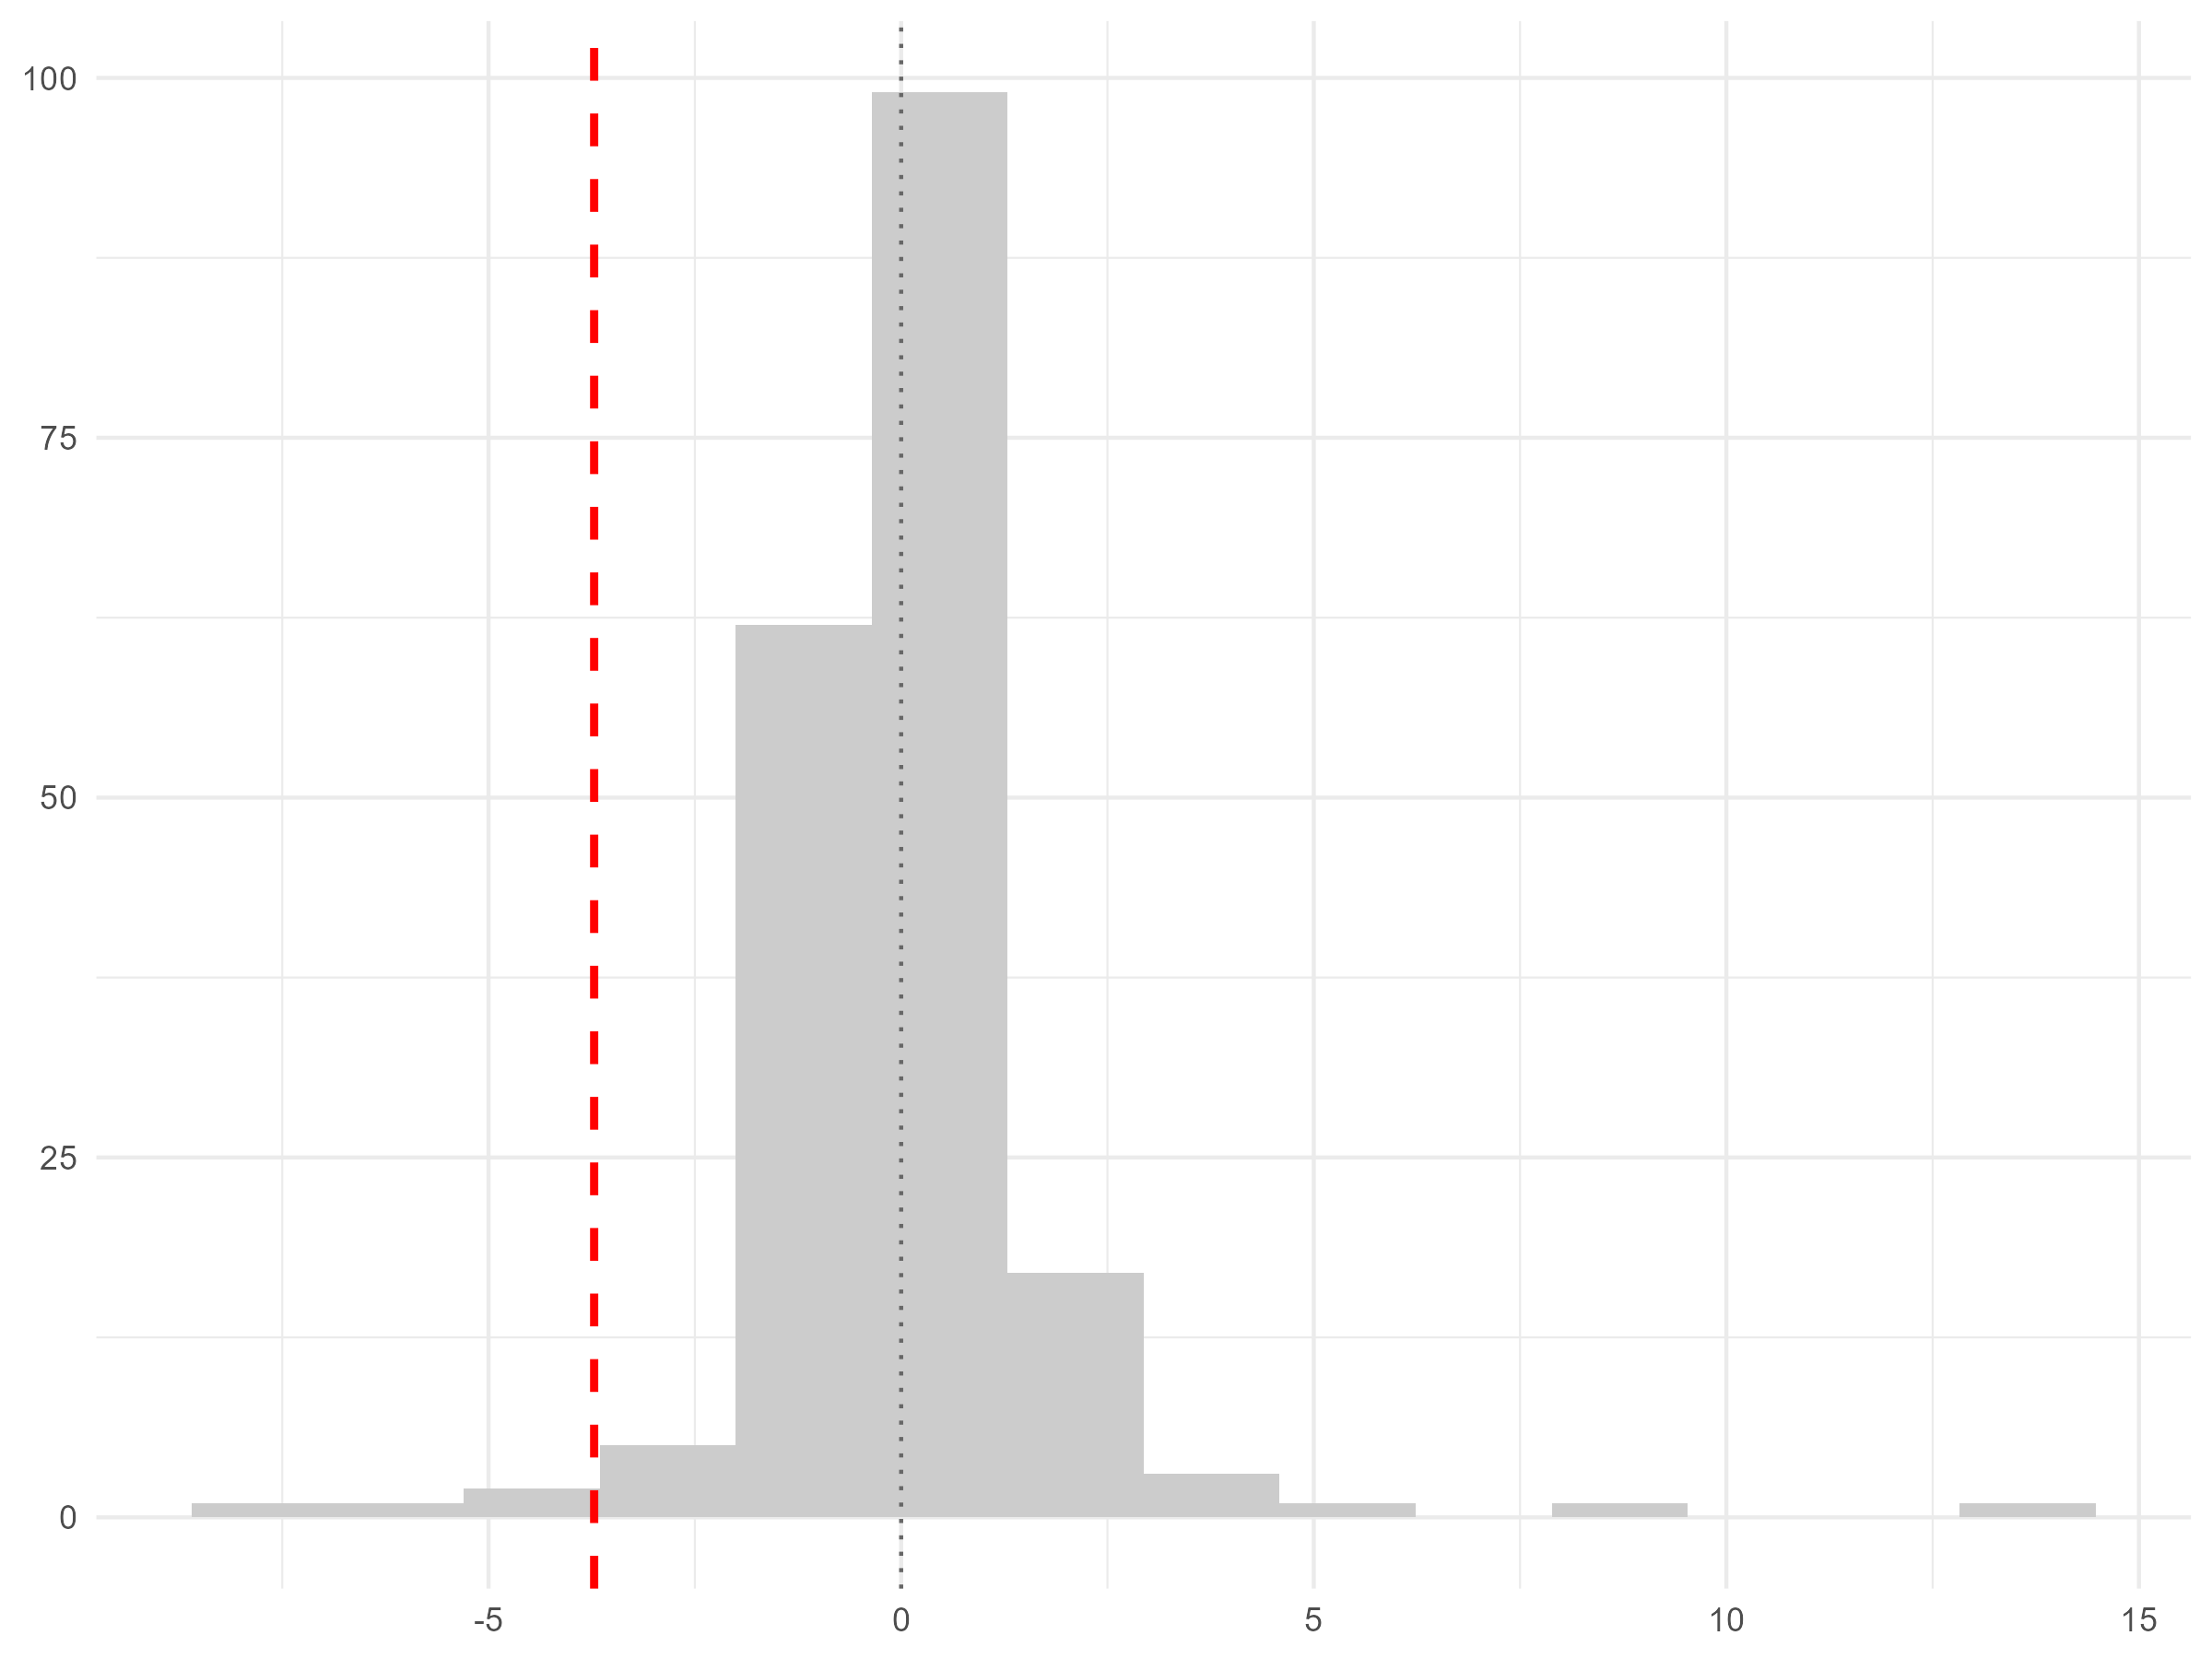
\includegraphics[width=\textwidth]{municipio_4306767_completo_permutacao_direta.png}
\end{minipage}\hfill
\begin{minipage}{0.48\textwidth}
\centering
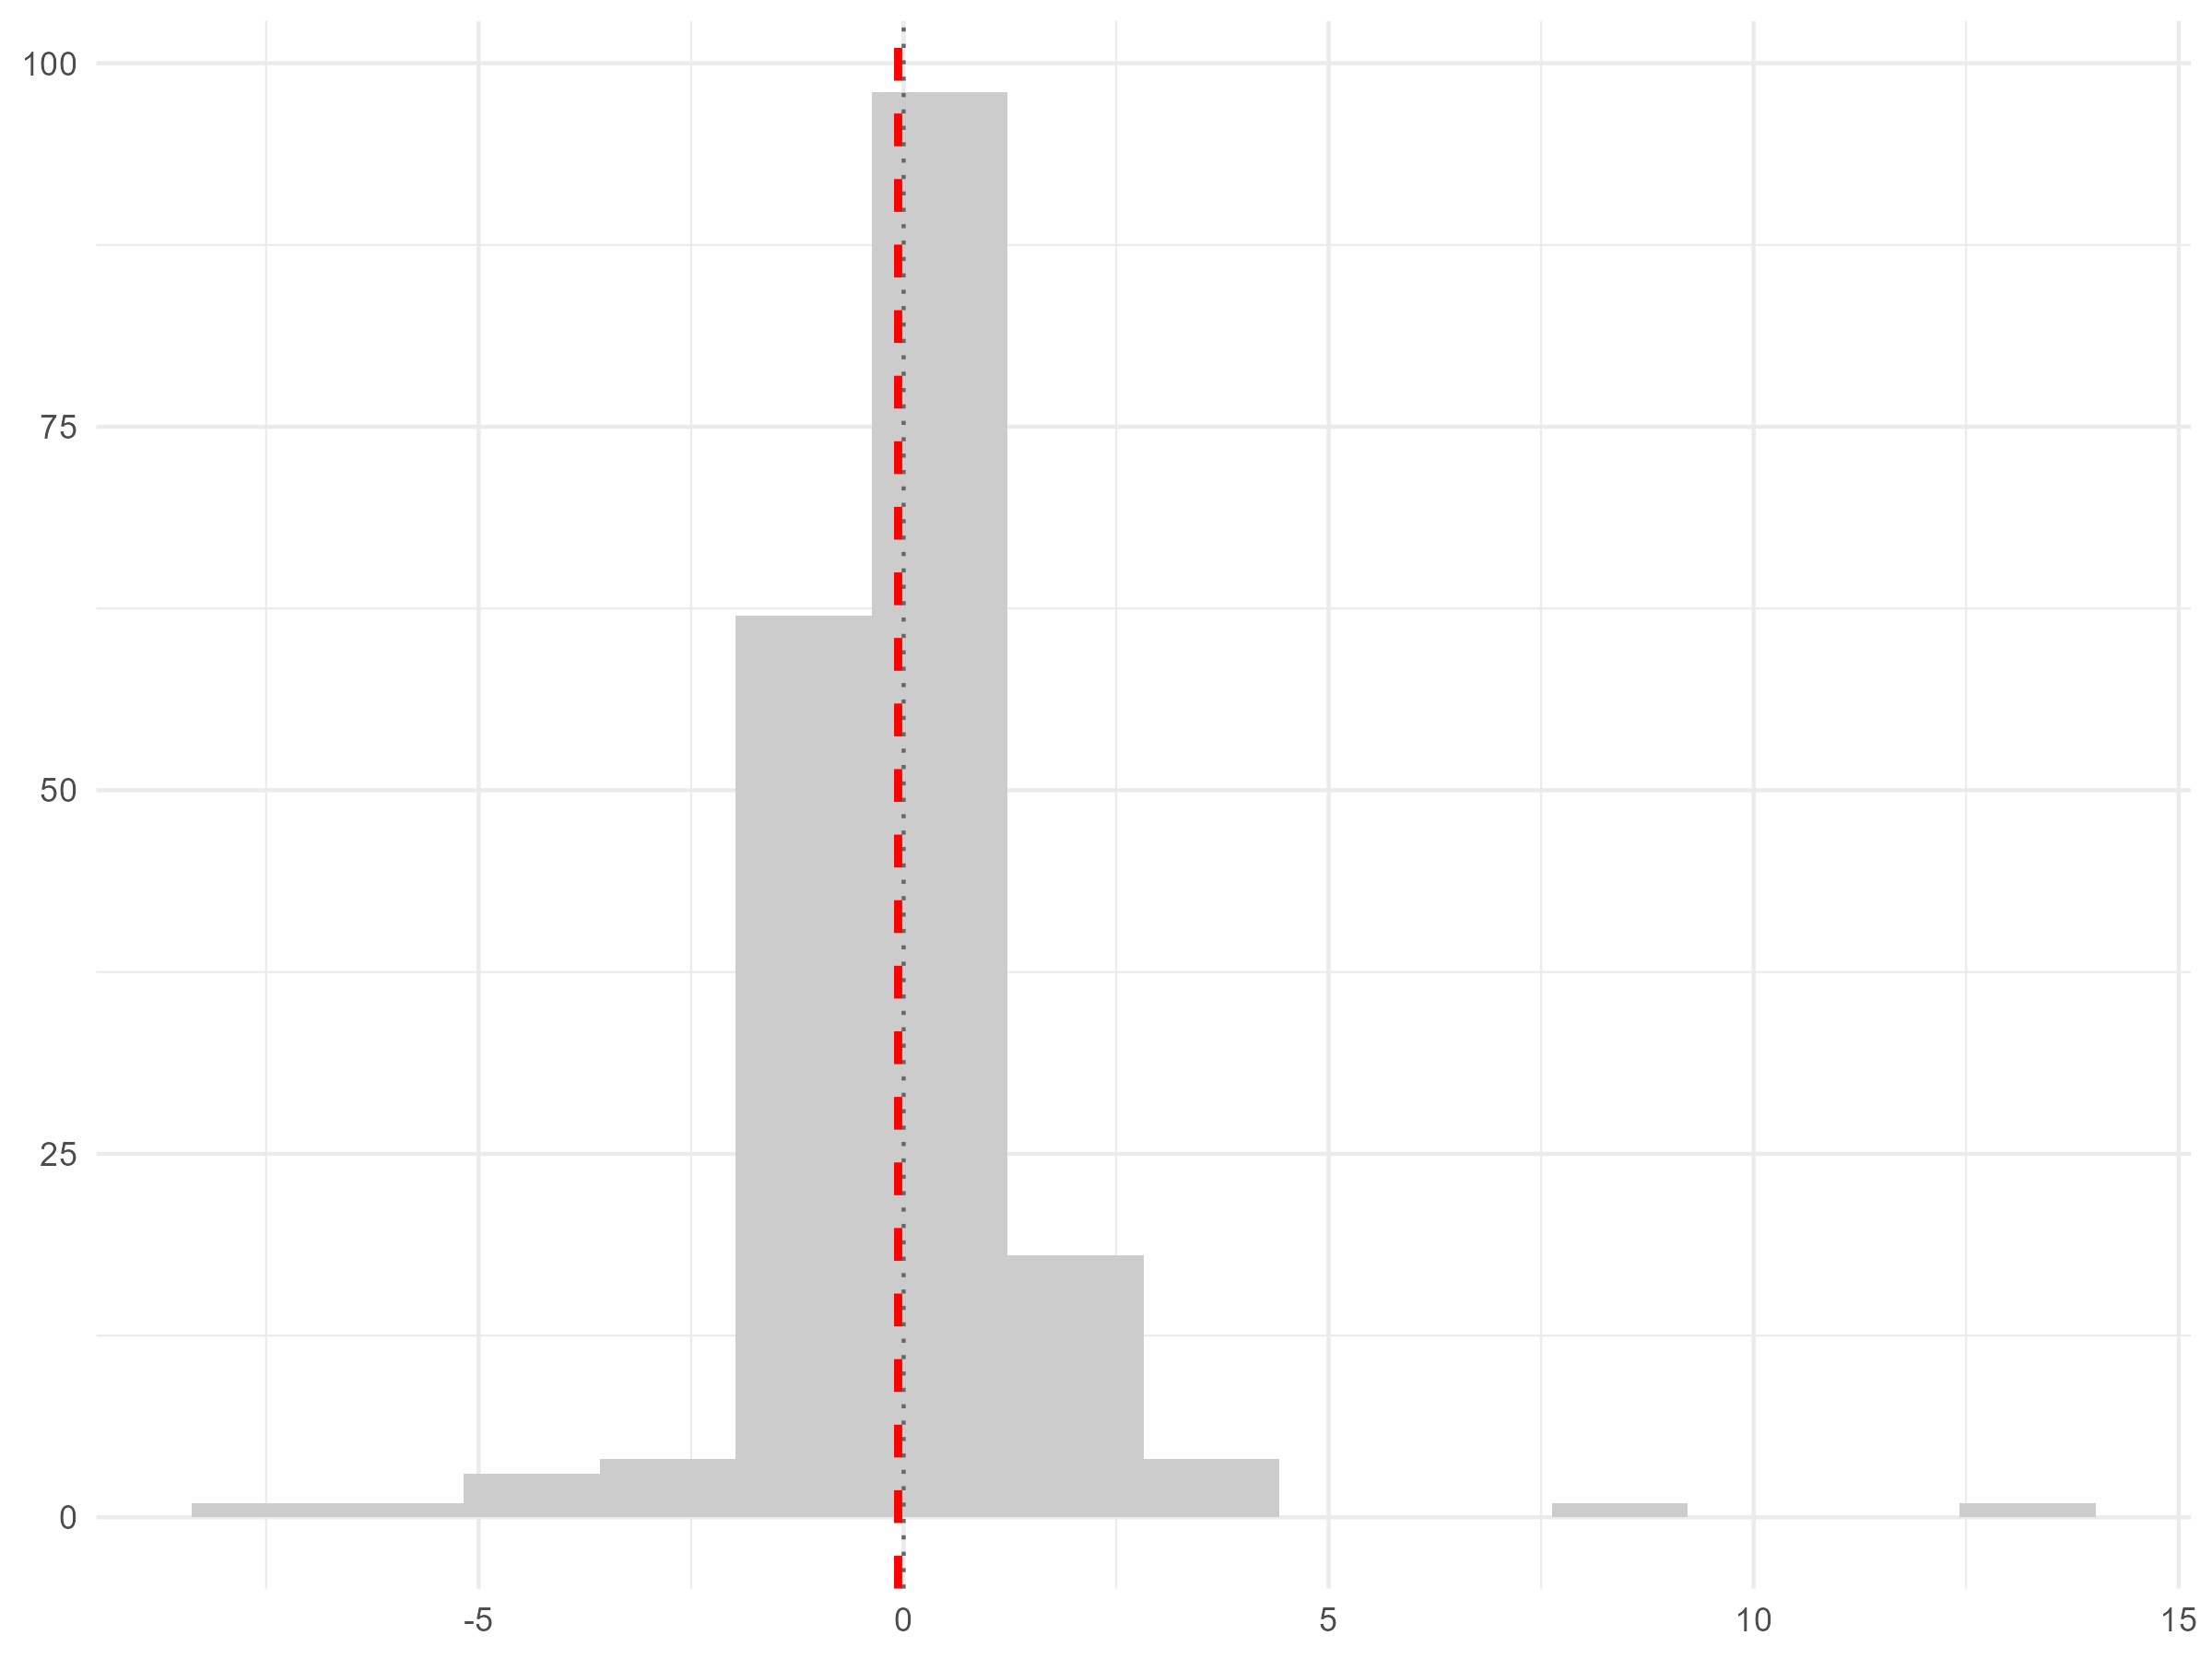
\includegraphics[width=\textwidth]{municipio_4300851_completo_permutacao_direta.png}
\end{minipage}
\caption{Distribuição de efeitos placebo (permutação direta no espaço). À
esquerda, Eldorado do Sul (efeito real na cauda inferior; $p_{bi}=0{,}041$); à
direita, Arambaré (efeito real no centro da distribuição; $p_{bi}=0{,}943$). A
linha vermelha tracejada marca o efeito estimado para a unidade tratada.
Fonte: elaboração própria.}
\label{fig:permutacao}
\end{figure}

A robustez das estimativas à composição do pool doador foi avaliada reestimando o SDiD
para os quatro municípios com efeito robusto ou provável (Eldorado do Sul, Mu\c{c}um,
Roca Sales e Travesseiro) sob quatro limiares alternativos de exclusão: $0{,}5\%$
(baseline), $1\%$, $5\%$ e $10\%$ da população atingida, expandindo o pool de
$N_0 = 193$ a $N_0 = 291$ doadores.

\begin{table}[htbp]
\centering
\caption{Sensibilidade do ATT ao limiar de exclusão do pool doador (SDiD, modo completo)}
\label{tab:sensibilidade}
\begin{threeparttable}
\small
\begin{tabular}{l c c c c}
\toprule
Município & $0{,}5\%$ ($N_0\!=\!193$) & $1\%$ ($N_0\!=\!216$) & $5\%$ ($N_0\!=\!263$) & $10\%$ ($N_0\!=\!291$) \\
\midrule
Eldorado do Sul & $-3{,}72^{*}$ & $-3{,}76^{*}$ & $-3{,}61^{*}$ & $-3{,}68^{*}$ \\
Mu\c{c}um       & $-5{,}08^{*}$ & $-5{,}16^{*}$ & $-5{,}40^{*}$ & $-5{,}25^{*}$ \\
Roca Sales      & $-3{,}72^{*}$ & $-3{,}69^{*}$ & $-3{,}38^{*}$ & $-3{,}33^{*}$ \\
Travesseiro     & $-3{,}73^{*}$ & $-3{,}49^{*}$ & $-3{,}32^{*}$ & $-3{,}15^{*}$ \\
\bottomrule
\end{tabular}
\begin{tablenotes}[flushleft]
\footnotesize
\item ATT em admissões por mil hab./mês. $^{*}$ IC95\% por permutação direta exclui zero
($p < 0{,}05$ em todos os 16 casos). ICs completos na Figura~\ref{fig:sensibilidade}.
\item Amplitude máxima entre limiares: $0{,}6$ adm./mil hab.\ ($< 15\%$ da estimativa baseline).
\item Fonte: elaboração própria a partir de microdados do CAGED.
\end{tablenotes}
\end{threeparttable}
\end{table}

Os resultados revelam estabilidade notável: todos os dezesseis ATTs são negativos e
estatisticamente significantes a $5\%$, com variação máxima entre limiares inferior a
$0{,}6$ admissão por mil habitante, menos de $15\%$ da estimativa baseline,
afastando a hipótese de contaminação do contrafactual por municípios parcialmente
afetados (Seção~\ref{sub:pool}).

\begin{figure}[htbp]
\centering
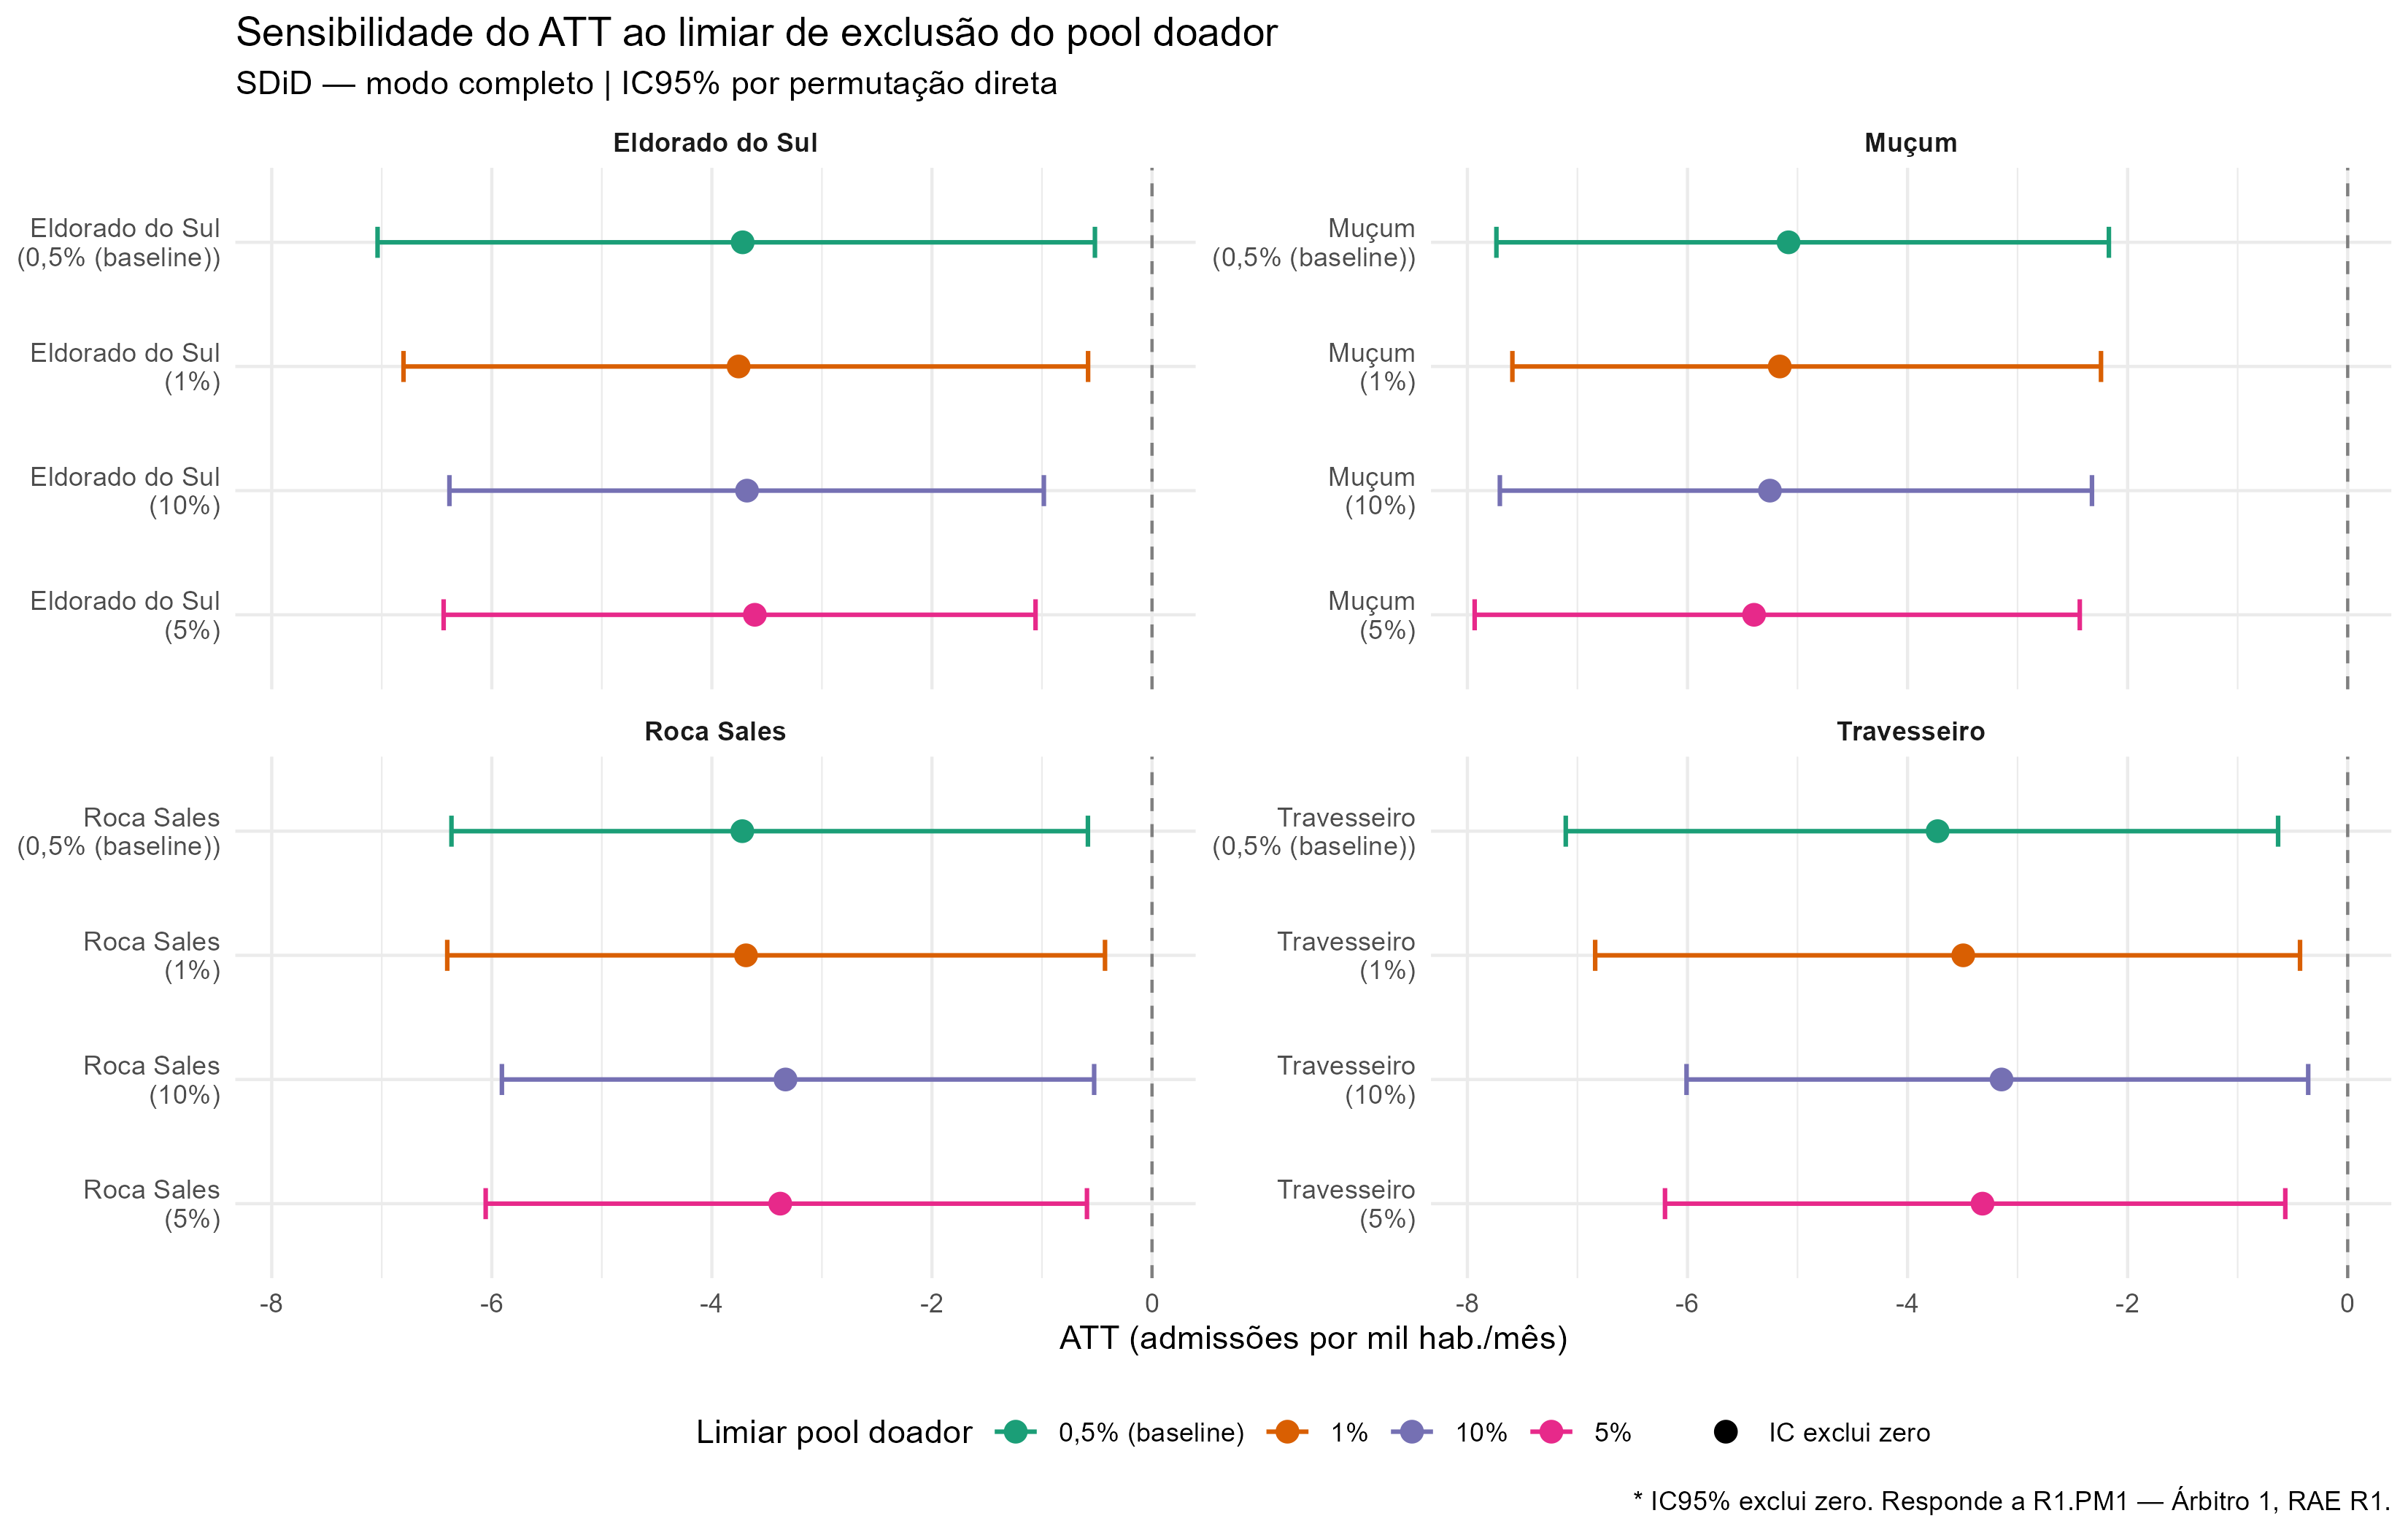
\includegraphics[width=0.95\textwidth]{sensibilidade_forest.png}
\caption{Sensibilidade do ATT ao limiar de exclusão do pool doador (SDiD, modo
completo). Cada cor representa um limiar alternativo ($N_0$ entre 193 e 291 doadores).
Círculos cheios: IC95\% exclui zero; vazios: inclui zero. IC95\% por permutação direta.
Fonte: elaboração própria.}
\label{fig:sensibilidade}
\end{figure}

\newpage
% =====================================================================
\subsection{Triangulação metodológica: TWFE-DiD, SC e SDiD}
\label{sub:triangulacao}

A robustez das estimativas frente à escolha do estimador é avaliada
estimando-se o ATT de cada município pelos três métodos descritos na
Seção~\ref{sec:metodologia} (TWFE-DiD, Controle Sintético e SDiD) sobre
exatamente o mesmo painel, mesma janela e mesmo pool de doadores. Trata-se,
ao nosso conhecimento, da primeira aplicação de uma triangulação dessa
natureza ao caso brasileiro das enchentes de 2024 e responde à recomendação
da literatura recente de não basear o diagnóstico de desastres em um único
estimador, dada a sensibilidade dos resultados às respectivas premissas de
identificação \cite{botzen2019, cavallo2013}. A
Tabela~\ref{tab:triangulacao} reporta os três pontos com seus intervalos de
$95\%$.

\begin{table}[htbp]
\centering
\caption{Triangulação de estimadores: ATT em admissões por mil habitantes (pool completo, $N_0 = 193$)}
\label{tab:triangulacao}
\begin{threeparttable}
\small
\begin{tabular}{l r r r r}
\toprule
Município & TWFE-DiD\tnote{a} & SC\tnote{b} & SDiD\tnote{b} & Amplitude \\
\midrule
Eldorado do Sul & $-3{,}06$ $[-6{,}76;\,0{,}65]$ & $-3{,}80$ $[-6{,}25;\,0{,}81]$ & $\boldsymbol{-3{,}72}$ $[-7{,}04;\,-0{,}52]$ & 0,74 \\
Mu\c{c}um        & $-4{,}72$ $[-8{,}33;\,-1{,}11]$ & $-2{,}92$ $[-5{,}40;\,1{,}69]$ & $\boldsymbol{-5{,}08}$ $[-7{,}74;\,-2{,}17]$ & 2,16 \\
Roca Sales      & $-3{,}12$ $[-6{,}88;\,0{,}64]$ & $-4{,}12$ $[-6{,}59;\,0{,}50]$ & $\boldsymbol{-3{,}72}$ $[-6{,}37;\,-0{,}58]$ & 1,00 \\
Travesseiro     & $-3{,}65$ $[-7{,}62;\,0{,}32]$ & $-3{,}58$ $[-6{,}05;\,1{,}04]$ & $\boldsymbol{-3{,}73}$ $[-7{,}11;\,-0{,}63]$ & 0,15 \\
Igrejinha       & $-1{,}13$ $[-4{,}61;\,2{,}35]$ & $-0{,}29$ $[-2{,}77;\,4{,}32]$ & $\boldsymbol{-1{,}34}$ $[-4{,}40;\,1{,}78]$ & 1,05 \\
Arambaré        & $-0{,}19$ $[-3{,}89;\,3{,}52]$ & $+0{,}29$ $[-2{,}18;\,4{,}91]$ & $\boldsymbol{-0{,}06}$ $[-3{,}10;\,3{,}03]$ & 0,48 \\
\bottomrule
\end{tabular}
\begin{tablenotes}[flushleft]
\footnotesize
\item[a] TWFE-DiD com erro-padrão clusterizado (\textit{cluster} no município, $G = 199$) e IC95\% gaussiano \cite{bertrand2004}; reportado para comparabilidade com a literatura prévia.
\item[b] SC e SDiD com inferência por permutação direta (IC95\% por quantis empíricos recentrados). Em negrito, a estimativa principal (SDiD).
\item Amplitude $=$ $\max_k \hat{\tau}_k - \min_k \hat{\tau}_k$, $k \in \{\text{DiD, SC, SDiD}\}$, em admissões por mil.
\item Fonte: elaboração própria a partir de microdados do CAGED.
\end{tablenotes}
\end{threeparttable}
\end{table}

Três padrões emergem da comparação. Primeiro, todos os municípios com
``efeito robusto'' apresentam \emph{convergência de sinal} entre os três
estimadores e \emph{amplitudes contidas}. Travesseiro é o caso mais ilustrativo,
com amplitude de apenas $0{,}15$ admissões por mil entre TWFE-DiD ($-3{,}65$),
SC ($-3{,}58$) e SDiD ($-3{,}73$); Eldorado do Sul exibe amplitude de $0{,}74$
e Roca Sales de $1{,}00$. Tal convergência fornece um tipo de evidência que
nenhum estimador isolado oferece: o sinal e a ordem de grandeza do choque
são invariantes ao conjunto de premissas de identificação assumidas, o que
constitui o critério prático de robustez por triangulação metodológica
\cite{abadie2021, chaisemartin2020}. Cabe notar que o TWFE-DiD é incluído
sobretudo para comparabilidade com a literatura prévia \cite{teixeira2024}
e deve ser lido com cautela adicional, dado que o teste $F$ conjunto rejeita
a hipótese de tendências paralelas ($F=4{,}14$; $p<0{,}001$). Precisamente
por isso, a convergência de magnitude entre TWFE-DiD e SDiD é
\emph{mais informativa do que parece}: indica que o viés introduzido pela
violação de pré-tendências não é suficientemente grande para alterar a
ordem de grandeza do efeito estimado, reforçando a confiança nas
estimativas do SDiD como estratégia principal.

Segundo, em todos os casos de efeito robusto o SDiD situa-se \emph{entre} o
TWFE-DiD e o SC. Esse comportamento é teoricamente esperado:
\citeonline{arkhangelsky2021} demonstram que o SDiD se aproxima do TWFE
quando as tendências pré-tratamento são paralelas (caso em que os pesos
temporais $\hat{\lambda}_t$ se aproximam de $1/T_0$) e do SC quando há
divergência sistemática nas trajetórias pré-evento. A posição intermediária
observada empiricamente é consistente com um cenário em que as tendências
pré-tratamento dos municípios atingidos divergem moderadamente do pool, o que
o SDiD reequilibra via $\hat{w}_i$ e $\hat{\lambda}_t$ simultaneamente.

Terceiro, em Mu\c{c}um a amplitude entre estimadores é a mais alta ($2{,}16$),
e o SC produz a estimativa de menor magnitude ($-2{,}92$) e único IC95\% que
cruza o zero. Esse comportamento é coerente com a limitação do SC em
contextos de RMSPE pré elevado: quando o pool doador não permite
reproduzir adequadamente a trajetória pré-tratamento da unidade tratada,
parte do efeito real é absorvida pelo viés de ajuste, atenuando a estimativa
\cite{abadie2010, abadie2021}. O SDiD, ao incorporar pesos temporais ótimos,
acomoda parcialmente a má aderência pré-tratamento, gerando estimativa mais
próxima daquela do TWFE-DiD \cite{arkhangelsky2021}.
Esse caso ilustra com clareza por que a
escolha de um estimador isolado para diagnósticos de desastre pode produzir
conclusões divergentes a partir do mesmo dado, e por que a recomendação de
\citeonline{botzen2019} de reportar múltiplos estimadores deve ser tratada
como prática mínima na literatura de avaliação de desastres climáticos, quando os dados permitirem.

Em Arambaré e Igrejinha, todos os três estimadores produzem intervalos que
cruzam o zero, e em Arambaré o sinal é discordante entre SC ($+0{,}29$) e os
demais ($-0{,}19$ e $-0{,}06$). A divergência de sinal nesse caso, longe de
um problema, é informativa: indica que nenhum dos três estimadores consegue
afastar a hipótese nula de ausência de efeito, e a discordância de sinal é
ruído estatístico em torno de zero, exatamente o padrão esperado quando
não há tratamento detectável.

Cabe um esclarecimento importante: a ``convergência'' aqui discutida refere-se à
concordância de \emph{sinal} e de \emph{ordem de grandeza} das estimativas
pontuais, e não à significância estatística. Para a maioria dos municípios, os ICs
do TWFE-DiD e do SC cruzam zero, enquanto apenas o SDiD alcança significância
convencional a $5\%$. Isso reflete, em parte, mecanismos de inferência com
potências distintas: o TWFE-DiD usa ICs gaussianos sem rebalanceamento de
trajetórias; o SC, estimado unidade a unidade sobre 193 doadores, produz quantis
empíricos mais dispersos por não incorporar os pesos de tempo $\hat{\lambda}_t$.
O SDiD combina o rebalanceamento duplo ($\hat{w}_i$ e $\hat{\lambda}_t$) com a
distribuição exata de permutação sobre os 193 placebos, conferindo-lhe maior
potência para detectar sinais consistentes em configurações com poucos tratados,
propriedade documentada em simulações de Monte Carlo por
\citeonline{arkhangelsky2021}. A não-significância do TWFE-DiD e do SC não
contradiz os resultados: ela é em parte estrutural ao procedimento de inferência
de cada estimador e reforça, por contraste, a adequação do SDiD como estratégia
principal neste contexto.

A Figura~\ref{fig:forest} apresenta o
\textit{forest plot} da triangulação, facetado por município.

\begin{figure}[htbp]
\centering
\includegraphics[width=0.95\textwidth]{triangulacao_forest.png}
\caption{Triangulação de estimadores: TWFE-DiD, Controle Sintético (SC) e SDiD
(pool completo, $N_0 = 193$). Pontos representam a estimativa pontual do ATT;
barras horizontais, o IC95\%. \textbf{Cor:} vermelho = IC95\% exclui zero;
cinza = IC95\% cruza zero. \textbf{Forma/traço:} círculo com linha contínua
($\bullet$—) = inferência por permutação direta (SC e SDiD); triângulo com
linha tracejada ($\blacktriangle$\,--\,--) = IC gaussiano por EP placebo
(TWFE-DiD). Fonte: elaboração própria.}
\label{fig:forest}
\end{figure}

O estudo de evento TWFE-DiD fornece um diagnóstico complementar da suposição de
tendências paralelas, estimando a especificação dinâmica descrita na
Seção~\ref{sec:metodologia}:
$Y_{it} = \alpha_i + \gamma_t + \sum_{k \neq -1} \delta_k \cdot
\mathbf{1}\{r_{it} = k\} \cdot D_i + \varepsilon_{it}$,
com $r_{it} = t - t^*$, janela $k \in [-12,\,+11]$ e referência $k = -1$
(abril/2024). A Figura~\ref{fig:event_study} apresenta os coeficientes estimados
com IC95\% \textit{cluster-robust} no município.

\begin{figure}[htbp]
\centering
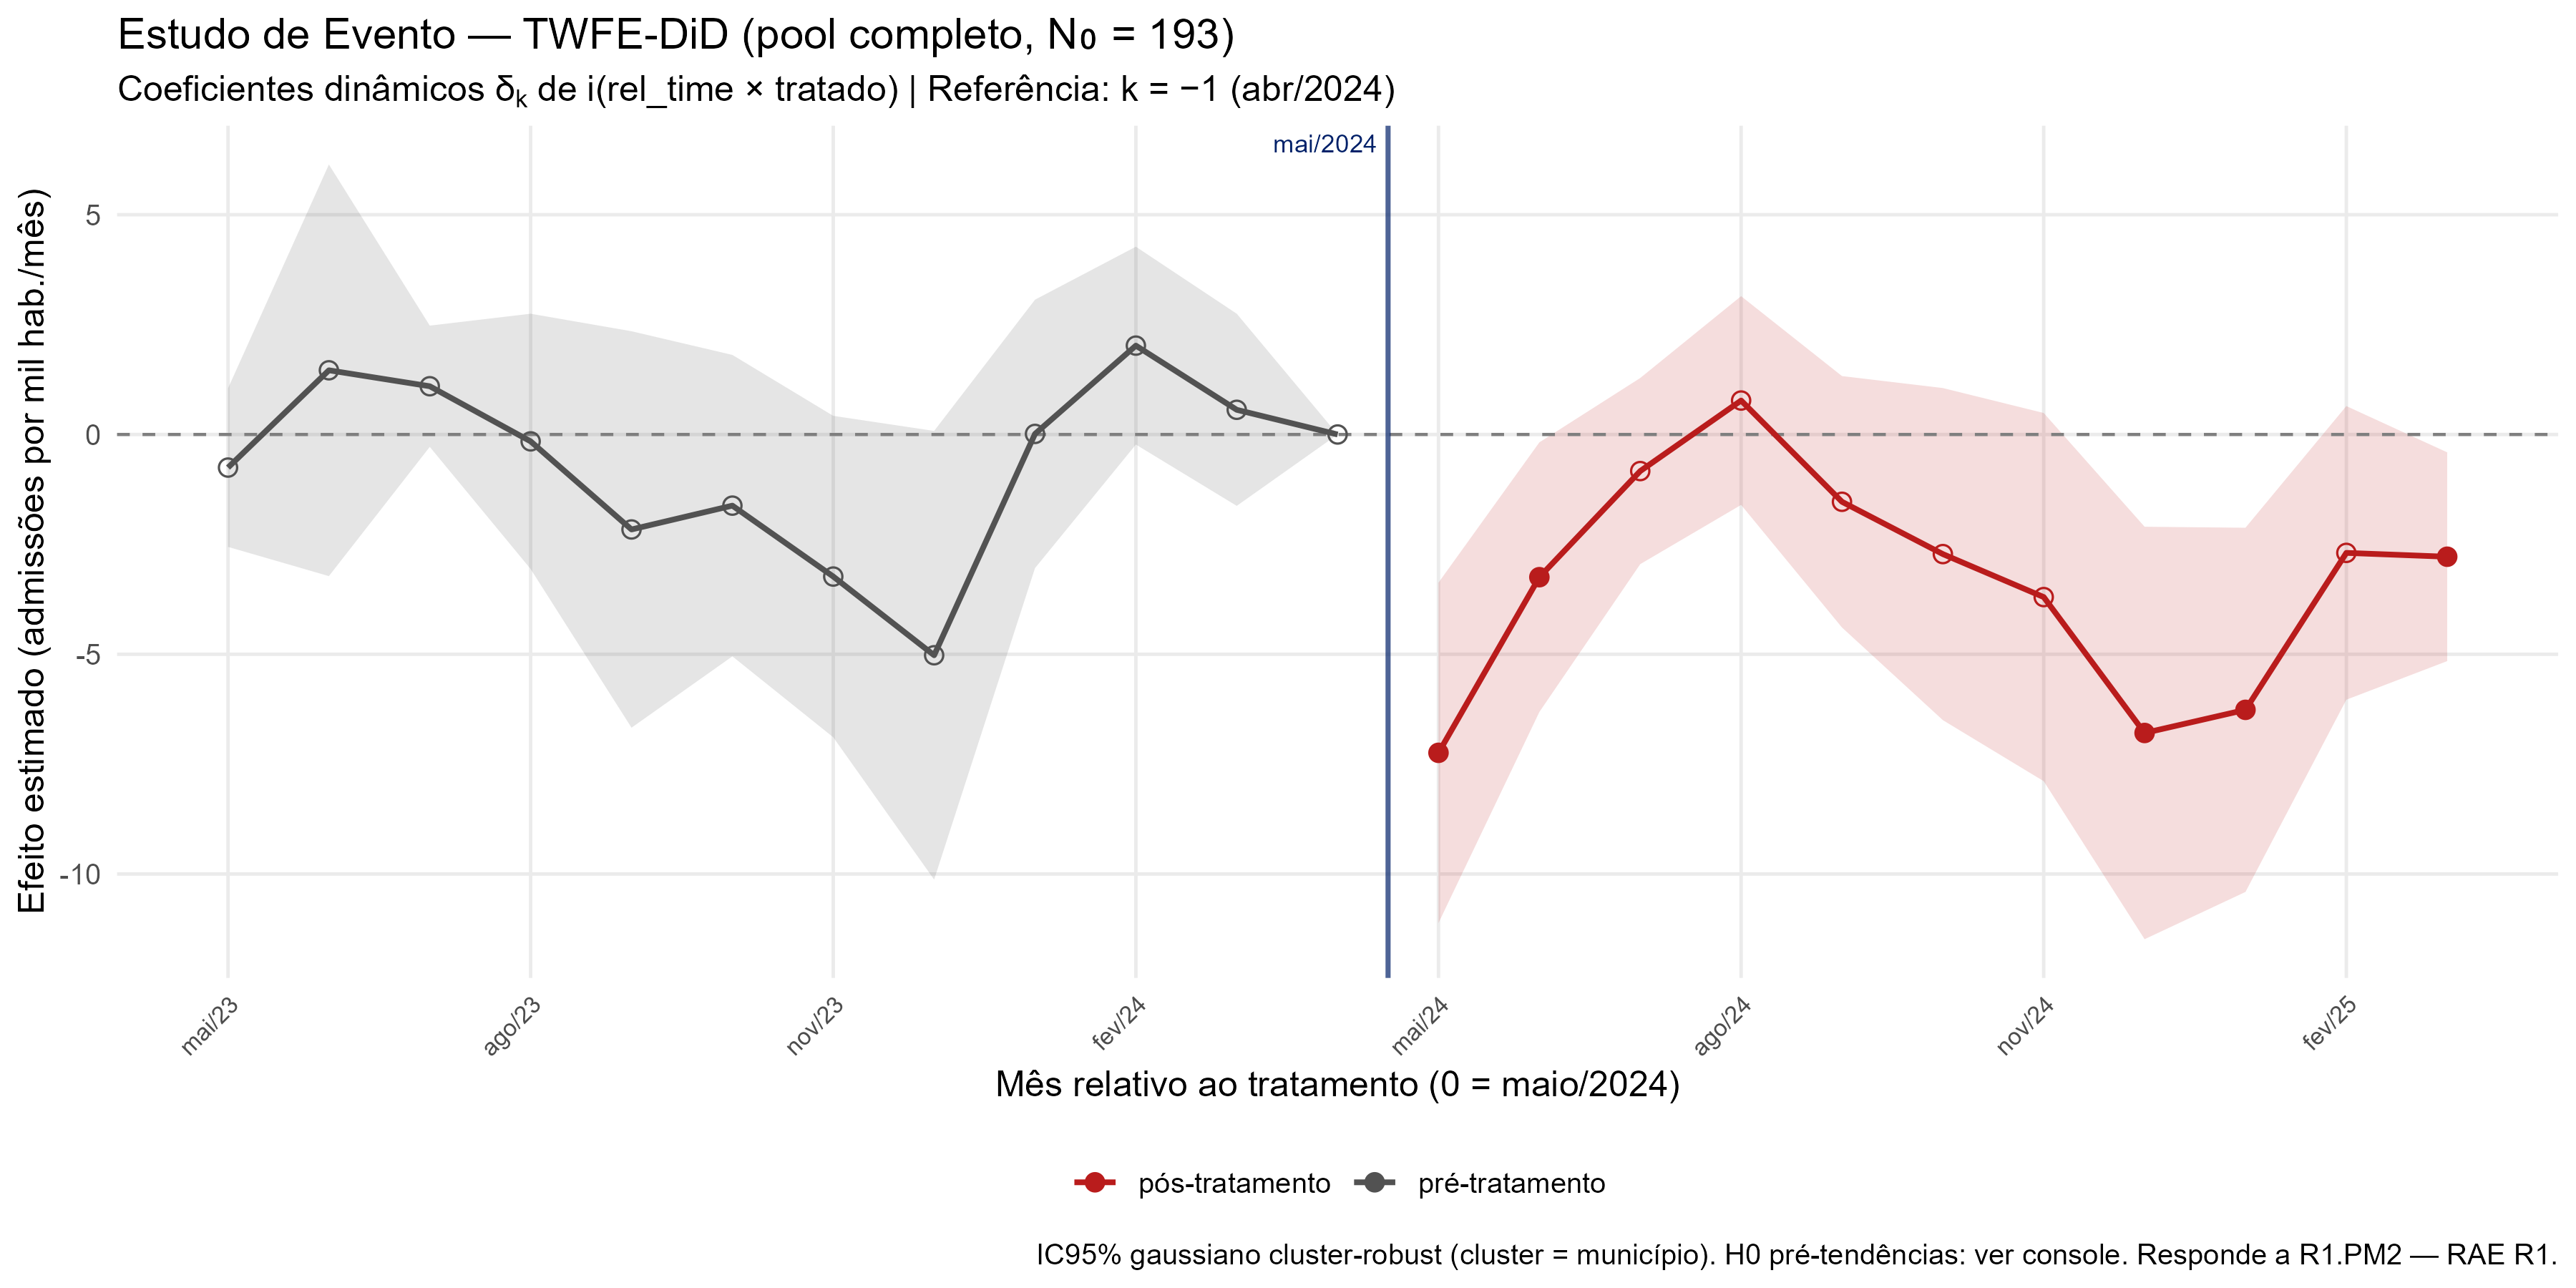
\includegraphics[width=0.95\textwidth]{event_study_twfe_todos.png}
\caption{Estudo de evento TWFE-DiD: coeficientes dinâmicos $\hat{\delta}_k$ com
IC95\% \textit{cluster-robust}. Linha vertical: $k = 0$ (mai./2024); referência
$\hat{\delta}_{-1} = 0$ por normalização. Círculos cheios: IC95\% exclui zero.
$N = 199$ municípios, $T = 51$ períodos. Fonte: elaboração própria.}
\label{fig:event_study}
\end{figure}

Individualmente, nenhum dos onze coeficientes pré-tratamento é significante a $5\%$.
O teste $F$ conjunto, contudo, rejeita a nulidade conjunta
($F = 4{,}14$; $p < 0{,}001$; $g.l. = 11;\,198$), indicando que as trajetórias dos
municípios tratados divergem sistematicamente das unidades de controle no TWFE sem
\textit{reweighting}. Esse diagnóstico confirma, \textit{ex post}, a adequação do SDiD
como estimador principal: seus pesos $\hat{w}_i$ e $\hat{\lambda}_t$ reequilibram
exatamente as trajetórias que o TWFE canônico não consegue harmonizar
\cite{arkhangelsky2021}. A seleção geográfica das áreas de risco produz precisamente esse
padrão de pré-tendências divergentes, coerente com o argumento de
\citeonline{elsner2024} sobre a necessidade de estratégias de estimação que acomodem
essa heterogeneidade estrutural. No período pós-evento, o coeficiente de impacto
imediato $\hat{\delta}_0 = -7{,}24$ ($p < 0{,}001$) reproduz o choque de maio/2024,
e os picos em $\hat{\delta}_7$ e $\hat{\delta}_8$ ($-6{,}79$ e $-6{,}27$,
ambos $p < 0{,}01$) são consistentes com a segunda onda de retração identificada
na Subseção~\ref{sub:acumulado}.

\newpage

% =====================================================================
\subsection{Trajetórias mensais e efeito acumulado em postos de trabalho}
\label{sub:acumulado}

A reportagem do ATT médio oculta a dinâmica temporal do choque, central para
a discussão de política pública. A Figura~\ref{fig:acumulado_es} apresenta o
efeito acumulado em Eldorado do Sul ao longo dos onze meses pós-desastre,
com banda de IC$95\%$ obtida por placebo na curva.

\begin{figure}[htbp]
\centering
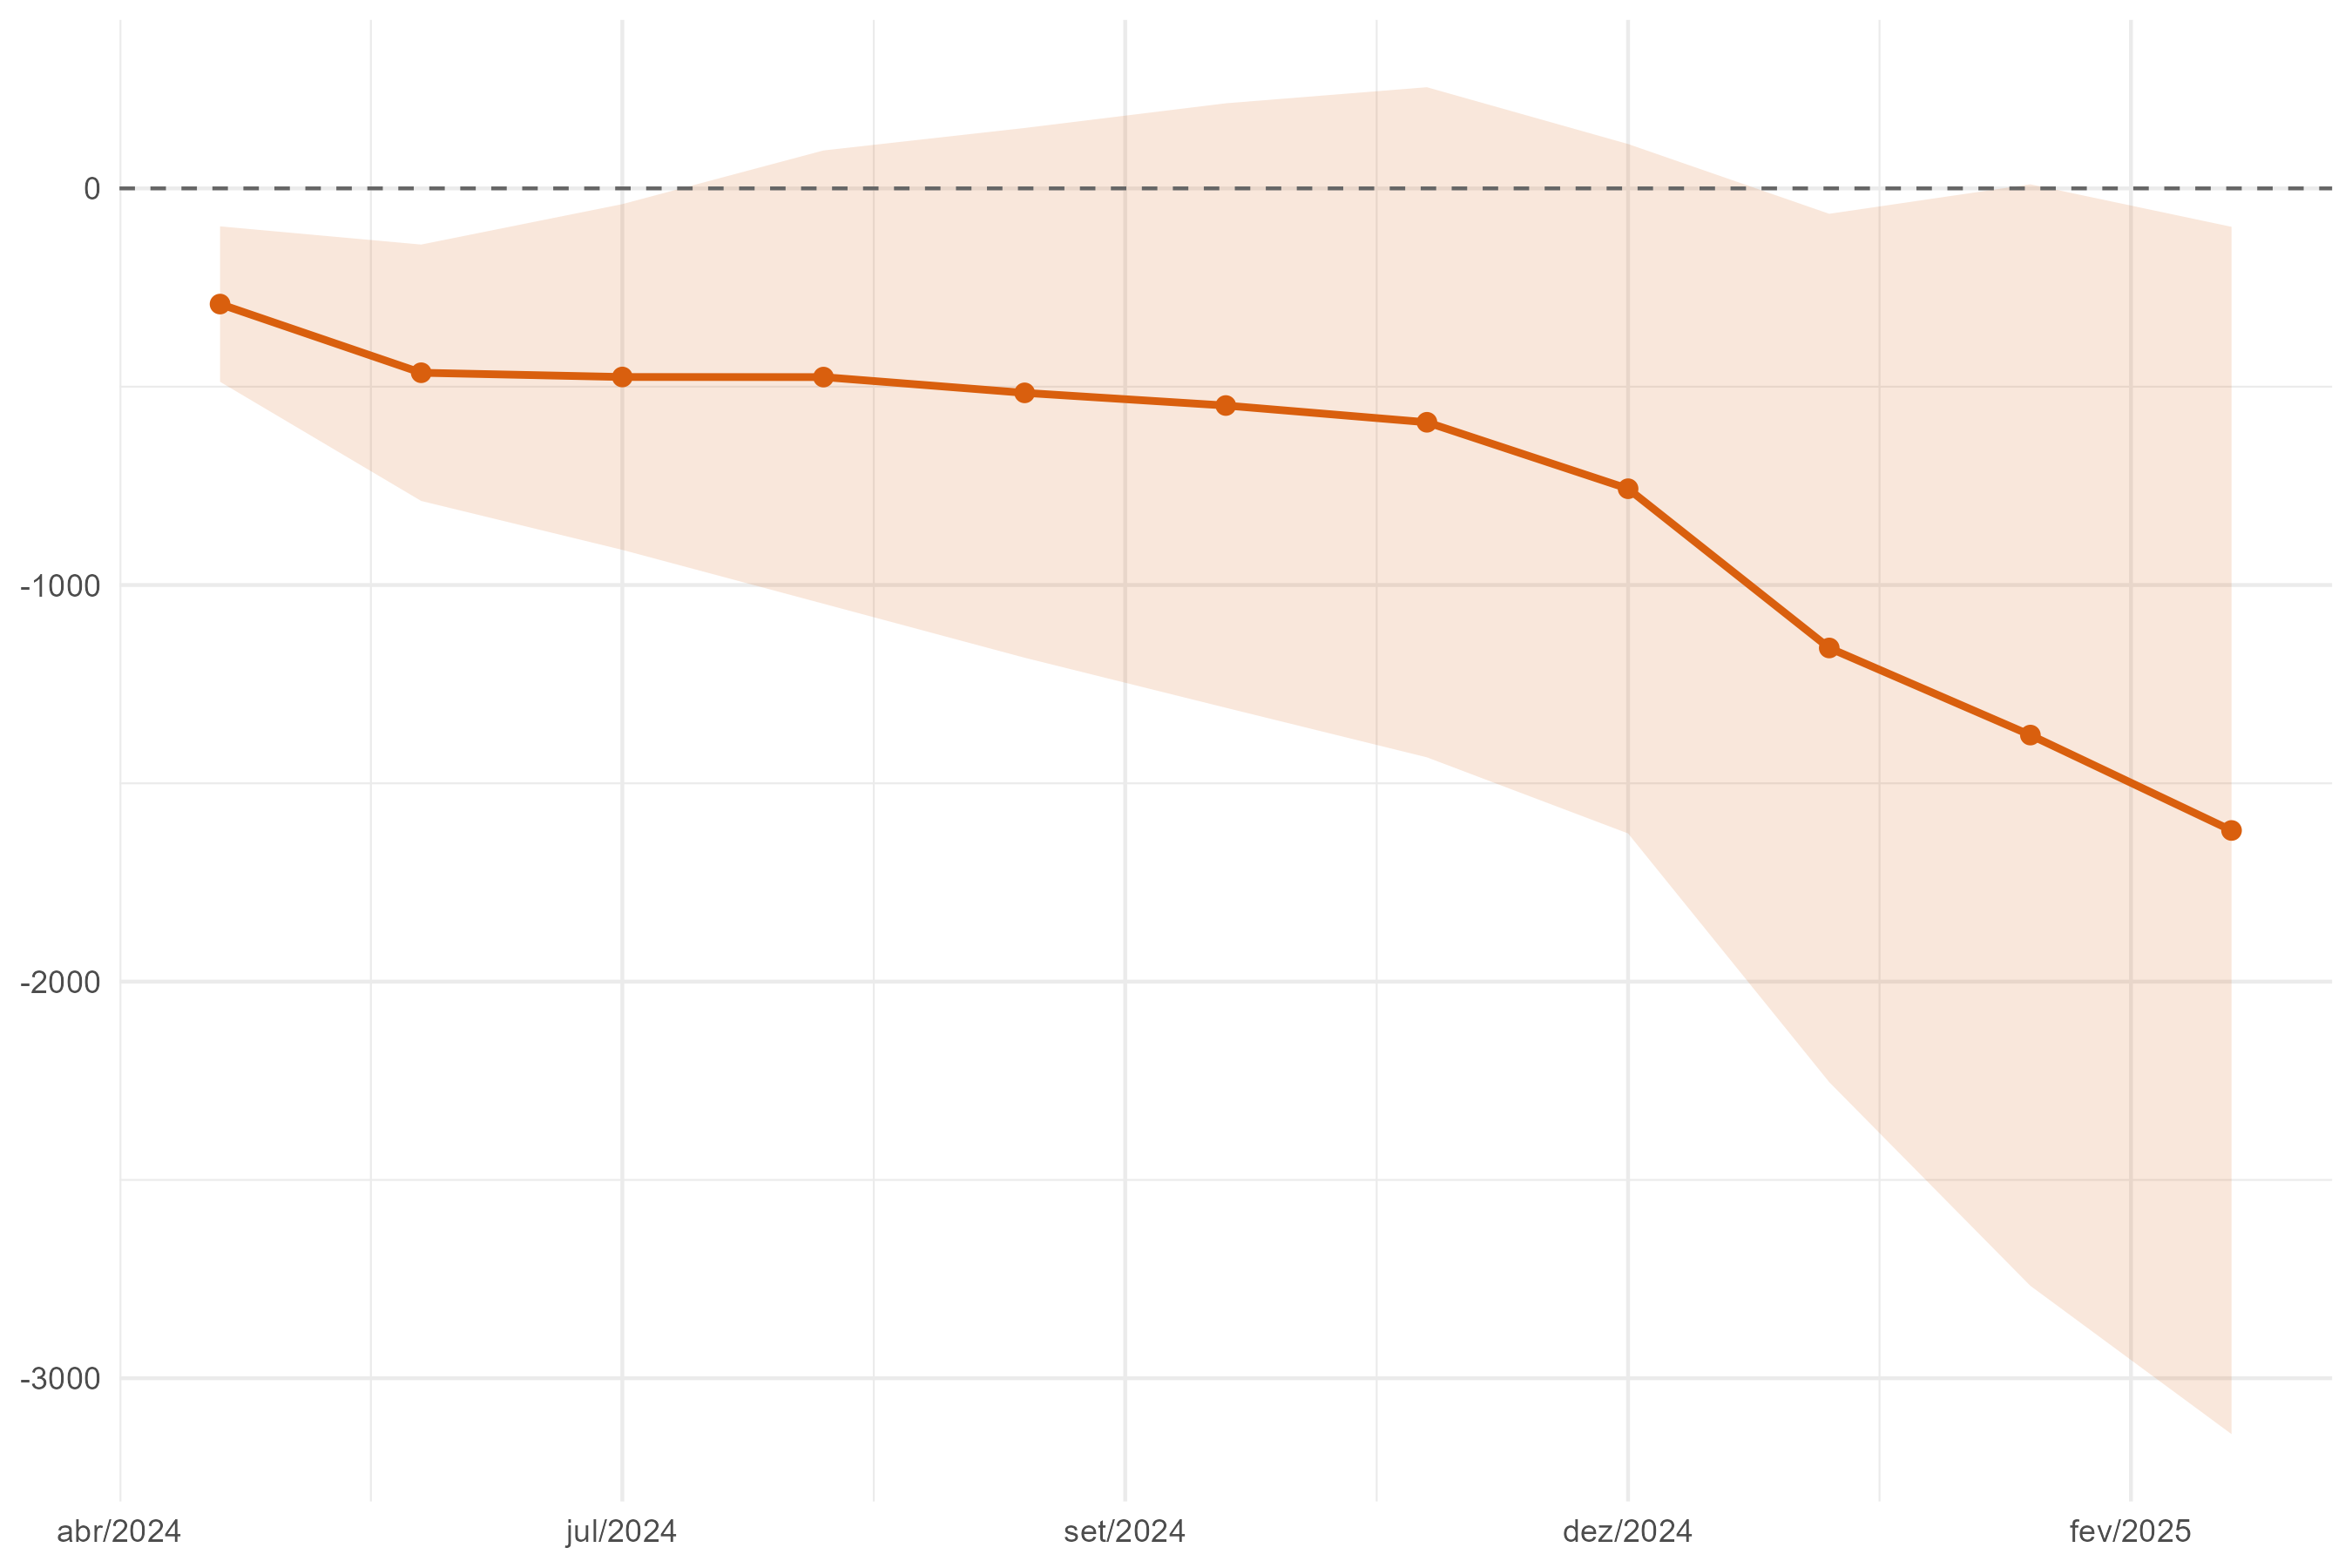
\includegraphics[width=0.85\textwidth]{municipio_4306767_completo_efeito_acumulado.png}
\caption{Efeito acumulado sobre admissões formais: Eldorado do Sul. Banda
laranja: IC95\% por placebo na curva sobre os doadores. Fonte: elaboração
própria.}
\label{fig:acumulado_es}
\end{figure}
\newpage
A dinâmica mensal revela um padrão coerente com o relato físico do desastre.
Em Eldorado do Sul, o choque inicial em maio de 2024 (efeito de $-7{,}37$
admissões por mil) é consistente com a interrupção da atividade econômica
durante o período de inundação; segue-se uma fase intermediária com
efeitos de menor magnitude entre junho e novembro, sugestiva de uma retomada
parcial da produção sob possíveis restrições logísticas; e há um segundo
pico de retração no início de 2025: janeiro registra o maior efeito negativo
da série, $-10{,}15$ por mil. Como o pool pré-tratamento incorpora quatro
Januários anteriores ao choque (2021--2024), o controle sintético replica o
padrão sazonal histórico de janeiro; o efeito de $-10{,}15$ é, portanto,
estimado \emph{relativo} ao nível sazonal esperado, e não à sazonalidade
bruta do mês. Esse padrão em ``W'' é consistente com a hipótese de
\citeonline{xiao2014} de que danos à infraestrutura de transporte geram
efeitos persistentes sobre os custos de operação, postergando a recuperação
plena do mercado de trabalho local. As estimativas por mil
habitantes traduzem-se em perdas absolutas de admissões formais quando
reescaladas pela população municipal e somadas mês a mês. A
Tabela~\ref{tab:acumulado} reporta o efeito acumulado em postos de trabalho.

\begin{table}[htbp]
\centering
\caption{Efeito acumulado sobre admissões formais (onze meses pós-desastre, mai./2024–mar./2025)}
\label{tab:acumulado}
\begin{threeparttable}
\small
\begin{tabular}{l r r r}
\toprule
Município & Pop. (2022) & Efeito acum. (admissões) & IC95\% (perm.) \\
\midrule
Eldorado do Sul & 39.559 & $-1.619$ & $[-3.141;\,-97]$ \\
Mu\c{c}um        & 4.601  & $-257$   & $[-434;\,-80]$ \\
Roca Sales      & 10.418 & $-427$   & $[-828;\,-26]$ \\
Travesseiro     & 2.152  & $-88$    & $[-171;\,-5]$ \\
Igrejinha       & 32.808 & $-485$   & $[-1.747;\,777]$ \\
Arambaré        & 4.112  & $-3$     & $[-161;\,155]$ \\
\bottomrule
\end{tabular}
\begin{tablenotes}[flushleft]
\footnotesize
\item Efeito acumulado calculado como soma da curva mensal de efeito sobre admissões reescalada pela população (Censo 2022). IC95\% por placebo na curva acumulada.
\item Fonte: elaboração própria a partir de microdados do CAGED e Censo Demográfico 2022 (IBGE).
\end{tablenotes}
\end{threeparttable}
\end{table}

Em termos absolutos, o desastre suprimiu aproximadamente $1.619$ admissões
formais em Eldorado do Sul ao longo dos onze meses analisados (equivalente
a cerca de $4\%$ da população do município), $427$ em Roca Sales, $257$ em
Mu\c{c}um e $88$ em Travesseiro. Para os quatro municípios com efeito robusto
ou provável, o déficit somado supera $2.390$ admissões formais. Esses
números representam estritamente o componente \emph{dinâmico} do mercado de
trabalho, ou seja, as oportunidades de emprego que \emph{não} foram criadas em
razão do choque; não incluem o efeito sobre desligamentos, que
\citeonline{teixeira2024} mostraram ser estatisticamente nulo na agregação
municipal, provavelmente em decorrência da rigidez da legislação trabalhista
brasileira e das políticas de manutenção do emprego vigentes no período.
A interpretação dos absolutos exige, portanto, a leitura conjunta: o ajuste
do emprego formal ao desastre se deu predominantemente pelo bloqueio da
\emph{margem de entrada}, e é essa margem que as estimativas acima
quantificam.


% =====================================================================
\subsection{Heterogeneidade do efeito e canais de dano}
\label{sub:heterogeneidade}

A dissociação entre exposição residencial e resposta do emprego (Arambaré
e Igrejinha apresentam, respectivamente, $51{,}9\%$ e $50{,}9\%$ dos
domicílios atingidos, mas não exibem efeito significante) motiva a
investigação dos canais pelos quais o desastre se transmite ao mercado de
trabalho formal. A literatura de economia de desastres distingue, entre
outros, dois mecanismos centrais: o canal de \emph{capital/firma}
(destruição de estabelecimentos reduz diretamente a demanda por trabalho
\cite{haddad2015economic}) e o canal de \emph{conectividade/logística}
(danos à rede de transporte elevam custos de insumo e de escoamento e interrompem
cadeias produtivas \cite{xiao2014}). Para confrontar esses mecanismos com os
dados, comparam-se variáveis de dano físico (oriundas do Mapa Único do Plano Rio
Grande, MUPRS/SPGG-RS) entre o grupo de municípios ``com efeito''
(os quatro com IC95\% negativo) e o grupo ``sem efeito'' (Igrejinha e
Arambaré).

\begin{quote}
\small\noindent
\textbf{Advertência metodológica.} Esta subseção é \emph{descritiva} e
\emph{geradora de hipóteses}. Com apenas seis unidades ($n=6$), não se conduz
regressão nem inferência formal entre municípios; a leitura é estritamente
associativa, jamais causal no plano intermunicipal. Os auxílios emergenciais
(p.\,ex., Volta por Cima, SOS-RS) foram excluídos do conjunto de covariáveis
de dano por serem pós-tratamento e endógenos ao próprio nível de destruição,
configurando \textit{bad controls} \cite{angrist2009}.
\end{quote}

A Tabela~\ref{tab:het} ordena as variáveis de dano segundo sua capacidade de
\emph{separar} os dois grupos, medida pelo \textit{gap} padronizado ($z$) entre
as médias dos grupos ``com'' e ``sem'' efeito.

\begin{table}[htbp]
\centering
\caption{Ranking de separação entre grupos por variável de dano (descritivo, $n=6$)}
\label{tab:het}
\begin{threeparttable}
\small
\begin{tabular}{l r r r}
\toprule
Variável de dano & \textit{Gap} padronizado ($z$) & Média ``com'' & Média ``sem'' \\
\midrule
Dano viário (\% malha rodoviária)        & 1,49 & 0,373 & 0,275 \\
Dano às famílias (\% famílias)           & 1,39 & 0,763 & 0,583 \\
Dano a firmas (\% CNPJ)                  & 1,37 & 0,756 & 0,528 \\
Índice produtivo relativo\tnote{a}       & 1,00 & 0,113 & 0,004 \\
Dano residencial (\% domicílios)         & 1,00 & 0,643 & 0,525 \\
Equipamentos públicos (\%)               & 0,67 & 0,659 & 0,461 \\
\bottomrule
\end{tabular}
\begin{tablenotes}[flushleft]
\footnotesize
\item[a] Índice produtivo relativo $=$ (\% CNPJ atingidos) $-$ (\% domicílios atingidos): mede a geografia diferencial do dano entre tecido produtivo e residencial.
\item Fonte: elaboração própria a partir do MUPRS/SPGG-RS e dos resultados SDiD.
\end{tablenotes}
\end{threeparttable}
\end{table}

A leitura do ranking é sugestiva e alinhada à teoria. As variáveis que melhor
discriminam os municípios com retração do emprego são o \emph{dano viário}
($z = 1{,}49$) e o \emph{dano a firmas} ($z = 1{,}37$), com o \emph{índice
produtivo relativo} ($z = 1{,}00$) corroborando a importância da geografia
diferencial do dano. O dano \emph{residencial} isolado separa pouco os grupos
($z = 1{,}00$, com médias próximas: $0{,}643$ contra $0{,}525$), coerente com
a observação prévia de que a intensidade do dano às moradias, por si só, não
prediz a resposta do emprego formal. Em outras palavras, são os canais
produtivos (destruição de capital e ruptura de conectividade) que parecem
governar o ajuste do trabalho, em sintonia com o canal de demanda por
trabalho de \citeonline{haddad2015economic} e com a centralidade da infraestrutura
de transporte enfatizada por \citeonline{xiao2014}.

Dois municípios merecem leitura individualizada. Arambaré, sem efeito
detectável, é o único da amostra com índice produtivo relativo
\emph{negativo} ($-0{,}14$): seu tecido produtivo foi proporcionalmente
\emph{poupado} em relação às moradias atingidas, o que é consistente com a
ausência de resposta do emprego formal apesar de mais da metade dos
domicílios afetados. O caso ilustra que a métrica de severidade
convencionalmente utilizada (proporção de população atingida) pode mascarar
a heterogeneidade do impacto sobre o lado produtivo da economia, ponto que
ecoa a crítica de \citeonline{cavallo2013} de que indicadores agregados de
exposição tendem a obscurecer o canal econômico do desastre.

Igrejinha, por sua vez, constitui a exceção informativa: apresenta danos
viário e a firmas comparáveis aos de municípios com efeito robusto, mas não
exibe resposta significante. Uma hipótese plausível (a ser examinada em
pesquisa futura) é a de que sua economia, maior e mais diversificada
(cerca de $33$ mil habitantes, base industrial de calçados e couro com
ligações ao mercado nacional), tenha maior capacidade de absorção do choque
via realocação setorial e busca de fornecedores alternativos, atenuando a
transmissão do dano físico ao emprego formal. Esse mecanismo de resiliência
por diversificação é destacado por \citeonline{xiao2014} na literatura de
recuperação pós-desastre.

As Figuras~\ref{fig:canais} e \ref{fig:perfilz} sintetizam, respectivamente,
os canais centrais de dano por município e o perfil padronizado de dano de
cada unidade.

\begin{figure}[htbp]
\centering
\includegraphics[width=0.95\textwidth]{dano_canais_centrais.png}
\caption{Canais centrais de dano por município: dano viário, dano a firmas
(CNPJ) e índice produtivo relativo. Verde: municípios com efeito (IC95\%
$<0$); cinza: sem efeito. Fonte: elaboração própria a partir do MUPRS/SPGG-RS.}
\label{fig:canais}
\end{figure}

\begin{figure}[htbp]
\centering
\includegraphics[width=0.95\textwidth]{dano_perfil_z.png}
\caption{Perfil de dano padronizado ($z$-\textit{score}) por município. Cada
linha é um município; valores em $z$ entre os tratados. Fonte: elaboração
própria.}
\label{fig:perfilz}
\end{figure}

\newpage
% =====================================================================
\subsection{Síntese dos resultados}
\label{sub:sintese}

Em conjunto, os achados sustentam quatro conclusões: (i) retração significante e
persistente nos municípios com dano produtivo severo, com efeitos convergentes em
torno de $-3{,}7$ admissões por mil hab./mês nos três municípios com resultado robusto;
(ii) triangulação metodológica com convergência de sinal e ordem de grandeza entre
TWFE-DiD, SC e SDiD nos municípios com efeito detectável; (iii) déficit acumulado
superior a $2{.}390$ admissões formais nos quatro municípios com efeito significante;
e (iv) heterogeneidade explicada descritivamente pelos canais de dano produtivo
(firmas e infraestrutura viária) e não pelo dano residencial isolado. As implicações
de política pública e a agenda de pesquisa decorrentes são apresentadas na
Seção~\ref{sec:consideracoes}.
% =============================================================
%  6. CONSIDERAÇÕES FINAIS
% =============================================================
\section{Considerações Finais}
\label{sec:consideracoes}

Este artigo estimou os efeitos causais das enchentes de maio de 2024 sobre as admissões
em emprego formal nos seis municípios do Rio Grande do Sul com mais de 50\% da
população atingida, utilizando o estimador \textit{Synthetic Difference-in-Differences}
(SDiD) como estratégia de identificação principal, complementado pelo TWFE-DiD e pelo
Controle Sintético como exercícios de robustez. A estratégia empírica combina um pool
doador de 193 municípios gaúchos com baixíssimo nível de impacto ($\leq 0{,}5\%$ da
população atingida) e uma janela de estimação de 51 meses mensais (jan./2021–mar./2025),
totalizando 40 meses de pré-tratamento e 11 meses de pós-tratamento.

Os resultados sustentam quatro conclusões principais. \emph{Primeiro}, as enchentes
provocaram uma retração significante e persistente nas admissões formais nos municípios
mais severamente atingidos no plano produtivo. Em Eldorado do Sul, Roca Sales e
Travesseiro, o efeito médio ao longo dos 11 meses pós-desastre situa-se em torno de
$-3{,}7$ admissões por mil habitantes ao mês, com intervalos de confiança de 95\% que
excluem o zero nos três estimadores. Em Muçum, o resultado é provável, porém com
inferência parcial em razão do ajuste pré-tratamento deficiente (RMSPE elevado). Em
Igrejinha e Arambaré, nenhum dos estimadores detecta efeito estatisticamente significante.
Esses resultados são complementares a \citeonline{teixeira2024}, que documentam efeito
nulo sobre desligamentos no mesmo evento: a ausência de resposta na margem de saída,
combinada com a retração detectada na margem de entrada, confirma que o ajuste do
emprego formal operou predominantemente via bloqueio de novas contratações.
\emph{Segundo}, a triangulação metodológica reforça a robustez dos achados: nos quatro
municípios com efeito robusto ou provável, TWFE-DiD, Controle Sintético e SDiD convergem
em sinal e em ordem de grandeza, com amplitudes de até $2{,}2$ admissões por mil entre os três
(valor máximo em Muçum, cujo maior spread reflete o ajuste pré-tratamento
deficiente; nos três municípios de efeito estritamente robusto, a amplitude
máxima é de $1{,}00$), consistente com a propriedade de dupla robustez
demonstrada por \citeonline{arkhangelsky2021}. \emph{Terceiro}, em termos absolutos, o déficit acumulado
supera 2.390 admissões formais ao longo de onze meses nos quatro municípios com efeito
detectável, com destaque para Eldorado do Sul ($-1.619$ empregos formais). \emph{Quarto},
a heterogeneidade entre municípios é mais bem explicada, descritivamente, pelos canais de
dano produtivo (dano à infraestrutura viária e às firmas) do que pelo dano residencial
isolado, sugerindo que a transmissão do desastre ao emprego formal opera principalmente
pelos mecanismos de demanda por trabalho \cite{haddad2015economic} e de conectividade
logística \cite{xiao2014}.

Do ponto de vista de política pública, os achados apontam para uma distinção importante
entre o \emph{canal de habitação} e o \emph{canal produtivo} do desastre. Municípios
com alta proporção de domicílios atingidos, mas tecido produtivo relativamente poupado
(como Arambaré), não apresentaram resposta detectável no emprego formal, ao passo que
aqueles com danos concentrados em firmas e em infraestrutura viária (como Eldorado do Sul
e Roca Sales) exibiram retração persistente e de maior magnitude. Essa evidência,
conquanto descritiva e gerada por uma amostra de apenas seis unidades, é consistente com
a recomendação da literatura de que pacotes de recuperação pós-desastre deveriam
privilegiar a restauração da capacidade produtiva das firmas e a reconstrução de vias de
escoamento, em complemento às políticas de assistência habitacional. O ajuste do
emprego formal via \emph{margem de entrada} (bloqueio de novas contratações, e não
aumento de demissões) implica ainda que instrumentos voltados ao estímulo à contratação,
como crédito emergencial às firmas e subsídios temporários ao emprego, seriam mais
diretamente eficazes para mitigar o impacto sobre o mercado de trabalho do que políticas
de proteção ao emprego existente, já naturalmente resguardado pela rigidez da legislação
trabalhista brasileira \cite{krein2012, teixeira2024}.

Três limitações devem ser consideradas na interpretação dos resultados. \emph{Primeira},
o estudo está restrito à margem formal do mercado de trabalho medida pelo CAGED:
os efeitos sobre o emprego informal, os trabalhadores por conta própria e as relações de
trabalho reguladas pelo regime estatutário não são capturados, o que possivelmente
implica que as estimativas representam um \emph{limite inferior} da magnitude real do
impacto sobre o mercado de trabalho como um todo. \emph{Segunda}, a análise de
heterogeneidade intermunicipal é estritamente descritiva: com apenas seis unidades
tratadas, não é possível conduzir inferência formal entre municípios, e os resultados
associativos não devem ser interpretados como evidência causal dos canais de transmissão.
\emph{Terceira}, o período de observação encerra-se em março de 2025, onze meses após
o choque: a dinâmica de Eldorado do Sul (com segundo pico de retração em janeiro de
2025) sugere que o processo de recuperação ainda não estava completo ao final da janela
analisada, de modo que o déficit acumulado reportado deve ser entendido como uma
estimativa parcial do impacto de longo prazo. Por fim, uma nota de interpretação: a significância estatística formal repousa
principalmente na inferência por permutação do SDiD; para a maioria dos municípios,
os ICs do TWFE-DiD e do SC cruzam zero, reflexo das distinções estruturais de
potência entre procedimentos de inferência detalhadas na Subseção~\ref{sub:triangulacao}.
Isso não é uma limitação do design empírico, mas uma propriedade estrutural dos
estimadores com potências distintas: a robustez da triangulação deve ser lida em termos
de convergência de sinal e de ordem de grandeza, e não de replicação da significância
estatística entre métodos.

A agenda de pesquisa aberta por este trabalho é ampla. Em primeiro lugar, a replicação do
design com uma janela mais longa (por exemplo, até dezembro de 2025 ou além) permitirá
mensurar o tempo até a recuperação completa e verificar se os efeitos são transitórios ou
persistentes, questão central para a literatura de desastres climáticos
\cite{kahn2005death, berlemann2018}. Em segundo lugar, a desagregação setorial das
admissões (disponível no CAGED por seção CNAE) permitirá identificar quais setores
produtivos foram mais afetados e quais se recuperaram mais rapidamente, refinando a
análise dos canais de transmissão e a relevância das políticas setoriais de recuperação.
Em terceiro lugar, a avaliação causal das próprias políticas de recuperação implementadas
(o Programa Volta por Cima \cite{riograndedosul2024decreto57779}, o Auxílio
Reconstrução e as medidas de manutenção do emprego \cite{brasil2024mp1230}) constitui
uma extensão natural: a arquitetura de dados disponível (CAGED $+$ registros de
beneficiários $+$ dados de dano do MUPRS/SPGG-RS) é adequada para identificação por
diferenças em diferenças exploradas por limiar de elegibilidade ou por descontinuidade de
regra. Por fim, o método de triangulação por SDiD, TWFE-DiD e Controle Sintético
empregado neste trabalho pode ser aplicado a desastres anteriores no Brasil
(como as chuvas de 2011 na Região Serrana do Rio de Janeiro \cite{haddad2015economic}) para
construir uma base comparativa dos efeitos de enchentes sobre o mercado de trabalho
formal brasileiro em diferentes contextos regionais e institucionais.

% =============================================================
%  REFERÊNCIAS
% =============================================================
\bibliography{bib} % "referencias" é o nome do seu arquivo .bib

% =============================================================
%  APÊNDICES
% =============================================================
\clearpage
\appendix
\renewcommand{\thesection}{Apêndice~\Alph{section}}

\section{Robustez: saldo líquido de admissões}
\label{apx:saldo}

Esta seção apresenta a análise de robustez com o \emph{saldo líquido} mensal de admissões
(admissões $-$ desligamentos) por mil habitantes como variável dependente, em resposta à
sugestão de verificar empiricamente se as enchentes de maio de 2024 afetaram o mercado de
trabalho formal exclusivamente pela margem de entrada \cite{teixeira2024}. O
procedimento é integralmente análogo ao do estudo principal: mesmo pool doador
($N_0 = 193$ municípios com proporção de atingidos $\leq 0{,}5\%$), mesmos seis
municípios tratados, mesmo período de análise (janeiro/2021 a março/2025) e
mesma infraestrutura de inferência: permutação direta (IC95\% por quantis empíricos
recentrados) para o SDiD e o SC; erros-padrão clusterizados no município para o
TWFE-DiD. A variável é construída como $\text{saldo}_{it}/\text{PopMun}_i \times 1000$,
onde $\text{saldo}_{it} = \text{admissões}_{it} - \text{desligamentos}_{it}$.

A Tabela~\ref{tab:triangulacao_saldo} reporta a triangulação dos três estimadores.
Para cinco dos seis municípios, o efeito sobre o saldo é negativo e de sinal
concordante com o efeito sobre as admissões, corroborando que a redução no
emprego formal ocorreu principalmente pela margem de entrada. A exceção é
Eldorado do Sul, cujo SDiD para o saldo é positivo ($+1{,}83$; $p = 0{,}057$)
embora o efeito sobre as admissões seja fortemente negativo ($-3{,}72$; $p < 0{,}05$).
Essa divergência indica que naquele município os desligamentos recuaram mais intensamente
do que as admissões no período pós-enchente, resultando em saldo líquido positivo,
padrão compatível com comportamento de firmas que congelam simultaneamente novas
contratações \emph{e} demissões durante a fase aguda de um desastre, em consonância
com a rigidez da legislação trabalhista brasileira que desincentiva demissões sob
incerteza \cite{teixeira2024, krein2012}. Esse resultado não contradiz o argumento principal:
a margem de entrada permanece o canal dominante de ajuste nos municípios com efeito
robusto (Muçum, Roca Sales, Travesseiro), cujos ATTs sobre o saldo são negativos,
estatisticamente significantes e de magnitude próxima aos ATTs sobre as admissões.

\begin{table}[htbp]
\centering
\caption{Triangulação de estimadores (robustez): ATT em saldo líquido de admissões por
mil habitantes (pool completo, $N_0 = 193$)}
\label{tab:triangulacao_saldo}
\begin{threeparttable}
\small
\begin{tabular}{l r r r r}
\toprule
Município & TWFE-DiD\tnote{a} & SC\tnote{b} & SDiD\tnote{b} & Amplitude \\
\midrule
Eldorado do Sul
  & $-1{,}06$ $[-1{,}27;\,-0{,}84]$
  & $-0{,}77$ $[-2{,}38;\,+0{,}80]$
  & $\boldsymbol{+1{,}83}$ $[-0{,}11;\,+3{,}43]$
  & $2{,}88$ \\
Mu\c{c}um
  & $-4{,}87$ $[-5{,}09;\,-4{,}66]$
  & $-2{,}52^{*}$ $[-4{,}32;\,-0{,}86]$
  & $\boldsymbol{-5{,}03^{*}}$ $[-7{,}03;\,-3{,}19]$
  & $2{,}51$ \\
Roca Sales
  & $-2{,}90$ $[-3{,}11;\,-2{,}68]$
  & $-3{,}01^{*}$ $[-4{,}89;\,-1{,}49]$
  & $\boldsymbol{-2{,}85^{*}}$ $[-4{,}87;\,-1{,}12]$
  & $0{,}16$ \\
Travesseiro
  & $-4{,}26$ $[-4{,}48;\,-4{,}05]$
  & $-4{,}19^{*}$ $[-5{,}79;\,-2{,}53]$
  & $\boldsymbol{-3{,}23^{*}}$ $[-5{,}31;\,-1{,}56]$
  & $1{,}04$ \\
Igrejinha
  & $-1{,}95$ $[-2{,}16;\,-1{,}73]$
  & $-0{,}72$ $[-2{,}55;\,+0{,}87]$
  & $\boldsymbol{-1{,}64}$ $[-3{,}74;\,-0{,}04]$
  & $1{,}23$ \\
Arambaré
  & $-0{,}13$ $[-0{,}35;\,+0{,}08]$
  & $-0{,}28$ $[-2{,}09;\,+1{,}31]$
  & $\boldsymbol{-0{,}05}$ $[-2{,}12;\,+1{,}63]$
  & $0{,}23$ \\
\bottomrule
\end{tabular}
\begin{tablenotes}[flushleft]
\footnotesize
\item[a] TWFE-DiD com erro-padrão clusterizado (município, $G = 199$) e IC95\%
  gaussiano; incluído para comparabilidade. \emph{Nota}: os EP do TWFE-DiD
  ($= 0{,}11$ para todos os municípios) refletem a especificação de interação
  município$\,\times\,D_{it}$ com efeitos fixos duplos, que elimina a variação
  dos controles e concentra toda a identificação no binário de tratamento
  por unidade; devem ser interpretados com cautela.
\item[b] SC e SDiD com inferência por permutação direta (IC95\% por quantis
  empíricos recentrados, 193 placebos). Em negrito, a estimativa principal
  (SDiD). $^{*}$ $p < 0{,}05$ bilateral.
\item Amplitude $=$ $\max_k \hat{\tau}_k - \min_k \hat{\tau}_k$,
  $k \in \{\text{DiD,\,SC,\,SDiD}\}$, em saldo por mil hab./mês.
\item Fonte: elaboração própria a partir de microdados do CAGED.
\end{tablenotes}
\end{threeparttable}
\end{table}

A Figura~\ref{fig:forest_saldo} apresenta o \textit{forest plot} da triangulação para
o saldo, e a Figura~\ref{fig:painel_adm_saldo} exibe, para cada município, as trajetórias
observada e sintética das duas variáveis lado a lado, permitindo comparação visual direta
entre os canais de admissões e de saldo líquido.

\begin{figure}[htbp]
\centering
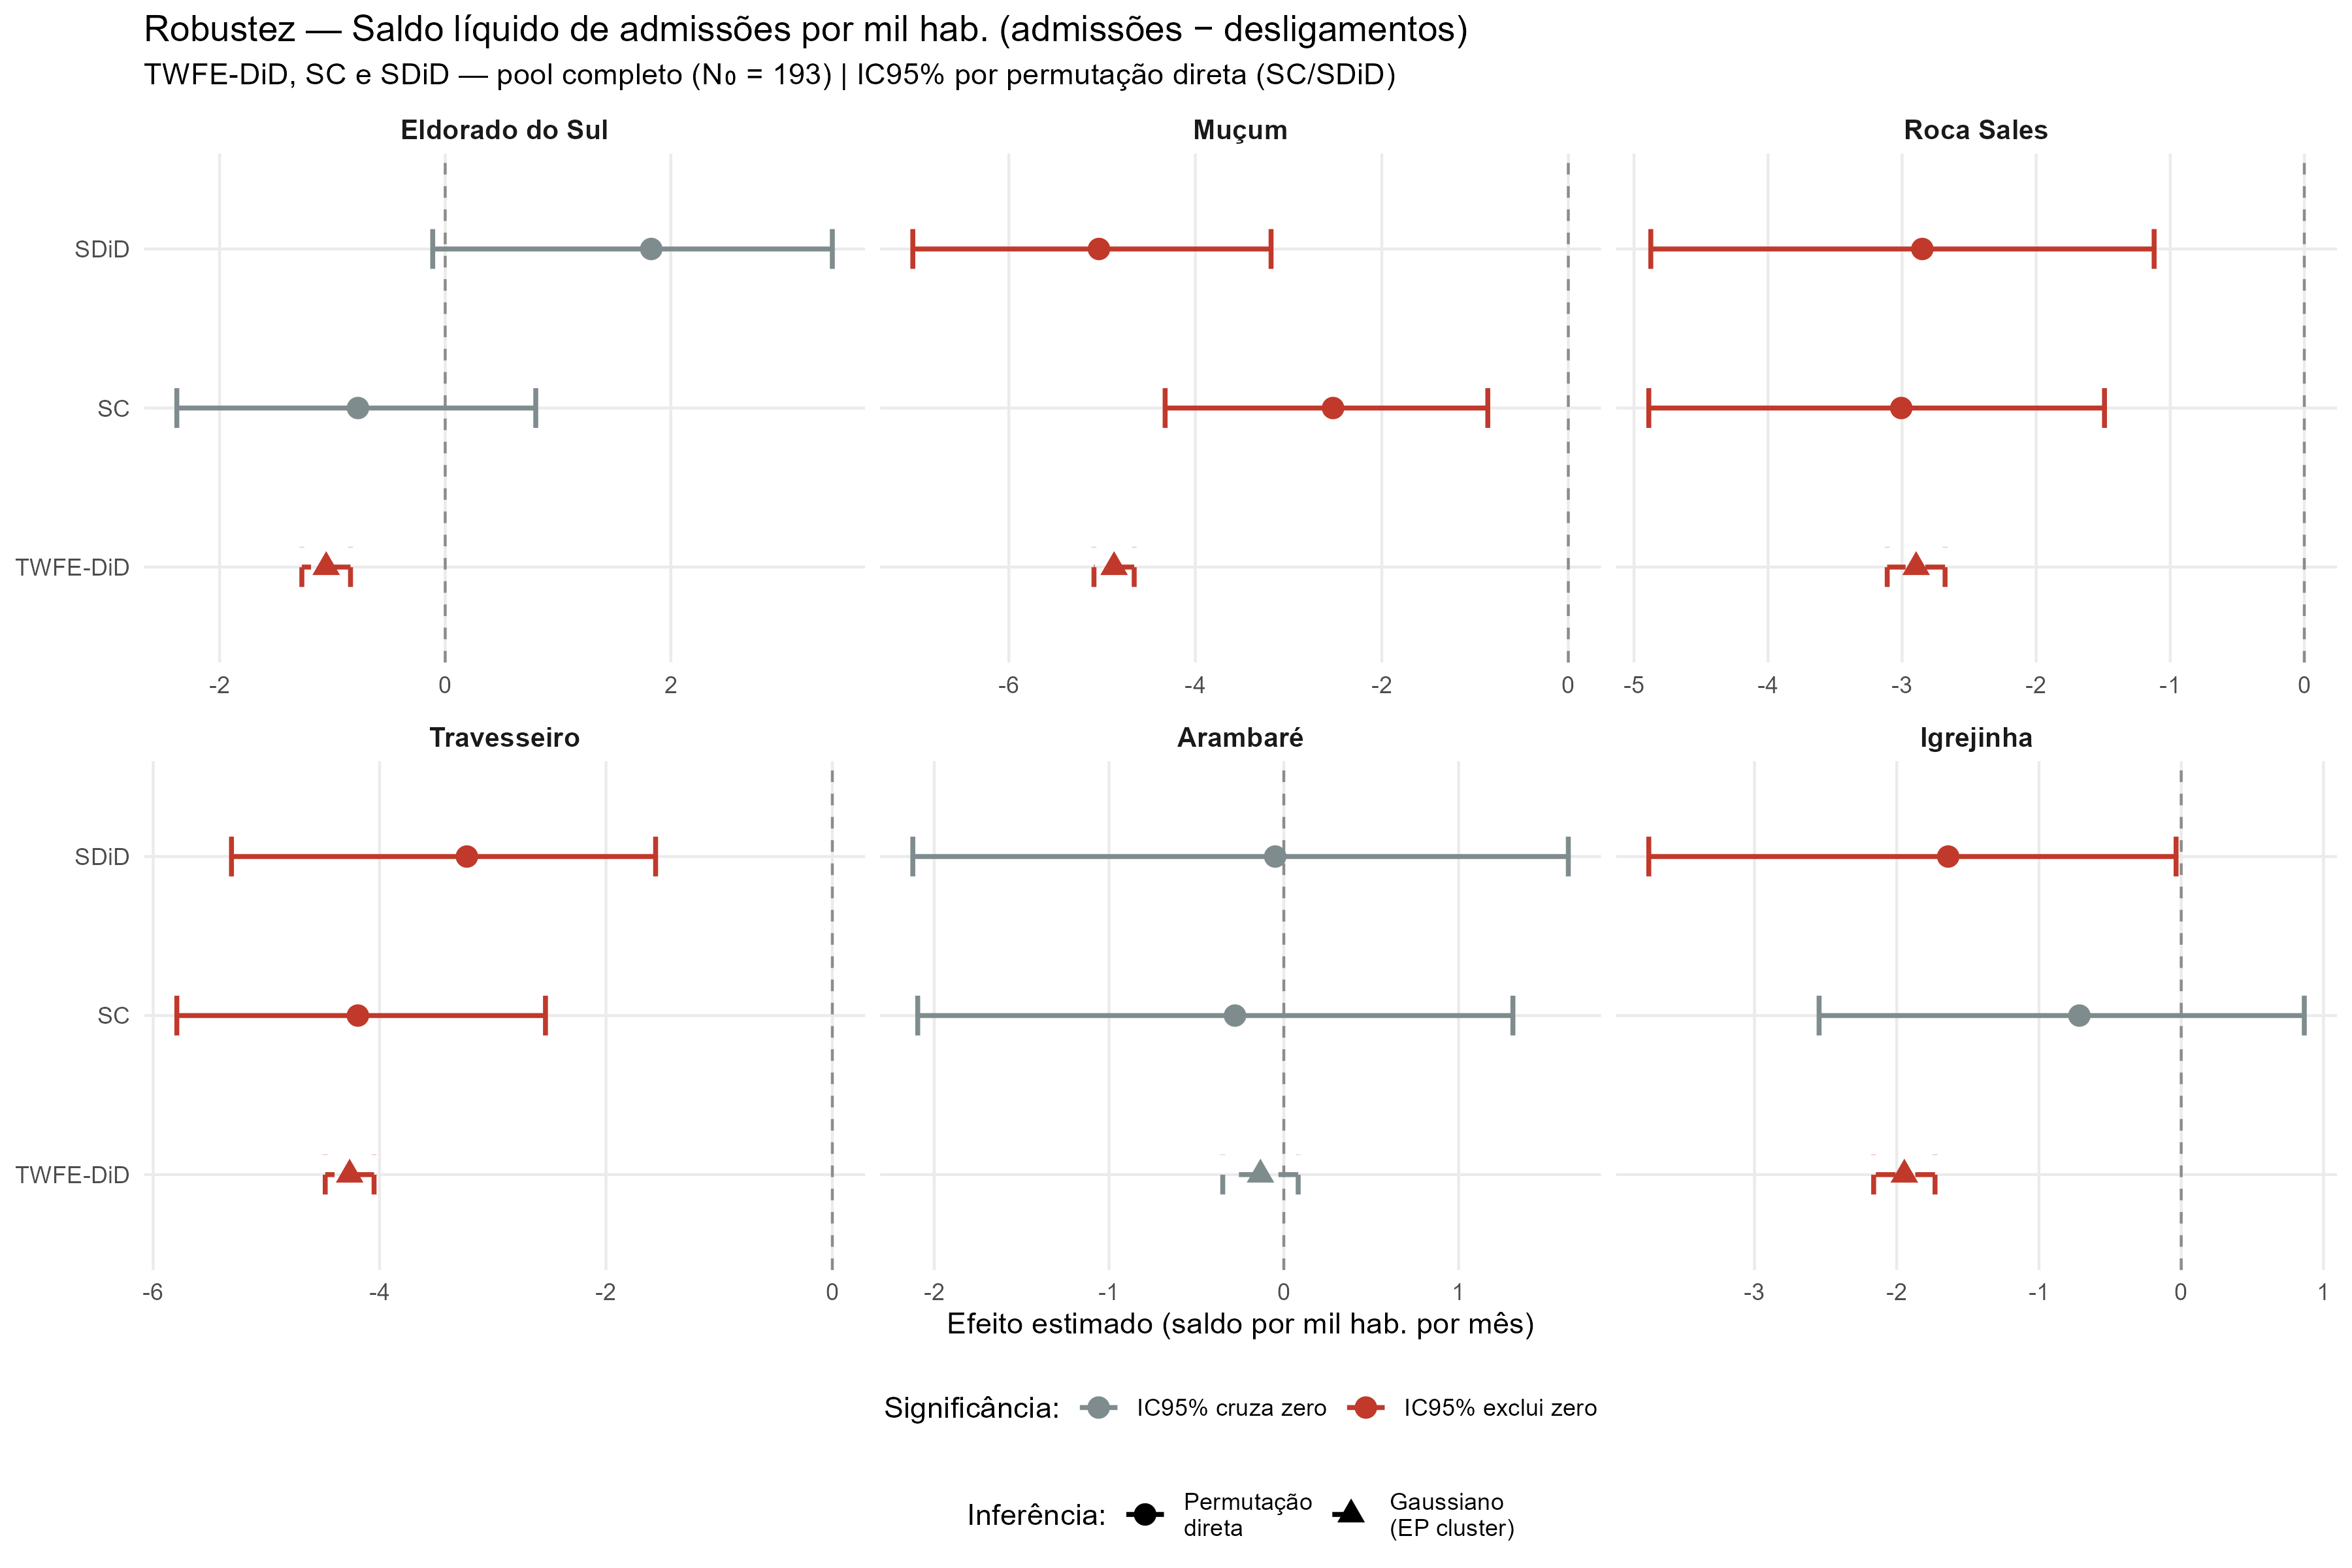
\includegraphics[width=0.95\textwidth]{triangulacao_saldo_forest.png}
\caption{\textit{Forest plot} da triangulação: saldo líquido de admissões por mil hab.
(TWFE-DiD, SC e SDiD; pool completo, $N_0 = 193$). Pontos vermelhos indicam IC95\%
inteiramente negativo (ou positivo); cinzas indicam IC que cruza zero. Inferência:
permutação direta para SC e SDiD; gaussiana para TWFE-DiD.}
\label{fig:forest_saldo}
\end{figure}

\begin{figure}[htbp]
\centering
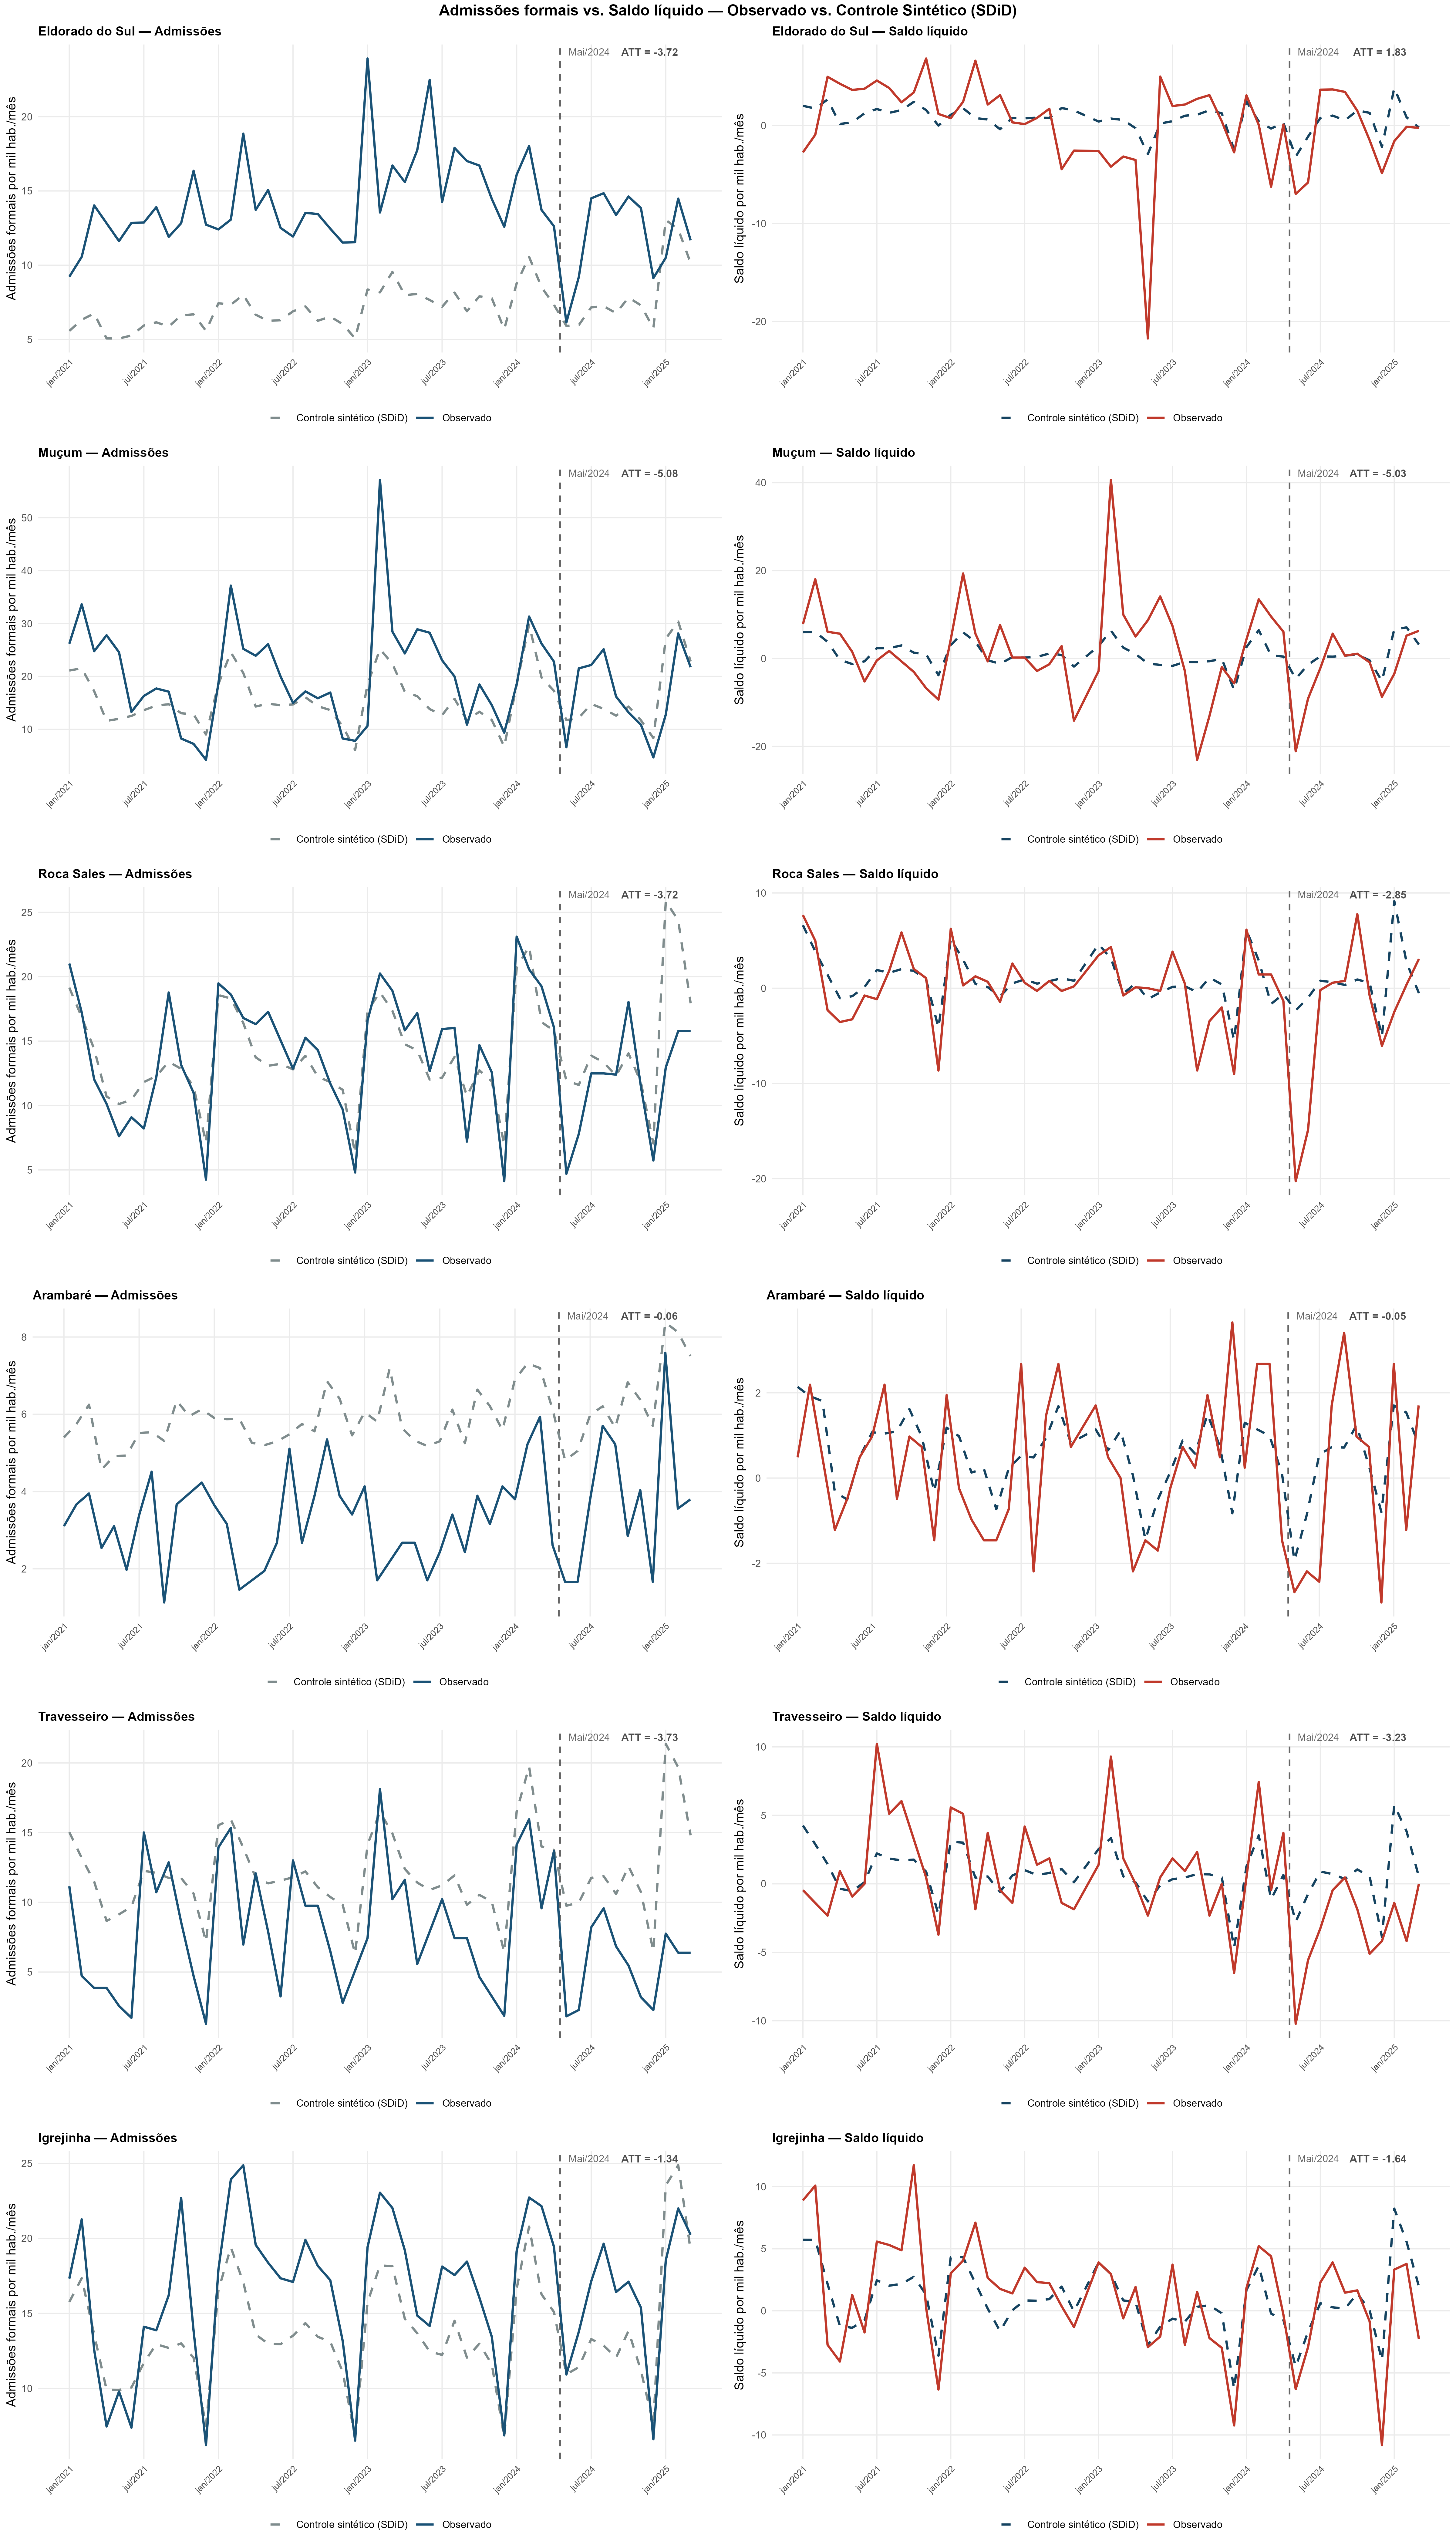
\includegraphics[width=\textwidth]{painel_admissoes_vs_saldo.png}
\caption{Trajetórias observada e controle sintético (SDiD) para admissões formais
(esquerda) e saldo líquido (direita), por município tratado. Linha vertical tracejada:
maio/2024. A convergência entre as duas séries no período pré-evento ilustra a qualidade
do ajuste do controle sintético; a divergência após mai/2024 captura o efeito estimado.}
\label{fig:painel_adm_saldo}
\end{figure}

% =============================================================
\clearpage
\section{Trajetórias expandidas do SDiD: admissões formais por município}
\label{apx:trajetorias}

Esta seção apresenta as trajetórias individuais entre a série observada e o controle
sintético SDiD para as admissões formais por mil habitantes em escala ampliada,
complementando a Figura~\ref{fig:trajetorias_todos} do texto principal. Para cada
município, a linha vermelha representa a série observada e a linha azul tracejada
o controle sintético estimado; a linha vertical cinza indica maio de 2024 (início
do tratamento). A área sombreada inferior representa os pesos temporais ótimos
$\hat{\lambda}_t$, que o SDiD concentra nos meses imediatamente anteriores ao
evento \cite{arkhangelsky2021}. Os $p$-valores são bilaterais por permutação direta.

% ── Par 1: Eldorado do Sul + Muçum ───────────────────────────
\begin{figure}[htbp]
\centering
\subcaptionbox{Eldorado do Sul: ATT\,$=-3{,}72$; IC95\%\,$[-7{,}04;\,-0{,}52]$; $p=0{,}041$\label{subfig:bex_es}}
  [0.47\textwidth]{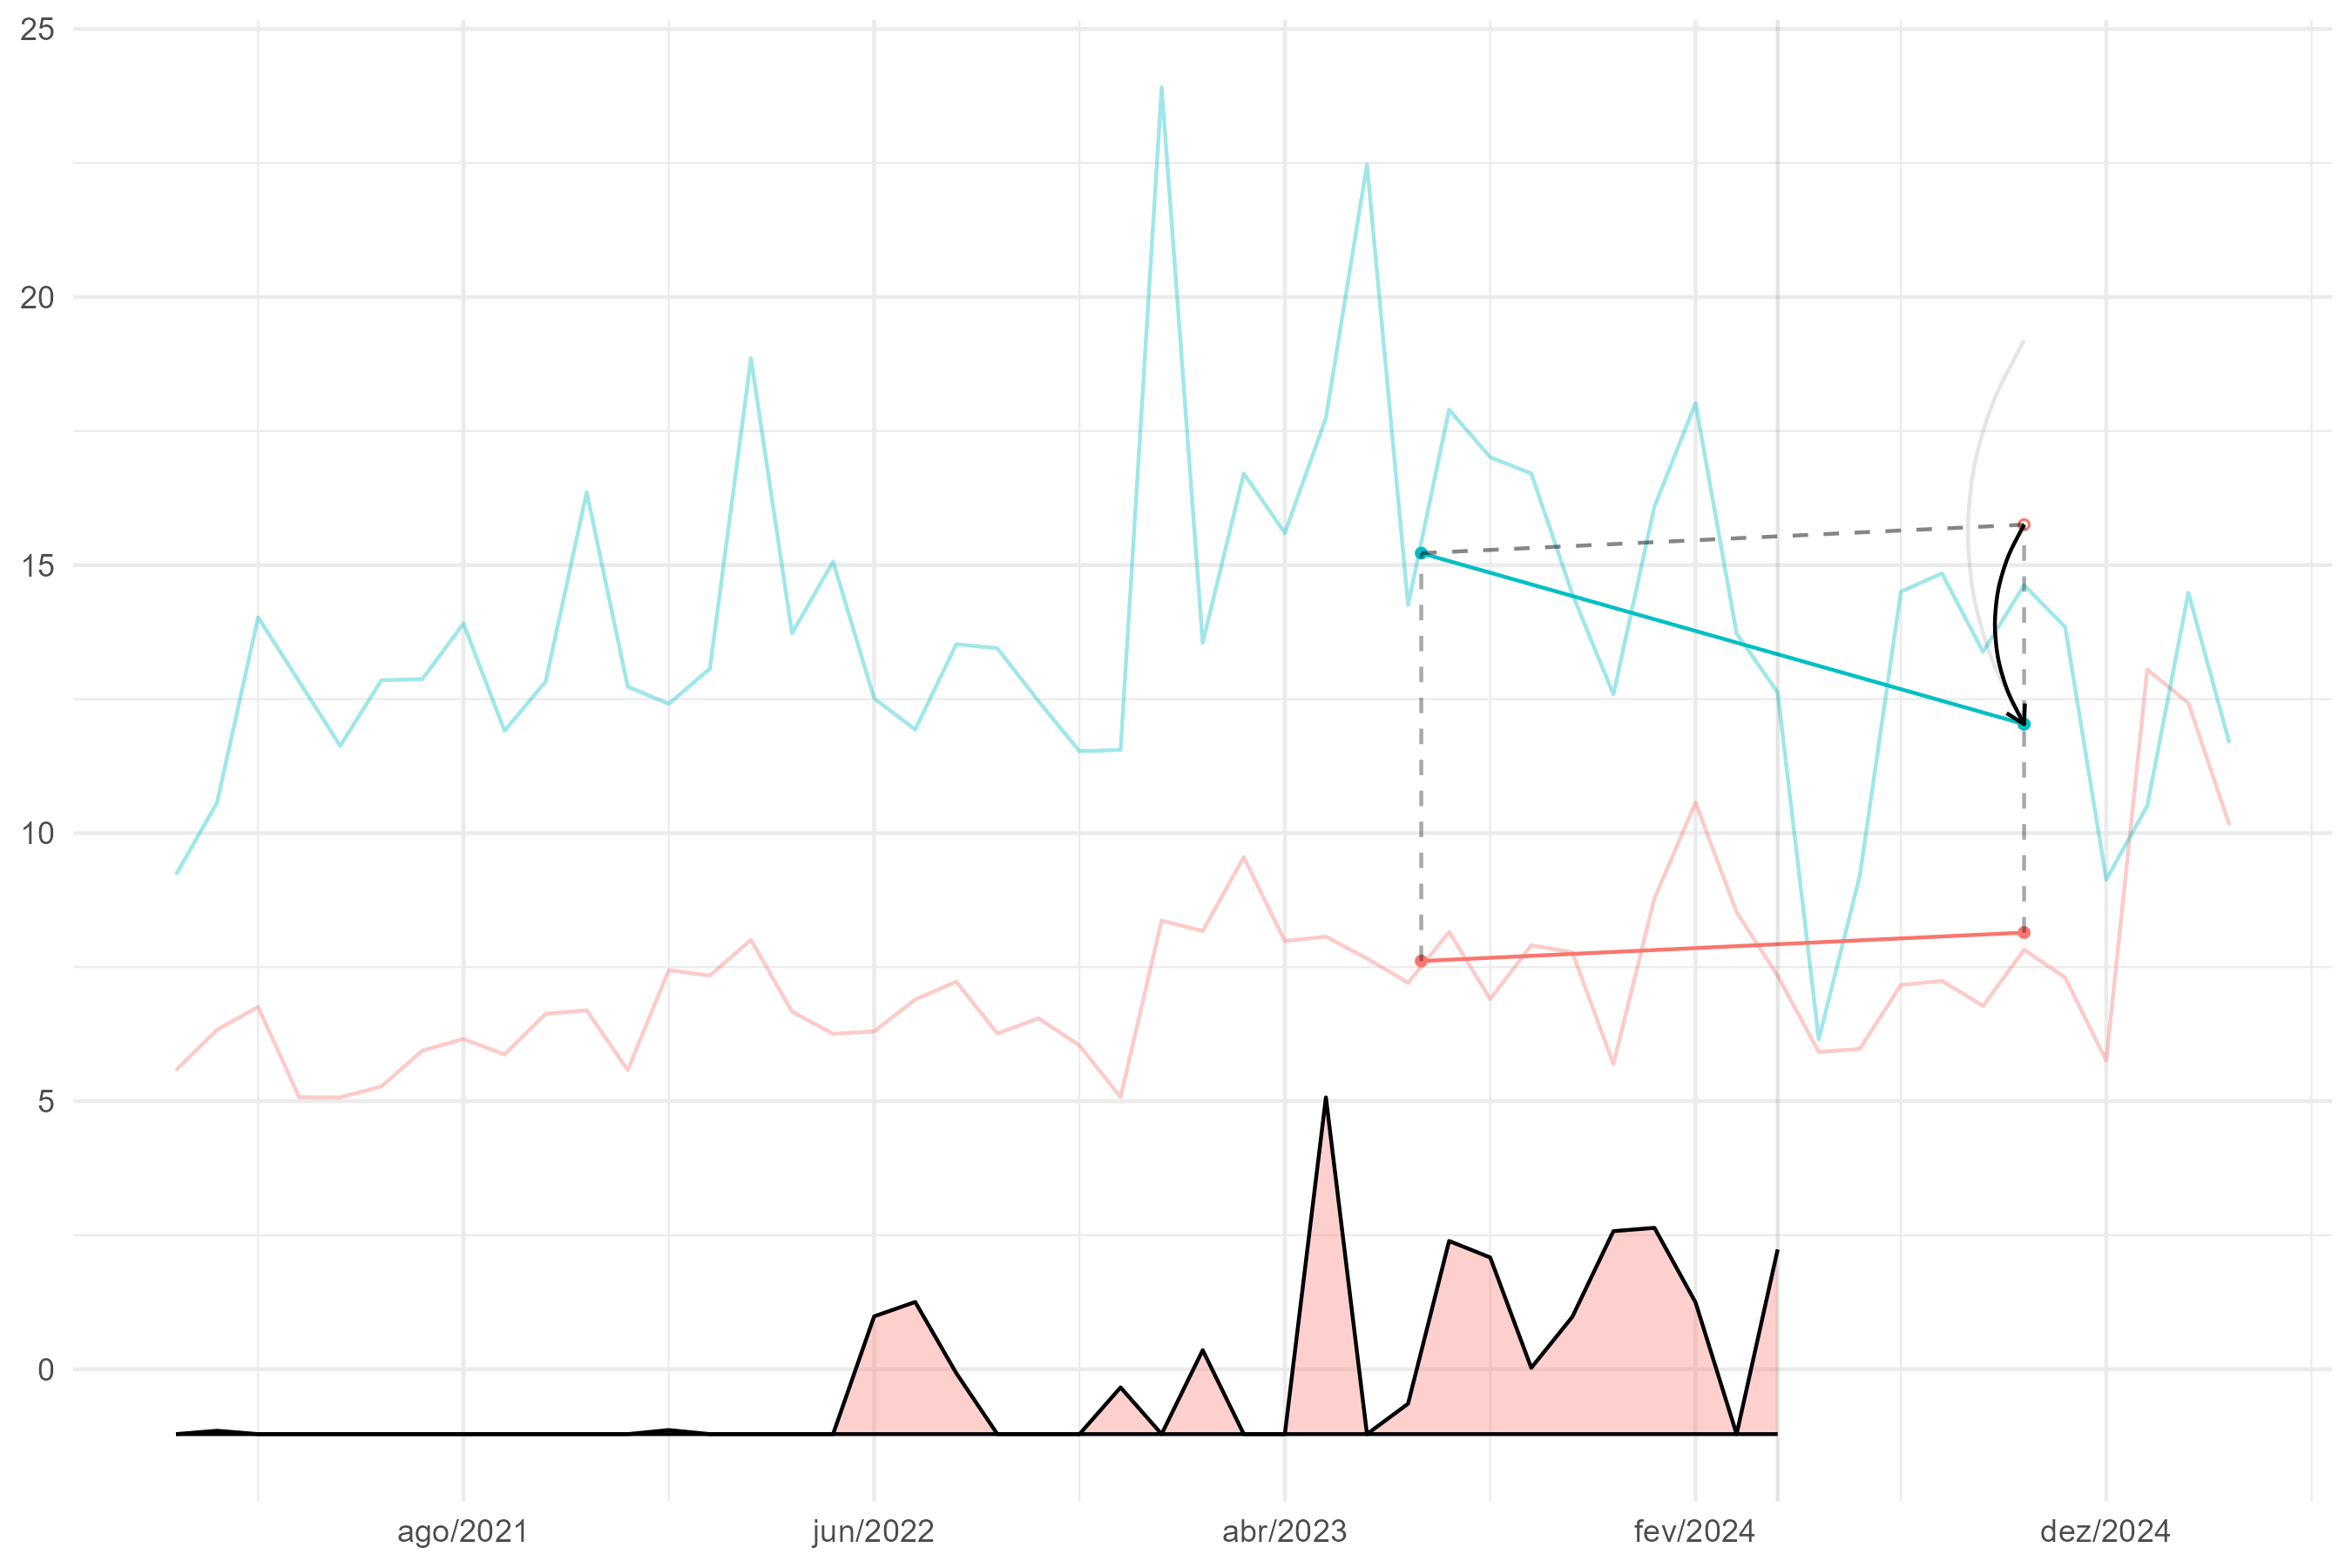
\includegraphics[width=0.47\textwidth]{municipio_4306767_completo_trajetorias.png}}
\hfill
\subcaptionbox{Mu\c{c}um$^{\dagger}$: ATT\,$=-5{,}08$; IC95\%\,$[-7{,}74;\,-2{,}17]$; $p=0{,}016$\label{subfig:bex_mucum}}
  [0.47\textwidth]{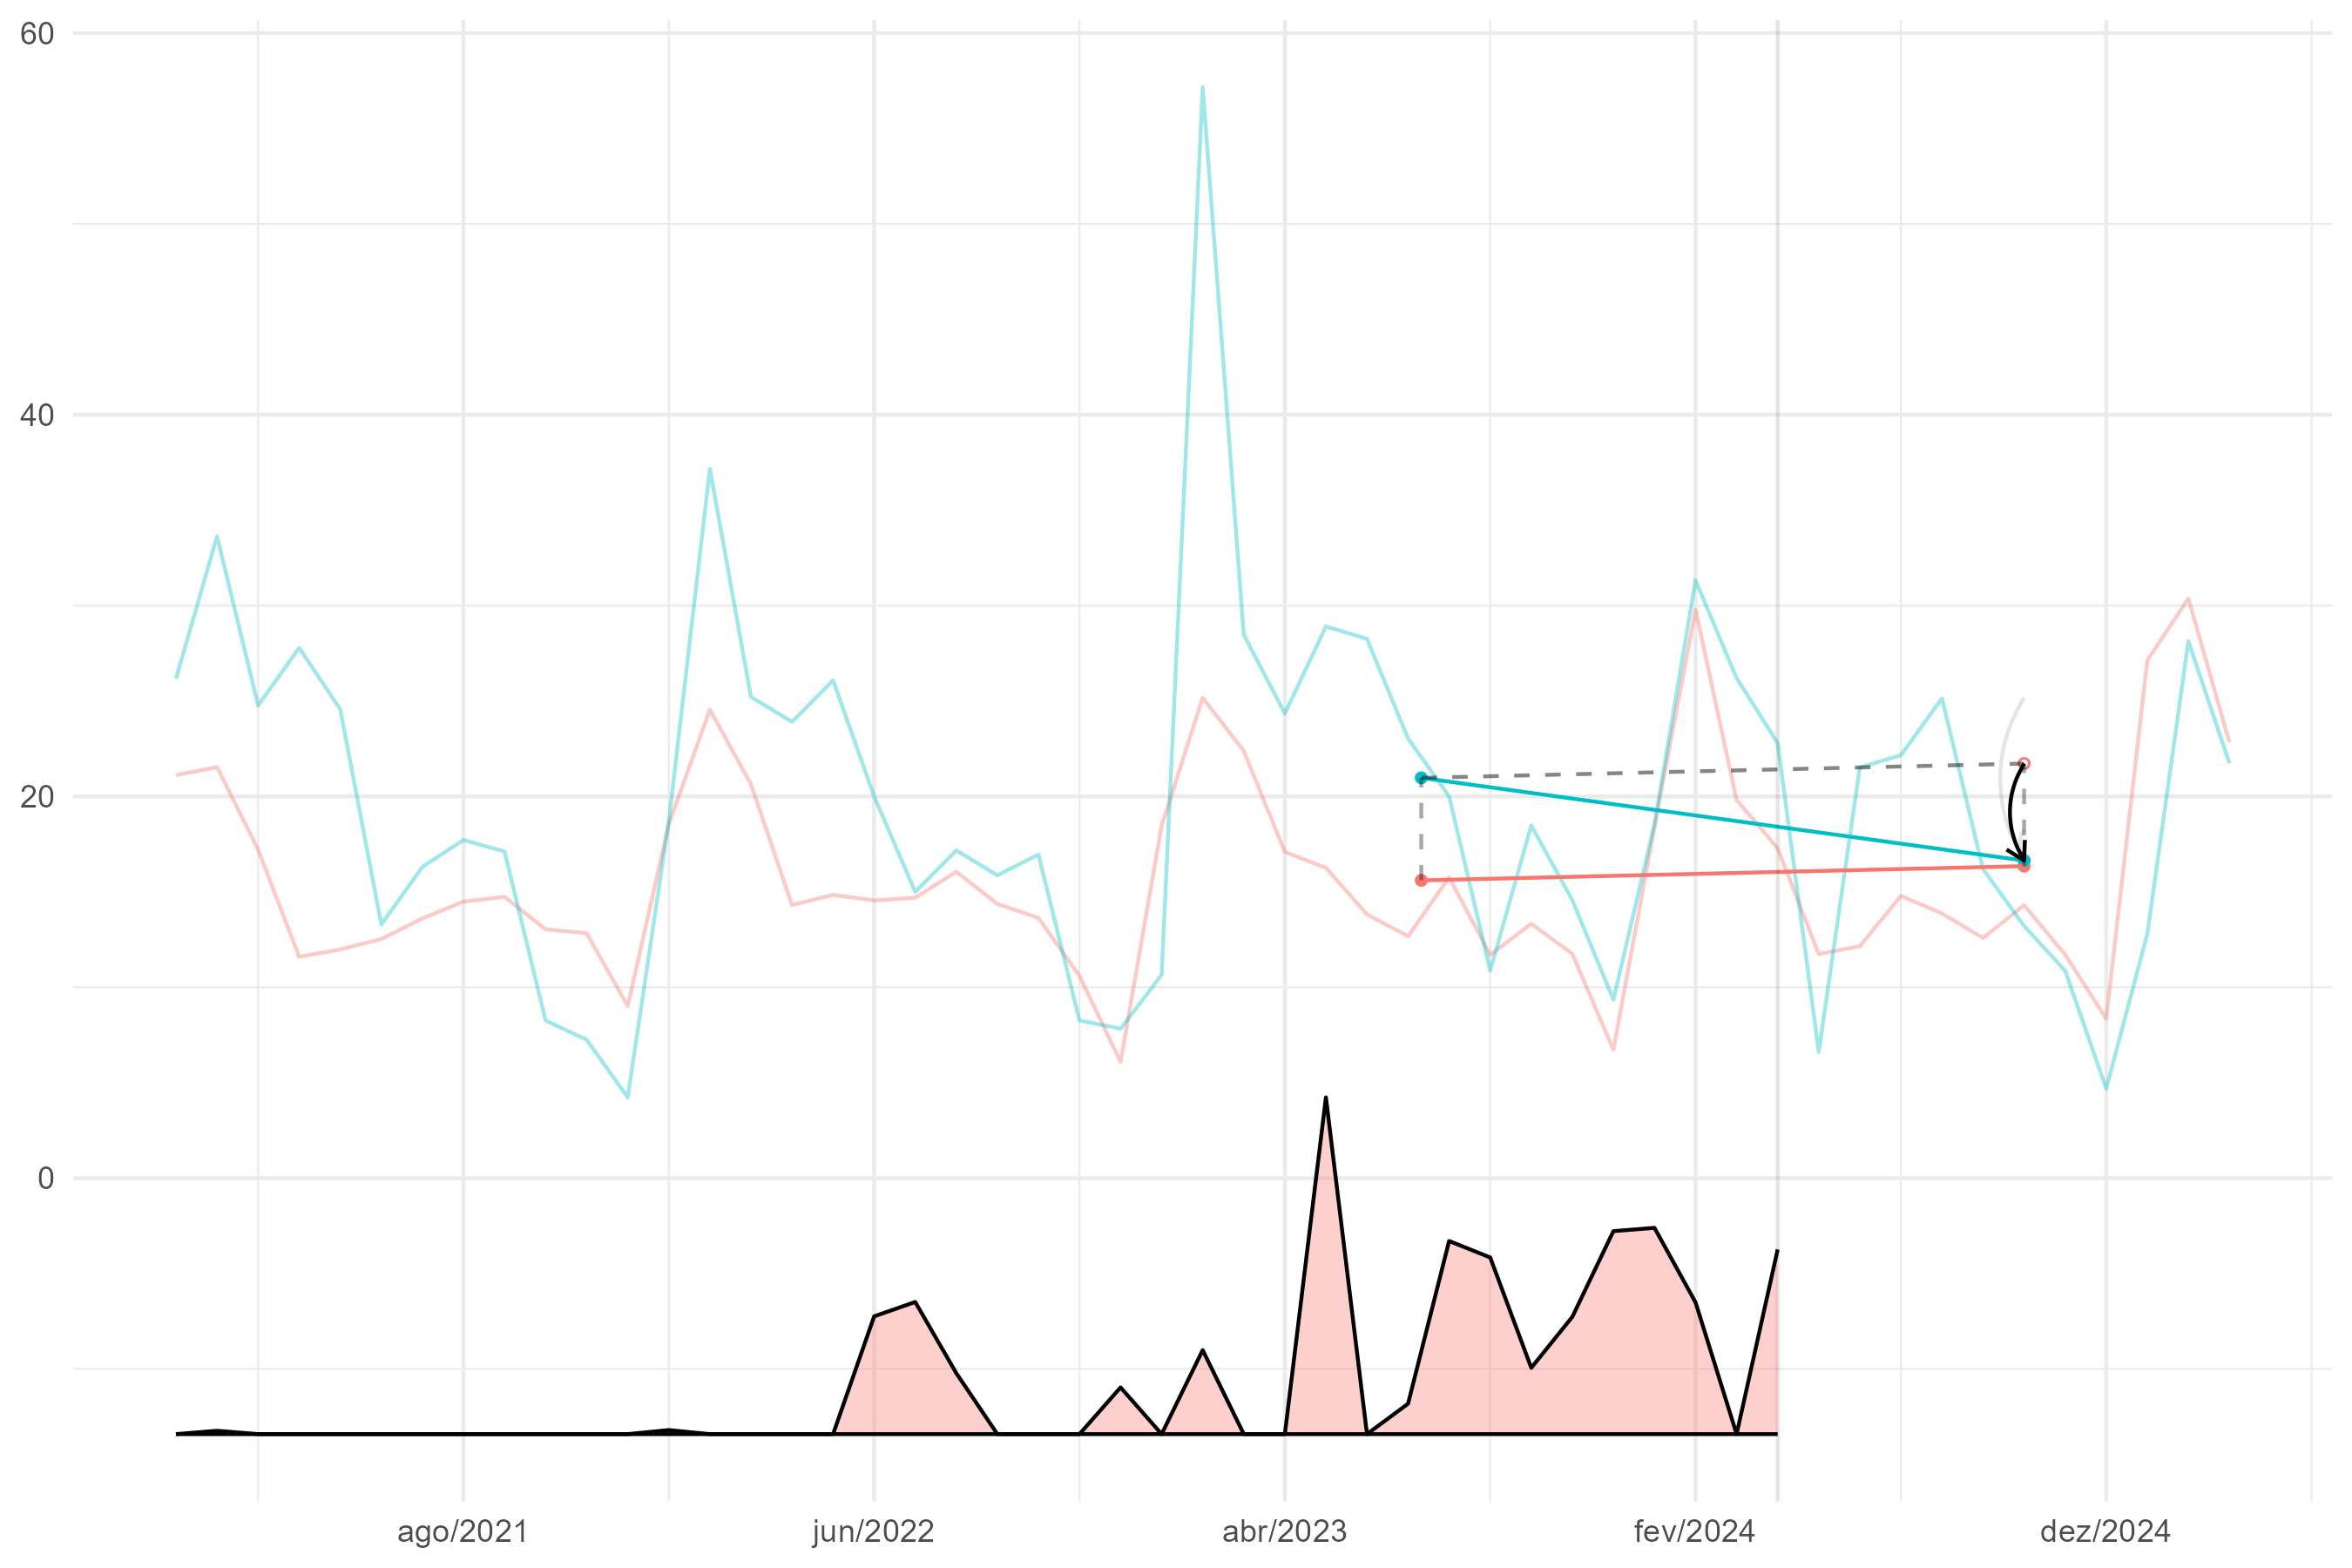
\includegraphics[width=0.47\textwidth]{municipio_4312609_completo_trajetorias.png}}
\caption{Trajetórias expandidas (1/3): municípios Eldorado do Sul e Muçum. $^{\dagger}$RMSPE\,pré\,$>5{,}0$ (inferência parcial). Pool completo, $N_0=193$. Fonte: elaboração própria.}
\label{fig:bex_par1}
\end{figure}

% ── Par 2: Roca Sales + Travesseiro ──────────────────────────
\begin{figure}[htbp]
\centering
\subcaptionbox{Roca Sales: ATT\,$=-3{,}72$; IC95\%\,$[-6{,}37;\,-0{,}58]$; $p=0{,}036$\label{subfig:bex_rs}}
  [0.47\textwidth]{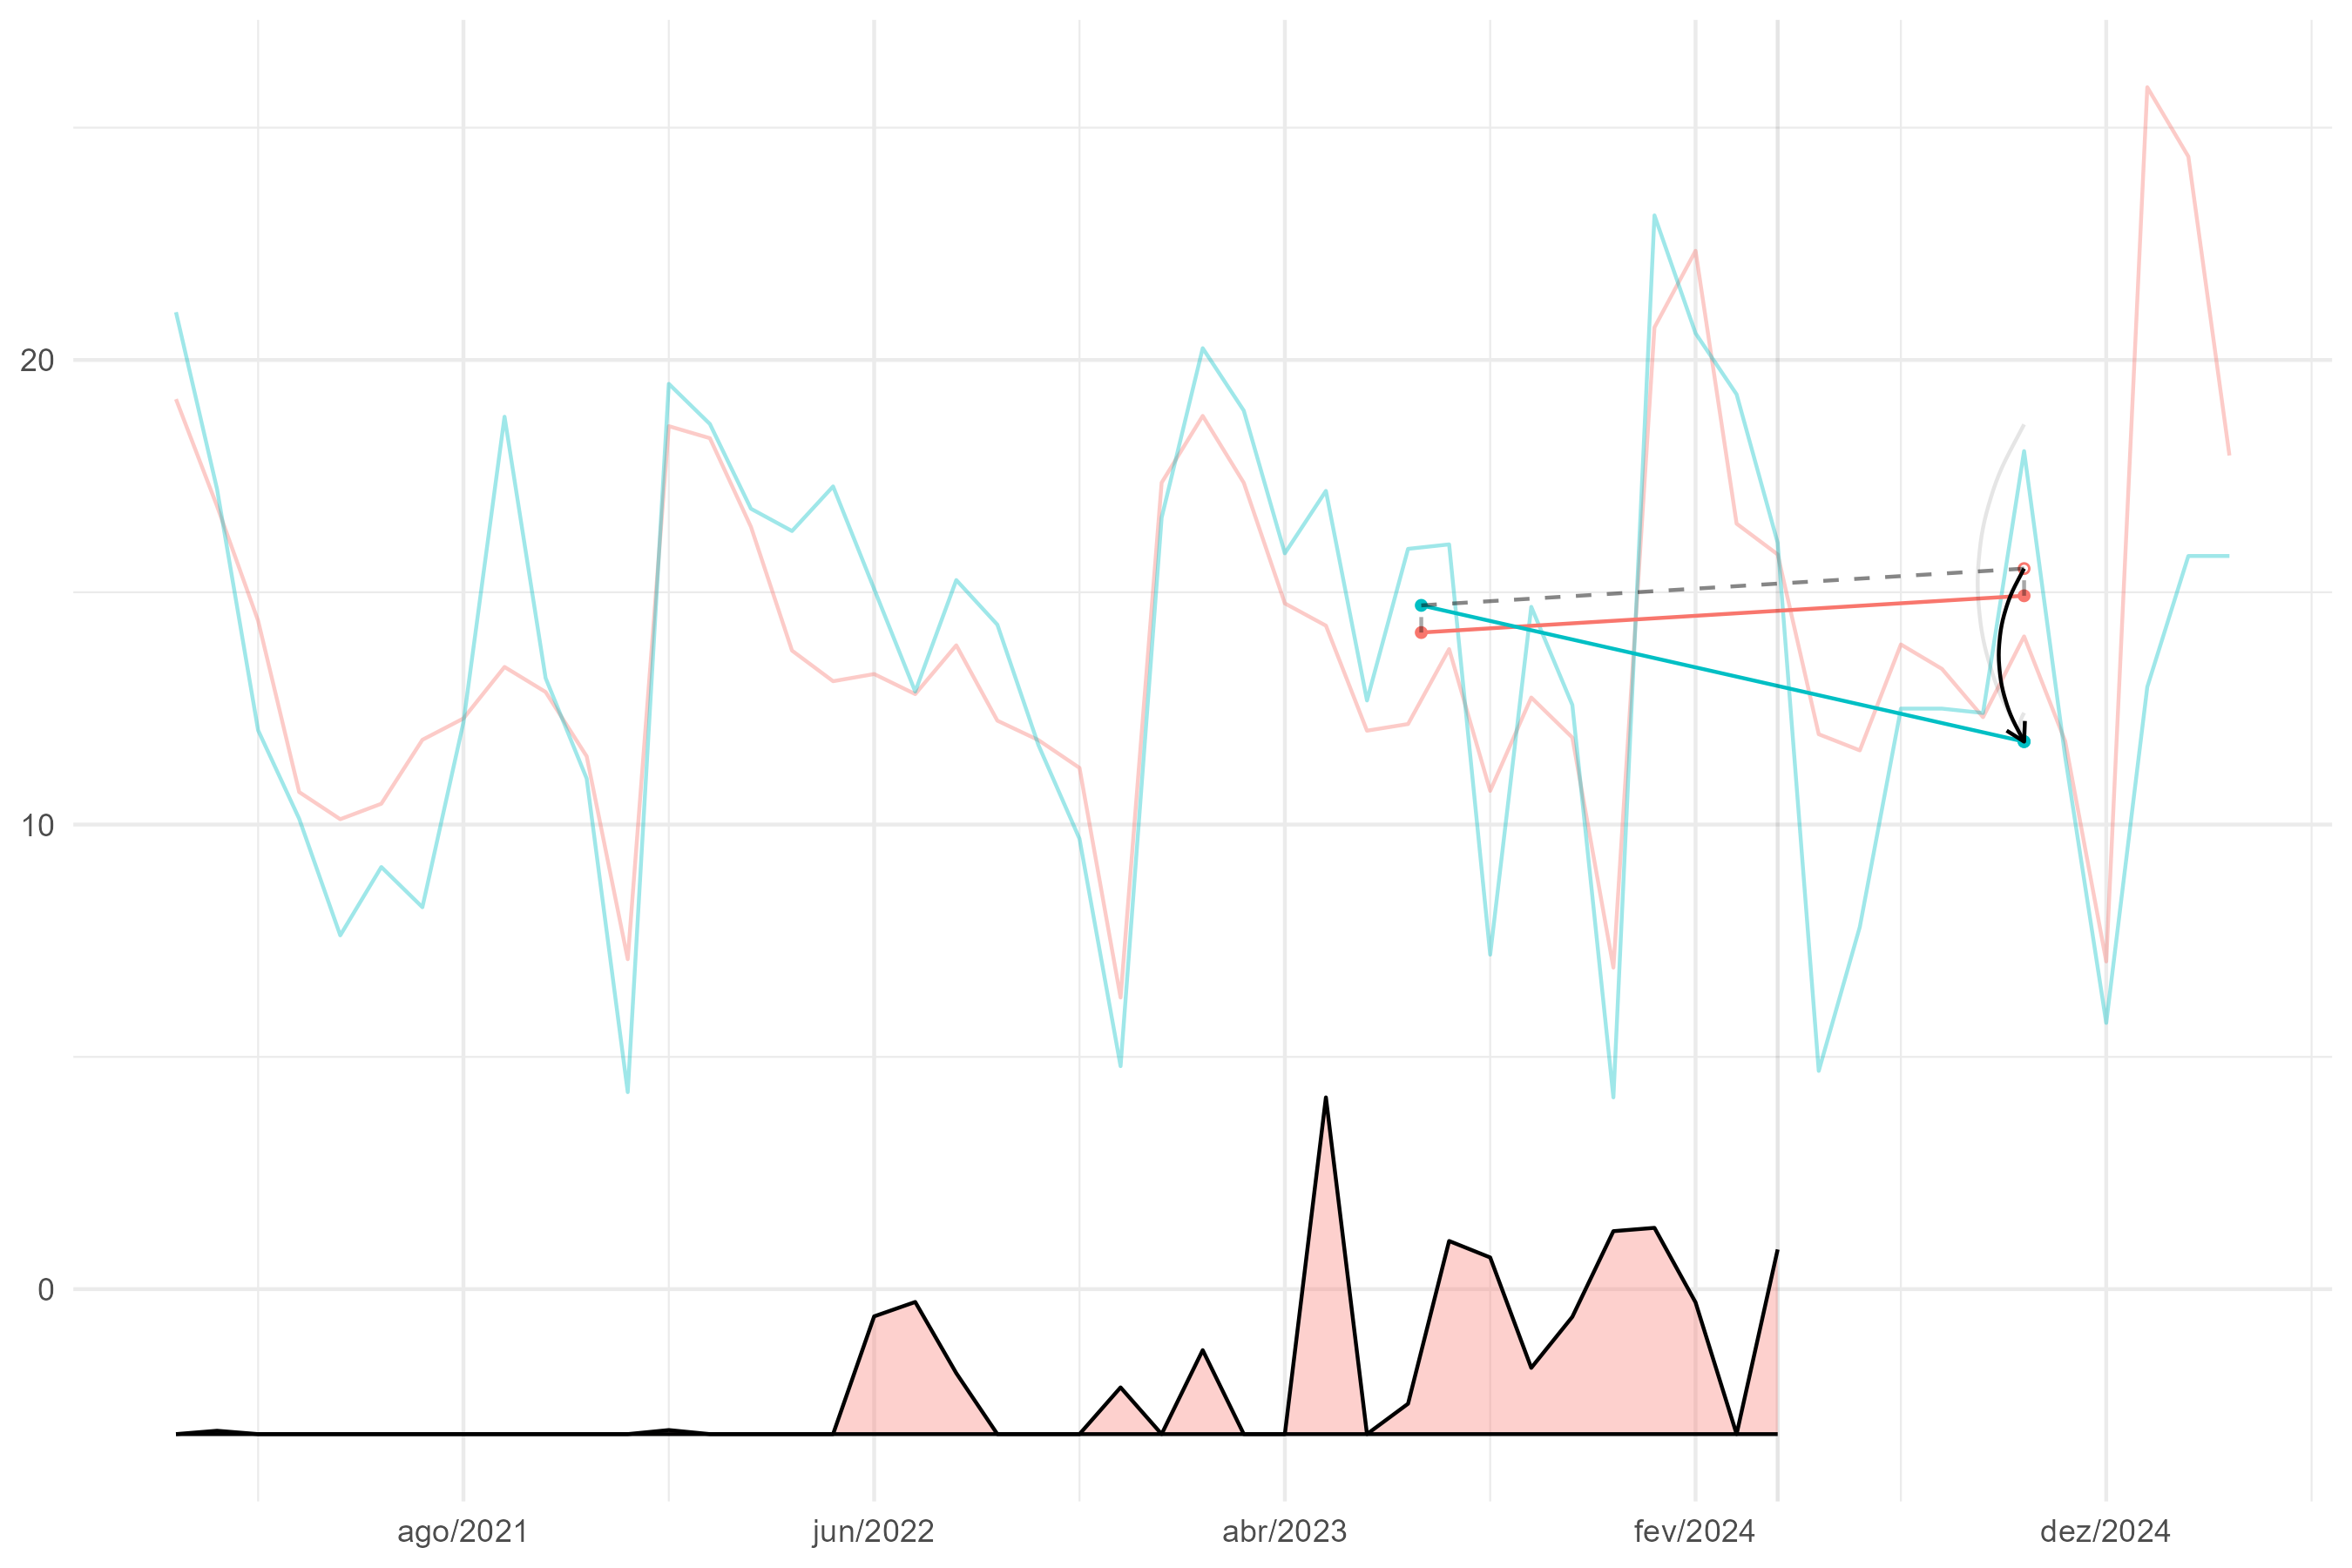
\includegraphics[width=0.47\textwidth]{municipio_4315800_completo_trajetorias.png}}
\hfill
\subcaptionbox{Travesseiro: ATT\,$=-3{,}73$; IC95\%\,$[-7{,}11;\,-0{,}63]$; $p=0{,}036$\label{subfig:bex_trav}}
  [0.47\textwidth]{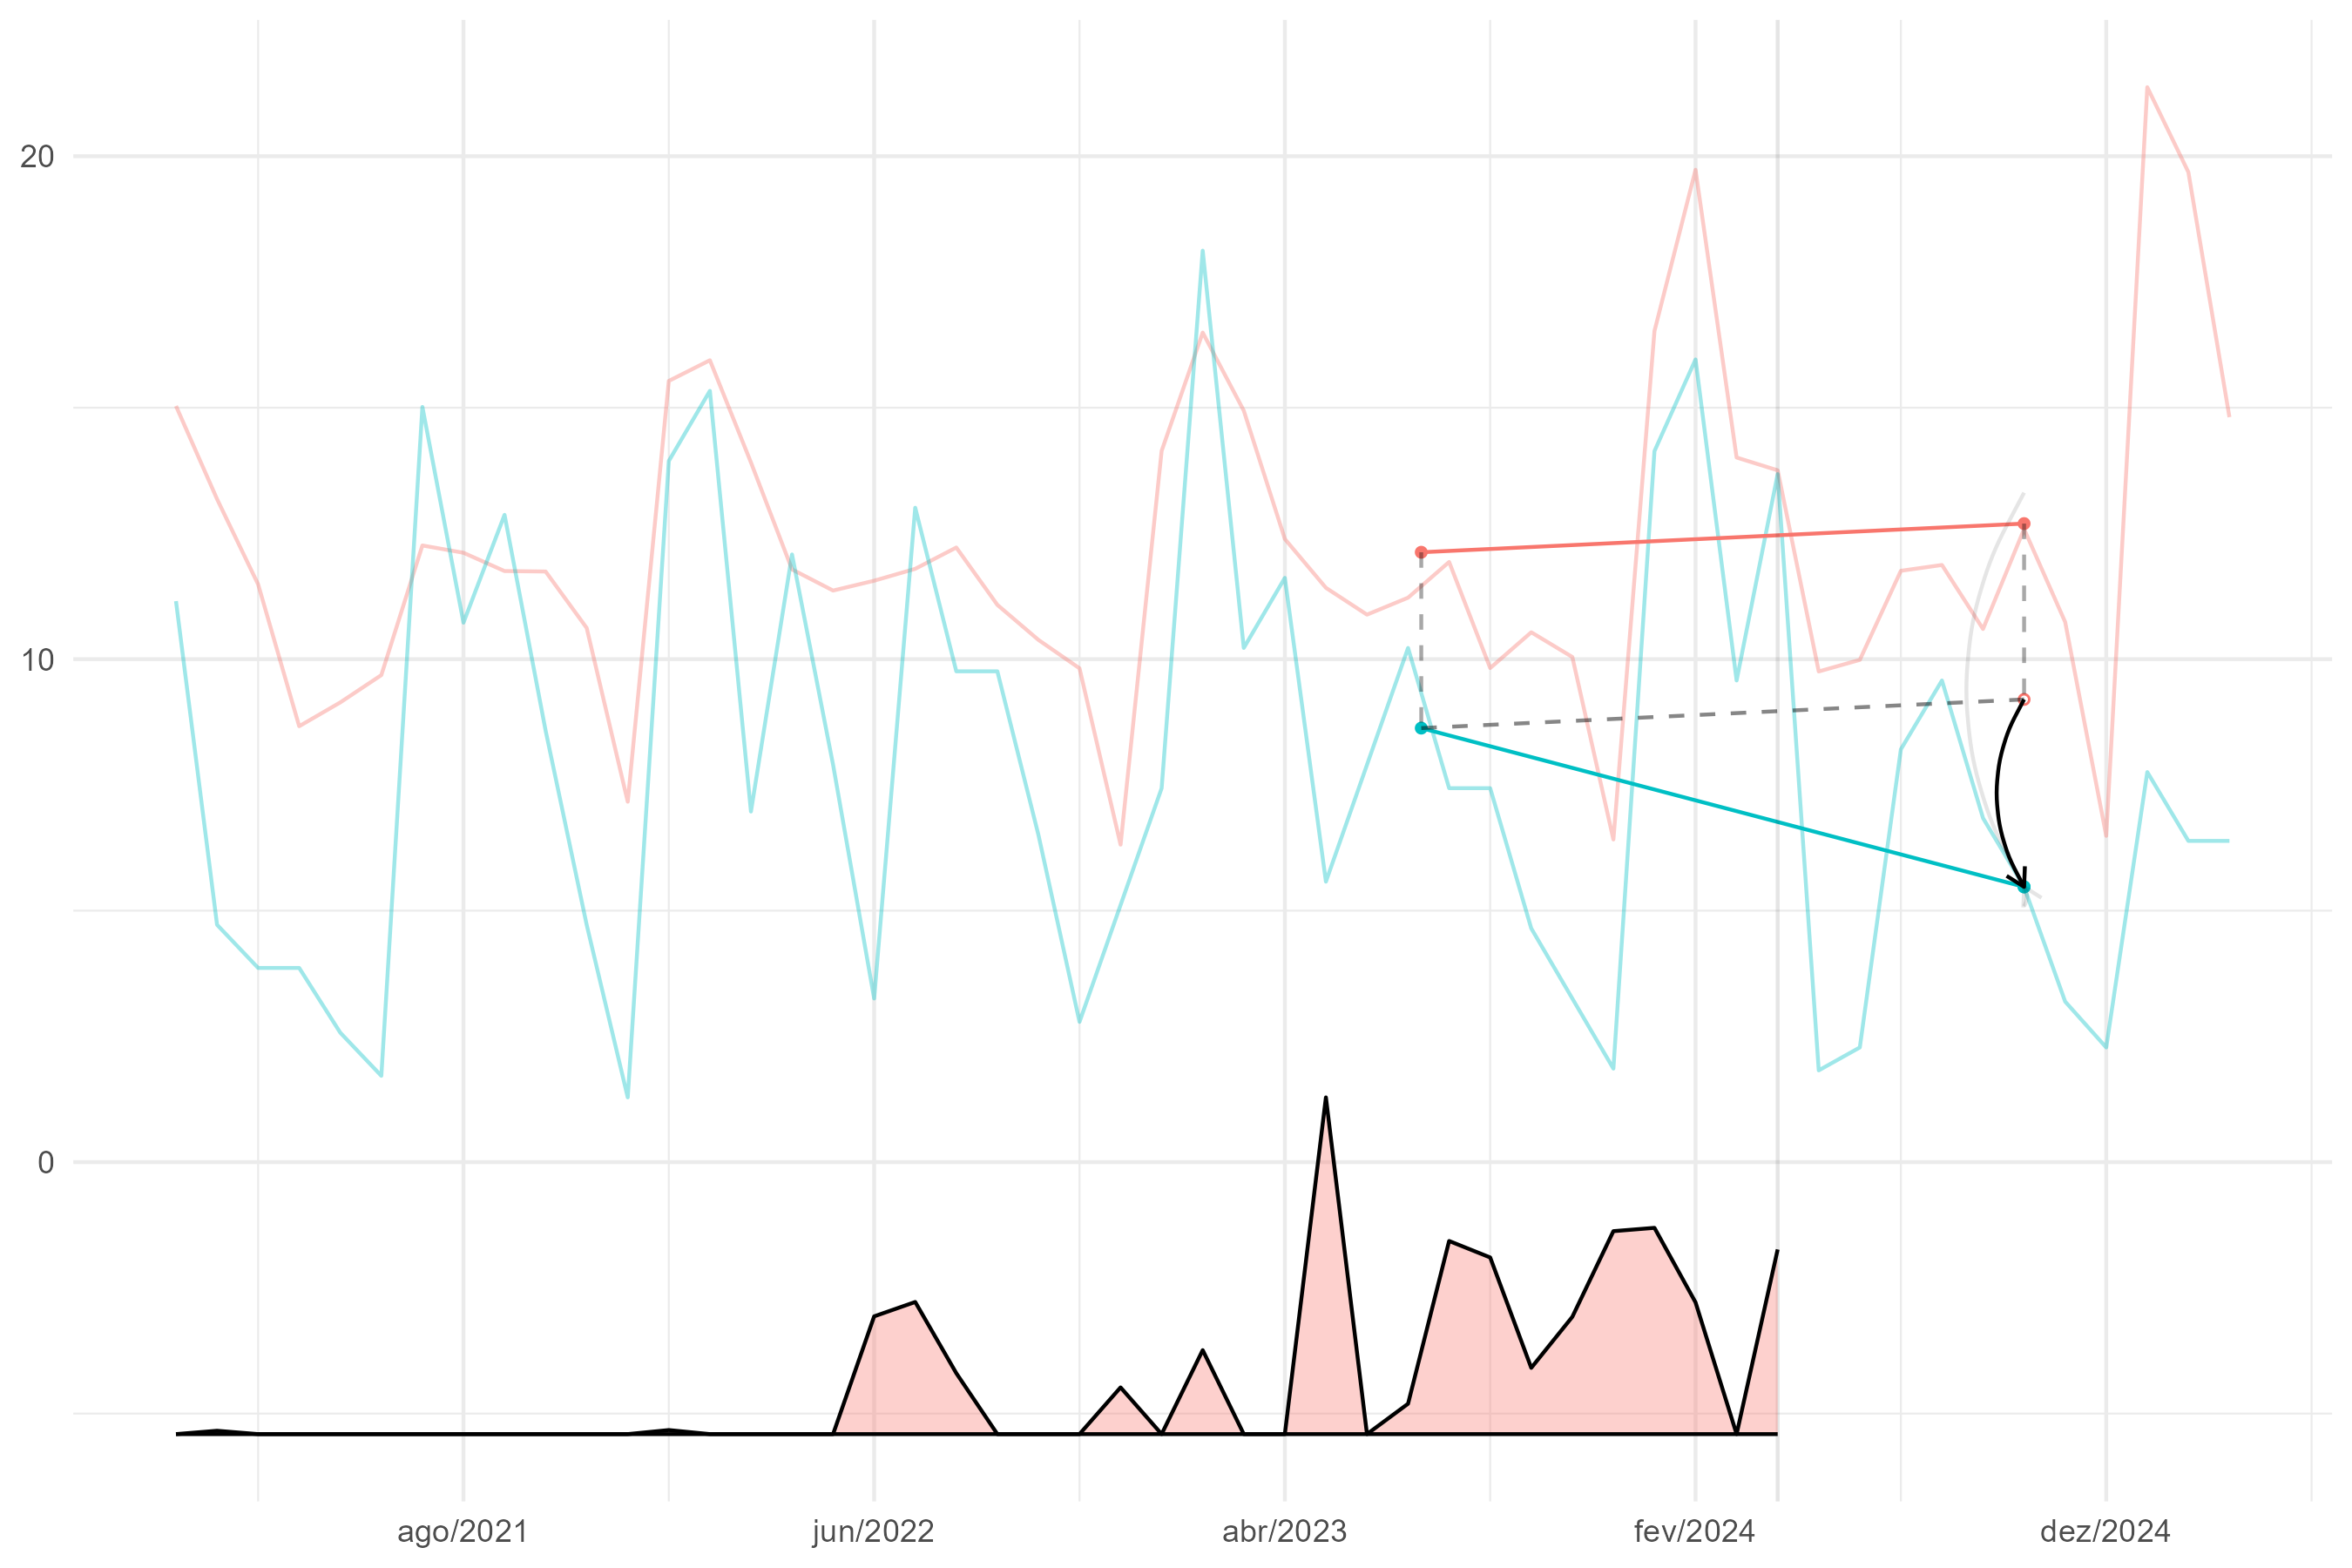
\includegraphics[width=0.47\textwidth]{municipio_4321626_completo_trajetorias.png}}
\caption{Trajetórias expandidas (2/3): municípios Roca Sales e Travesseiro. Efeito robusto em ambos: IC95\% inteiramente negativo e placebo no tempo $p=0{,}040$. Pool completo, $N_0=193$. Fonte: elaboração própria.}
\label{fig:bex_par2}
\end{figure}

% ── Par 3: Arambaré + Igrejinha ───────────────────────────────
\begin{figure}[htbp]
\centering
\subcaptionbox{Arambaré: ATT\,$=-0{,}06$; IC95\%\,$[-3{,}10;\,+3{,}03]$; $p=0{,}943$\label{subfig:bex_aram}}
  [0.47\textwidth]{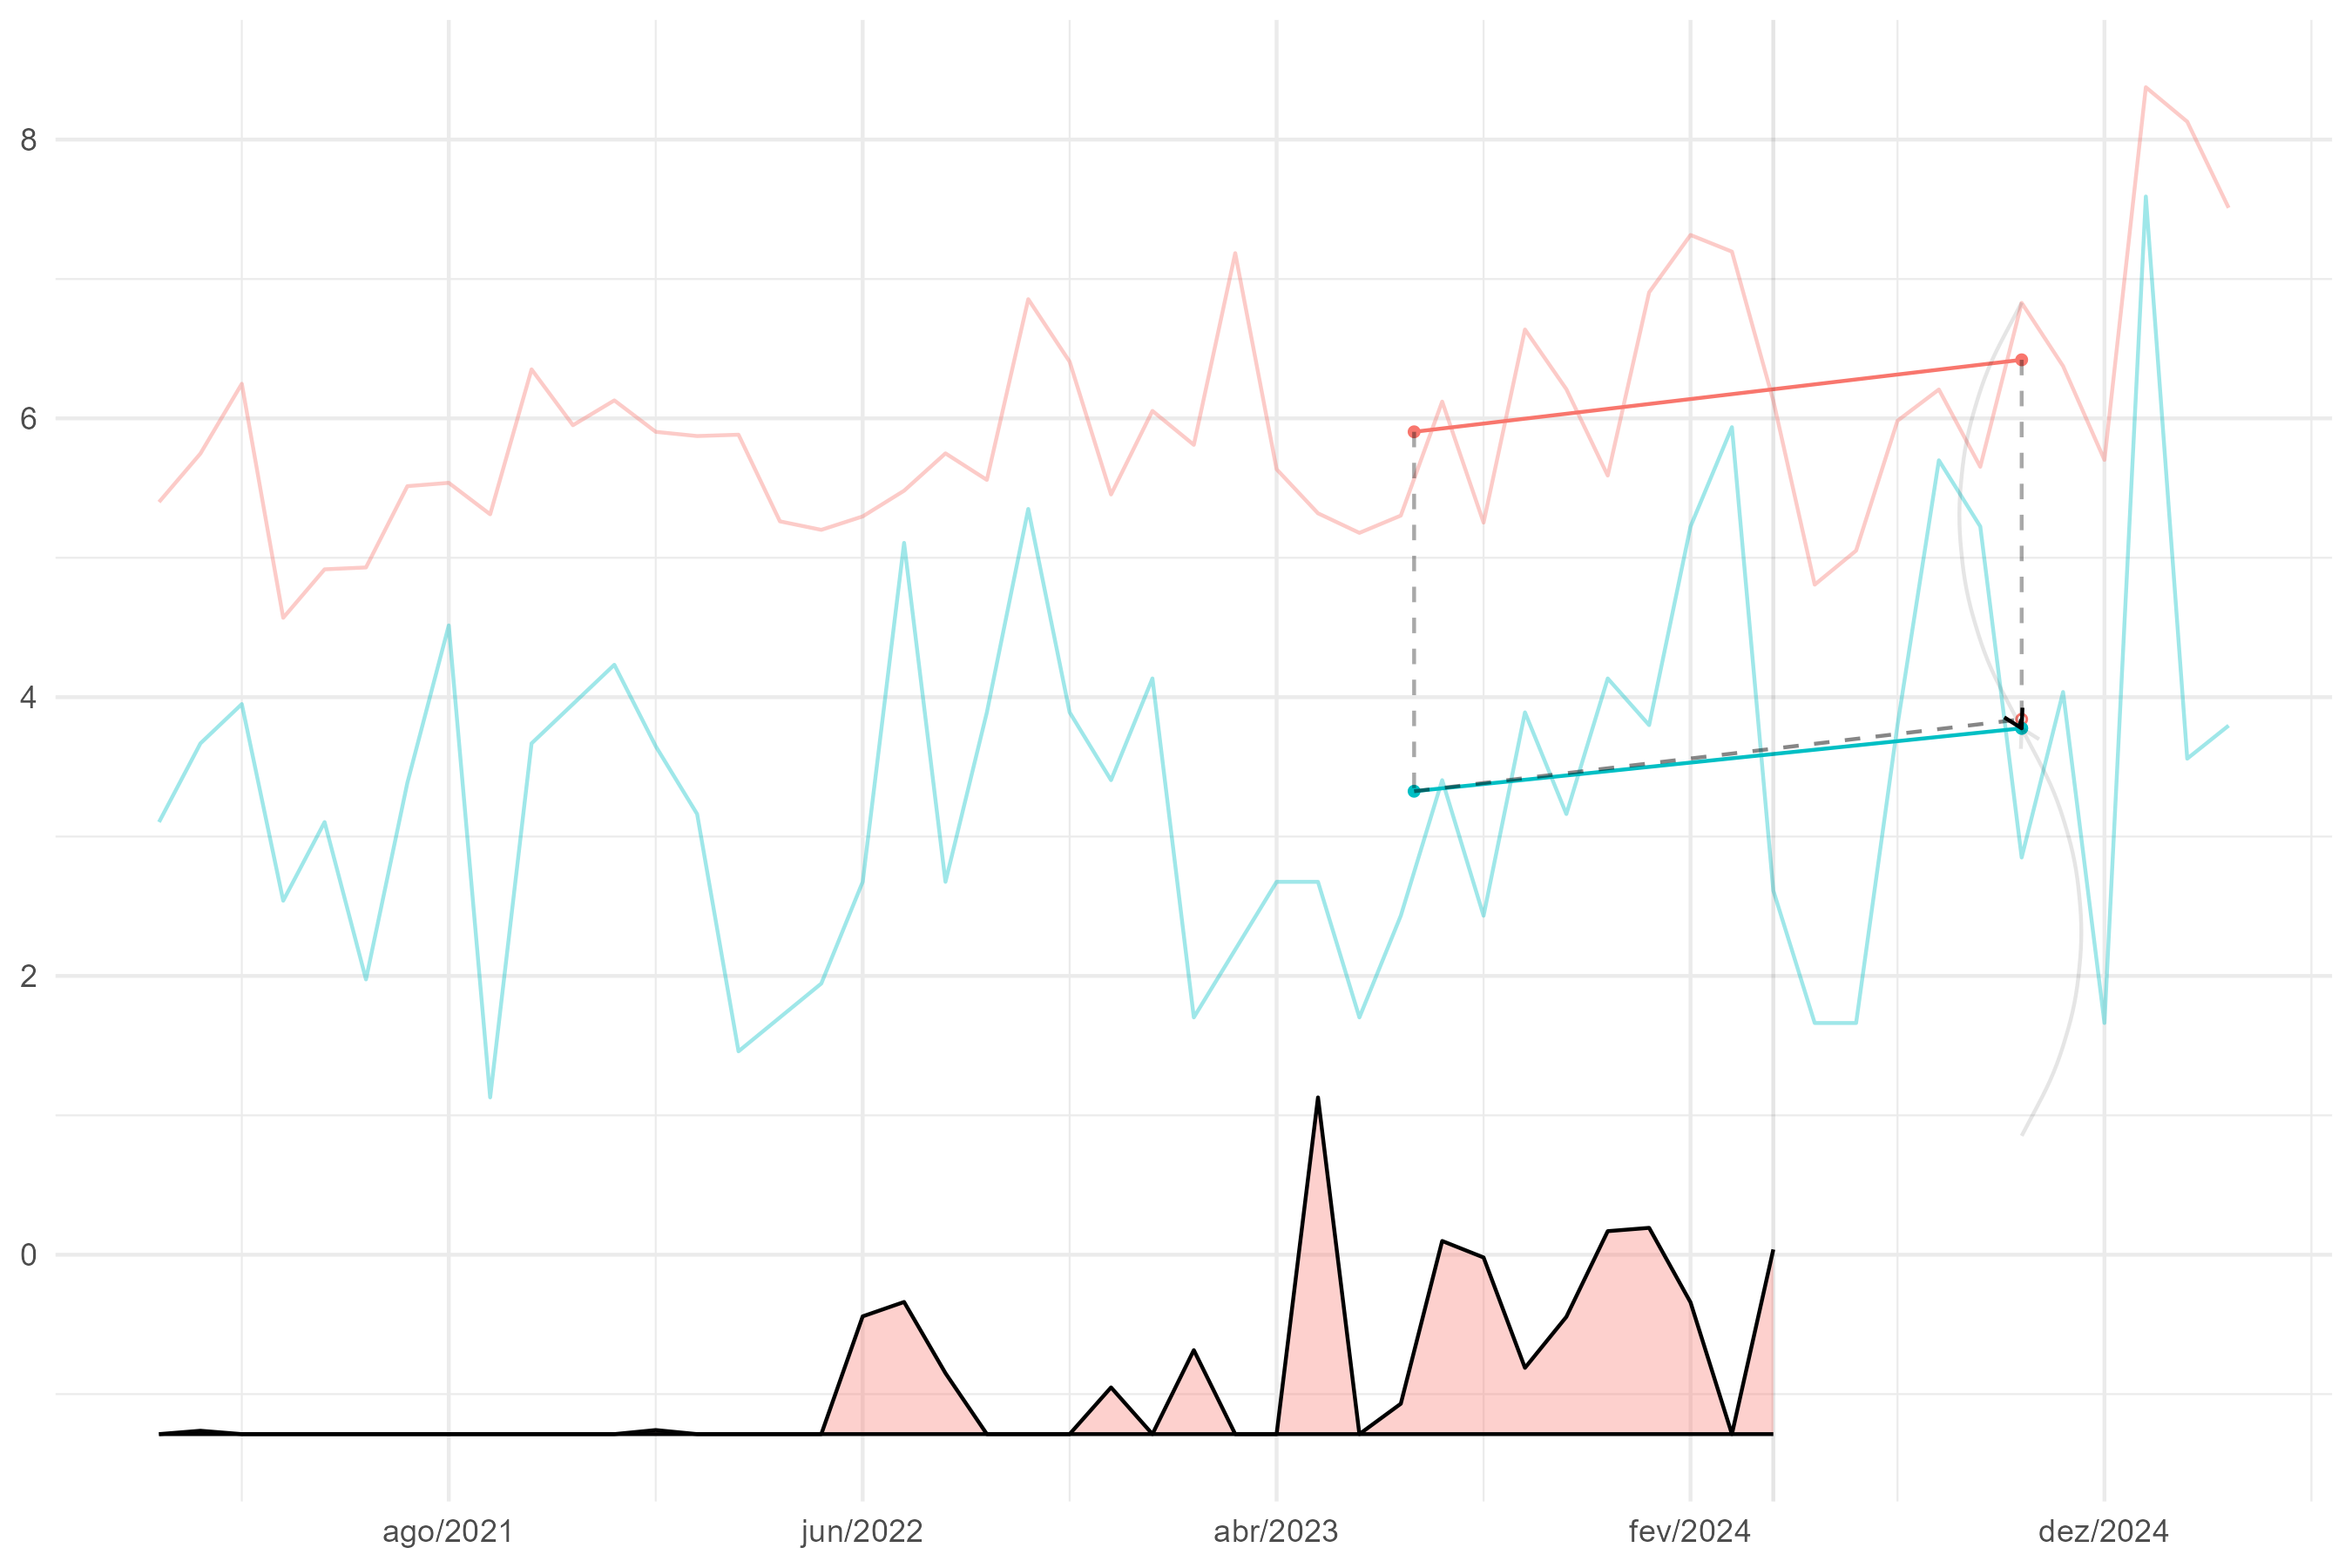
\includegraphics[width=0.47\textwidth]{municipio_4300851_completo_trajetorias.png}}
\hfill
\subcaptionbox{Igrejinha: ATT\,$=-1{,}34$; IC95\%\,$[-4{,}40;\,+1{,}78]$; $p=0{,}207$\label{subfig:bex_igrej}}
  [0.47\textwidth]{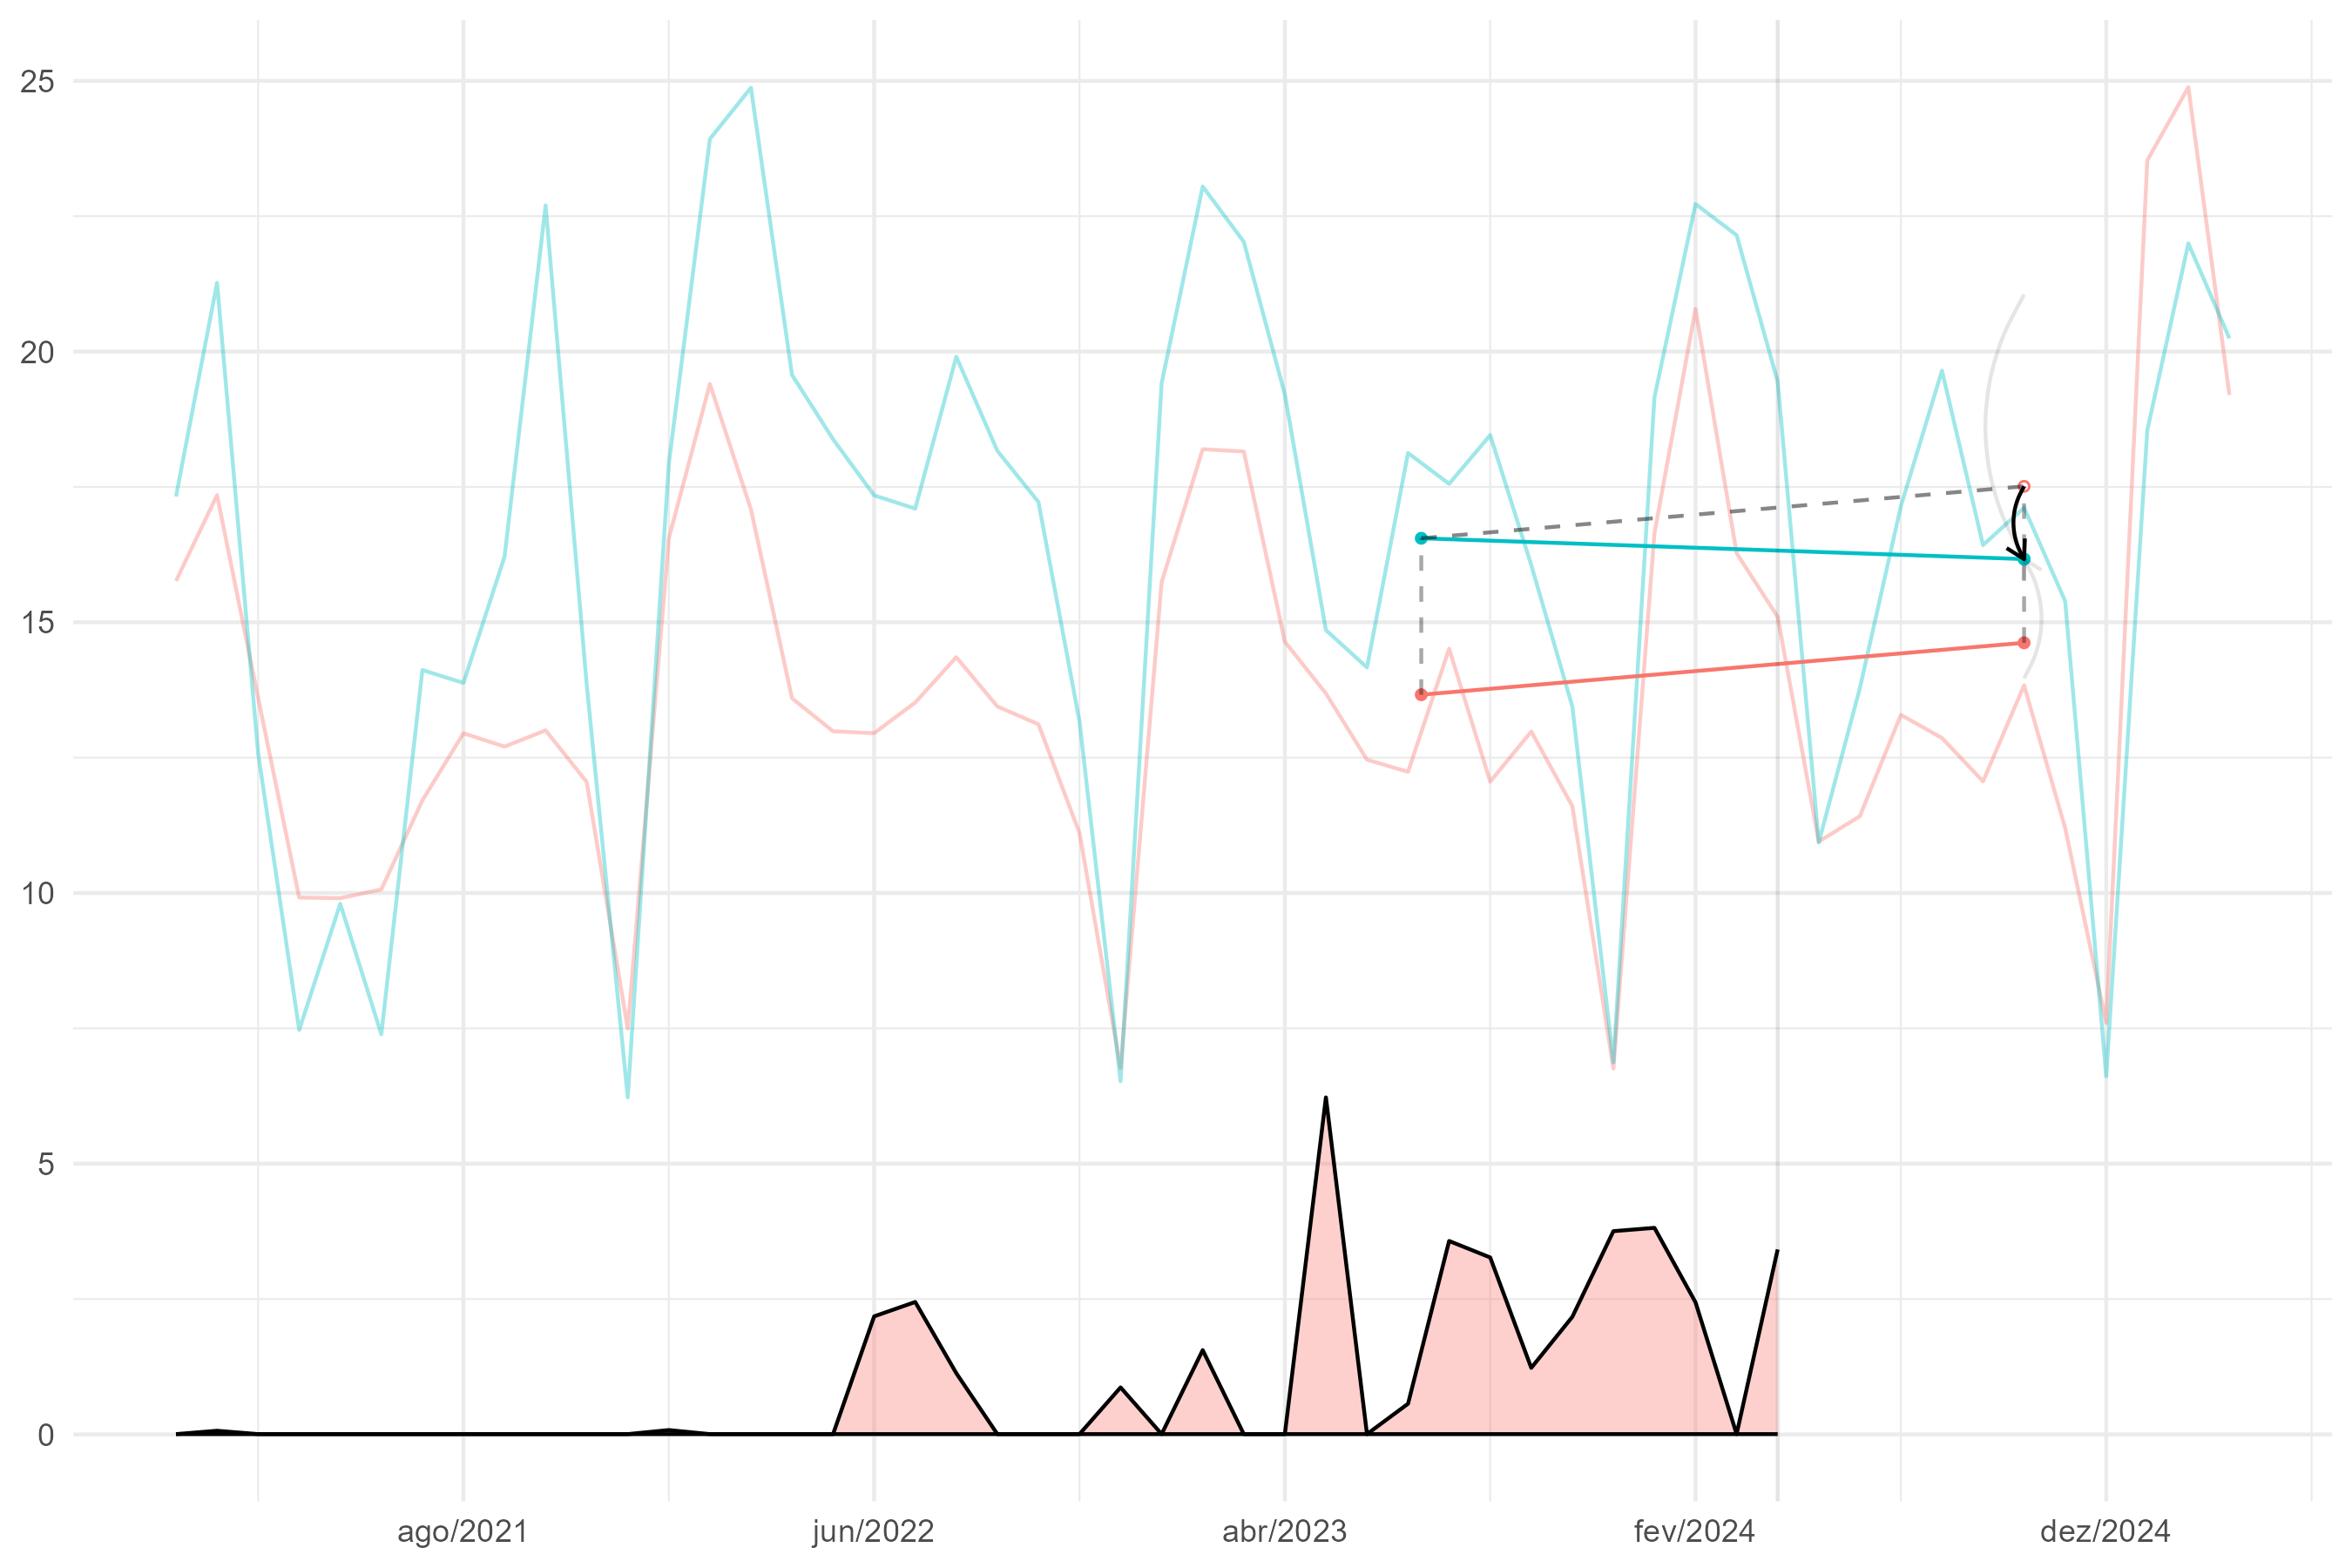
\includegraphics[width=0.47\textwidth]{municipio_4310108_completo_trajetorias.png}}
\caption{Trajetórias expandidas (3/3): municípios Arambaré e Igrejinha. Nenhum dos estimadores detecta efeito significante em ambos os casos. Pool completo, $N_0=193$. Fonte: elaboração própria.}
\label{fig:bex_par3}
\end{figure}

\end{document}